\documentclass[12pt,a4paper,twoside,openright]{report}
\let\openright=\cleardoublepage



%%% Choose a language %%%

\newif\ifEN
\ENtrue   % uncomment this for english
%\ENfalse   % uncomment this for czech

%%% Configuration of the title page %%%

\def\ThesisTitleStyle{mff} % MFF style
%\def\ThesisTitleStyle{cuni} % uncomment for old-style with cuni.cz logo
%\def\ThesisTitleStyle{natur} % uncomment for nature faculty logo

\def\UKFaculty{Faculty of Mathematics and Physics}
%\def\UKFaculty{Faculty of Science}

\def\UKName{Charles University in Prague} % this is not used in the "mff" style

% Thesis type names, as used in several places in the title
% \def\ThesisTypeTitle{\ifEN BACHELOR THESIS \else BAKALÁŘSKÁ PRÁCE \fi}
\def\ThesisTypeTitle{\ifEN MASTER THESIS \else DIPLOMOVÁ PRÁCE \fi}
%\def\ThesisTypeTitle{\ifEN RIGOROUS THESIS \else RIGORÓZNÍ PRÁCE \fi}
%\def\ThesisTypeTitle{\ifEN DOCTORAL THESIS \else DISERTAČNÍ PRÁCE \fi}
% \def\ThesisGenitive{\ifEN bachelor \else bakalářské \fi}
\def\ThesisGenitive{\ifEN master \else diplomové \fi}
%\def\ThesisGenitive{\ifEN rigorous \else rigorózní \fi}
%\def\ThesisGenitive{\ifEN doctoral \else disertační \fi}
% \def\ThesisAccusative{\ifEN bachelor \else bakalářskou \fi}
\def\ThesisAccusative{\ifEN master \else diplomovou \fi}
%\def\ThesisAccusative{\ifEN rigorous \else rigorózní \fi}
%\def\ThesisAccusative{\ifEN doctoral \else disertační \fi}



%%% Fill in your details %%%

% (Note: \xxx is a "ToDo label" which makes the unfilled visible. Remove it.)
\def\ThesisTitle{Improving Subword Tokenization Methods for Multilingual Models}
\def\ThesisAuthor{Jiří Balhar}
\def\YearSubmitted{2023}

% department assigned to the thesis
\def\Department{Institute of Formal and Applied Linguistics}
% Is it a department (katedra), or an institute (ústav)?
\def\DeptType{Institute}

\def\Supervisor{Ing. Tomasz Limisiewicz}
\def\SupervisorsDepartment{\xxx{Institute of Formal and Applied Linguistics}}

% Study programme and specialization
\def\StudyProgramme{Computer Science}
\def\StudyBranch{\xxx{IUI}}

\def\Dedication{%
Dedication. \xxx{It is nice to say thanks to supervisors, friends, family, book authors and food providers.}
}

\def\AbstractEN{%
\xxx{Abstracts are an abstract form of art. Use the most precise, shortest sentences that state what problem the thesis addresses, how it is approached, pinpoint the exact result achieved, and describe the applications and significance of the results. Highlight anything novel that was discovered or improved by the thesis. Maximum length is 200 words, but try to fit into 120. Abstracts are often used for deciding if a reviewer will be suitable for the thesis; a well-written abstract thus increases the probability of getting a reviewer who will like the thesis.}
% ABSTRACT IS NOT A COPY OF YOUR THESIS ASSIGNMENT!
}

\def\AbstractCS{%
\xxx{You will need to submit both Czech and English abstract to the SIS, no matter what language you use in the thesis. If writing in English, translate the contents of \texttt{\textbackslash{}AbstractEN} into this field. In case you do not speak czech, your supervisor should be able to help you with the translation.}
}

% 3 to 5 keywords (recommended), each enclosed in curly braces.
% Keywords are useful for indexing and searching for the theses by topic.
\def\Keywords{%
\xxx{{key} {words}}
}

% If your abstracts are long and do not fit in the infopage, you can make the
% fonts a bit smaller by this setting. (Also, you should try to compress your abstract more.)
% Alternatively, consider increasing the size of the page by uncommenting the
% geometry modification in thesis.tex.
\def\InfoPageFont{}
%\def\InfoPageFont{\small}  %uncomment to decrease font size

\ifEN\relax\else
% If you are writing a czech thesis, you additionally need to fill in the
% english translation of the metadata here!
\def\ThesisTitleEN{\xxx{Thesis title in English}}
\def\DepartmentEN{\xxx{Name of the department in English}}
\def\DeptTypeEN{\xxx{Department}}
\def\SupervisorsDepartmentEN{\xxx{Superdepartment}}
\def\StudyProgrammeEN{\xxx{study programme}}
\def\StudyBranchEN{\xxx{study branch}}
\def\KeywordsEN{%
\xxx{{key} {words}}
}
\fi


\usepackage[a-2u]{pdfx}

\ifEN\else\usepackage[czech,shorthands=off]{babel}\fi
\usepackage[utf8]{inputenc}
\usepackage[T1]{fontenc}

% See https://en.wikipedia.org/wiki/Canons_of_page_construction before
% modifying the size of printable area. LaTeX defaults are great.
% If you feel it would help anything, you can enlarge the printable area a bit:
%\usepackage[textwidth=390pt,textheight=630pt]{geometry}
% The official recommendation expands the area quite a bit (looks pretty harsh):
%\usepackage[textwidth=145mm,textheight=247mm]{geometry}

%%% FONTS %%%
\usepackage{lmodern} % TeX "original" (this sets up the latin mono)

% Optionally choose an override for the main font for typesetting:
\usepackage[mono=false]{libertinus} % popular for comp-sci (ACM uses this)
%\usepackage{tgschola} % Schoolbook-like (gives a bit of historic feel)
%\usepackage[scale=0.96]{tgpagella} % Palladio-like (popular in formal logic).
% IBM Plex font suite is nice but requires us to fine-tune the sizes, also note
% that it does not directly support small caps (\textsc) and requires lualatex:
%\usepackage[usefilenames,RM={Scale=0.88},SS={Scale=0.88},SScon={Scale=0.88},TT={Scale=0.88},DefaultFeatures={Ligatures=Common}]{plex-otf}

% Optionally choose a custom sans-serif fonts (e.g. for figures and tables).
% Default sans-serif font is usually Latin Modern Sans. Some font packages
% (e.g. libertinus) replace that with a better matching sans-serif font.
%\usepackage{tgheros} % recommended and very readable (Helvetica-like)
%\usepackage{FiraSans} % looks great
% DO NOT typeset the main text in sans-serif font!
% The serifs make the text easily readable on the paper.

% IMPORTANT FONT NOTE: Some fonts require additional PDF/A conversion using
% the pdfa.sh script. These currently include only 'tgpagella'; but various
% other fonts from the texlive distribution need that too (mainly the Droid
% font family).


% some useful packages
\usepackage{microtype}
\usepackage{amsmath,amsfonts,amsthm,bm}
\usepackage{graphicx}
\usepackage{xcolor}
\usepackage{booktabs}
\usepackage{caption}
\usepackage{floatrow}

% add my additional packages
\usepackage{mathtools}
\usepackage{bbm}

% load bibliography tools
\usepackage[backend=bibtex,natbib,style=numeric,sorting=none]{biblatex}
% alternative with alphanumeric citations (more informative than numbers):
%\usepackage[backend=bibtex,natbib,style=alphabetic]{biblatex}
%
% alternatives that conform to iso690
% (iso690 is not formally required on MFF, but may help elsewhere):
%\usepackage[backend=bibtex,natbib,style=iso-numeric,sorting=none]{biblatex}
%\usepackage[backend=bibtex,natbib,style=iso-alphabetic]{biblatex}
%
% additional option choices:
%  - add `giveninits=true` to typeset "E. A. Poe" instead of full Edgar Allan
%  - `terseinits=true` additionaly shortens it to nature-like "Poe EA"
%  - add `maxnames=10` to limit (or loosen) the maximum number of authors in
%    bibliography entry before shortening to `et al.` (useful when referring to
%    book collections that may have hundreds of authors)
%  - for additional flexibility (e.g. multiple reference sections, etc.),
%    remove `backend=bibtex` and compile with `biber` instead of `bibtex` (see
%    Makefile)
%  - `sorting=none` causes the bibliography list to be ordered by the order of
%    citation as they appear in the text, which is usually the desired behavior
%    with numeric citations. Additionally you can use a style like
%    `numeric-comp` that compresses the long lists of citations such as
%    [1,2,3,4,5,6,7,8] to simpler [1--8]. This is especially useful if you plan
%    to add tremendous amounts of citations, as usual in life sciences and
%    bioinformatics.
%  - if you don't like the "In:" appearing in the bibliography, use the
%    extended style (`ext-numeric` or `ext-alphabetic`), and add option
%    `articlein=false`.
%
% possibly reverse the names of the authors with the default styles:
%\DeclareNameAlias{default}{family-given}

% load the file with bibliography entries
\addbibresource{zotero}
% \addbibresource{refs}

% remove this if you won't use fancy verbatim environments
\usepackage{fancyvrb}

% remove this if you won't typeset TikZ graphics
\usepackage{tikz}
\usetikzlibrary{positioning} %add libraries as needed (shapes, decorations, ...)

% remove this if you won't typeset any pseudocode
\usepackage{algpseudocode}
\usepackage{algorithm}

% remove this if you won't list any source code
\usepackage{listings}


\hypersetup{unicode}
\hypersetup{breaklinks=true}

\usepackage[noabbrev]{cleveref}

\usepackage[normalem]{ulem}
\usepackage{caption}
\usepackage{subcaption}
% various forms of TODOs (you should remove this before submitting)
\usepackage[textsize=tiny, backgroundcolor=yellow!25, linecolor=black!25]{todonotes}
\newcommand{\xxx}[1]{\textcolor{red!}{#1}}
\definecolor{orange}{rgb}{1,0.5,0}
\newcommand{\tomasz}[1]{\textcolor{orange!}{TOMASZ: #1}}
\newcommand{\tomaszrep}[2]{\tomasz{\sout{#1} #2}} % remove this before compiling the final version


% use this for typesetting a chapter without a number, e.g. intro and outro
\def\chapwithtoc#1{\chapter*{#1}\addcontentsline{toc}{chapter}{#1}}

% If there is a line/figure overflowing into page margin, this will make the
% problem evident by drawing a thick black line at the overflowing spot. You
% should not disable this.
\overfullrule=3mm

% The maximum stretching of a space. Increasing this makes the text a bit more
% sloppy, but may prevent the overflows by moving words to next line.
\emergencystretch=1em

\ifEN
\theoremstyle{plain}
\newtheorem{thm}{Theorem}
\newtheorem{lemma}[thm]{Lemma}
\newtheorem{claim}[thm]{Claim}
\newtheorem{defn}{Definition}
\theoremstyle{remark}
\newtheorem*{cor}{Corollary}
\else
\theoremstyle{plain}
\newtheorem{thm}{Věta}
\newtheorem{lemma}{Lemma}
\newtheorem{claim}{Tvrzení}
\newtheorem{defn}{Definice}
\theoremstyle{remark}
\newtheorem*{cor}{Důsledek}
\fi

\newenvironment{myproof}{
  \par\medskip\noindent
  \textit{\ifEN Proof \else Důkaz \fi}.
}{
\newline
\rightline{$\qedsymbol$}
}

% real/natural numbers
\newcommand{\R}{\mathbb{R}}
\newcommand{\N}{\mathbb{N}}

% bold vectors instead of arrows
\let\vec\mathbf

% asymptotic complexity
\newcommand{\asy}[1]{\mathcal{O}(#1)}

% listings and default lstlisting config (remove if unused)
\DeclareNewFloatType{listing}{}
\floatsetup[listing]{style=ruled}

\DeclareCaptionStyle{thesis}{style=base,font={small,sf},labelfont=bf,labelsep=quad}
\captionsetup{style=thesis}
\captionsetup[algorithm]{style=thesis,singlelinecheck=off}
\captionsetup[listing]{style=thesis,singlelinecheck=off}

% Customization of algorithmic environment (comment style)
\renewcommand{\algorithmiccomment}[1]{\textcolor{black!25}{\dotfill\sffamily\itshape#1}}

% Uncomment for table captions on top. This is sometimes recommended by the
% style guide, and even required for some publication types.
%\floatsetup[table]{capposition=top}
%
% (Opinionated rant:) Captions on top are not "compatible" with the general
% guideline that the tables should be formatted to be quickly visually
% comprehensible and *beautiful* in general (like figures), and that the table
% "head" row (with column names) should alone communicate most of the content
% and interpretation of the table. If you just need to show a long boring list
% of numbers (because you have to), either put some effort into showing the
% data in an attractive figure-table, or move the data to an attachment and
% refer to it, so that the boredom does not impact the main text flow.
%
% You can make the top-captions look much less ugly by aligning the widths of
% the caption and the table, with setting `framefit=yes`, as shown below.  This
% additionally requires some extra markup in your {table} environments; see the
% comments in the example table in `ch2.tex` for details.
%\floatsetup[table]{capposition=top,framefit=yes}

\ifEN\floatname{listing}{Listing}
\else\floatname{listing}{Výpis kódu}\fi
\lstset{ % use this to define styling for any other language
  language=C++,
  tabsize=2,
  showstringspaces=false,
  basicstyle=\footnotesize\tt\color{black!75},
  identifierstyle=\bfseries\color{black},
  commentstyle=\color{green!50!black},
  stringstyle=\color{red!50!black},
  keywordstyle=\color{blue!75!black}}

% Czech versions of the used cleveref references (It's not as convenient as in
% English because of declension, cleveref is limited to sg/pl nominative. Use
% plain \ref to dodge that.)
\ifEN\relax\else
\crefname{chapter}{kapitola}{kapitoly}
\Crefname{chapter}{Kapitola}{Kapitoly}
\crefname{section}{sekce}{sekce}
\Crefname{section}{Sekce}{Sekce}
\crefname{subsection}{sekce}{sekce}
\Crefname{subsection}{Sekce}{Sekce}
\crefname{subsubsection}{sekce}{sekce}
\Crefname{subsubsection}{Sekce}{Sekce}
\crefname{figure}{obrázek}{obrázky}
\Crefname{figure}{Obrázek}{Obrázky}
\crefname{table}{tabulka}{tabulky}
\Crefname{table}{Tabulka}{Tabulky}
\crefname{listing}{výpis}{výpisy}
\Crefname{listing}{Výpis}{Výpisy}
\floatname{algorithm}{Algoritmus}
\crefname{algorithm}{algoritmus}{algoritmy}
\Crefname{algorithm}{Algoritmus}{Algoritmy}
\newcommand{\crefpairconjunction}{ a~}
\newcommand{\crefrangeconjunction}{ a~}
\fi

\renewcommand{\chapterautorefname}{Chapter} % use this file for various custom definitions


\begin{document}

% the layout is mandatory, edit only in dire circumstances

\pagestyle{empty}
\hypersetup{pageanchor=false}
\begin{center}

% top part of the layout, this actually differs between faculties

\def\ThesisTitleXmff{%
  \ifEN
    \centerline{\mbox{\includegraphics[width=166mm]{img/logo-en.pdf}}}
  \else
    \centerline{\mbox{\includegraphics[width=166mm]{img/logo-cs.pdf}}}
  \fi
  \vspace{-8mm}\vfill%
  {\bf\Large\ThesisTypeTitle}
  \vfill%
  {\LARGE\ThesisAuthor}\par
  \vspace{15mm}%
  {\LARGE\bfseries\ThesisTitle}
  \vfill%
  \Department}
\def\ThesisTitleCuniLogo#1{%
  {\large\UKName\par\medskip\par\UKFaculty }
  \vfill%
  {\bf\Large\ThesisTypeTitle}
  \vfill%
  \includegraphics[width=70mm]{#1}
  \vfill%
  {\LARGE\ThesisAuthor}\par
  \vspace{15mm}%
  {\LARGE\bfseries\ThesisTitle}
  \vfill%
  \Department\par}
\def\ThesisTitleXcuni{\ThesisTitleCuniLogo{img/uklogo.pdf}}
\def\ThesisTitleXnatur{\ThesisTitleCuniLogo{img/naturlogo.pdf}}

% choose the correct page and print it
\csname ThesisTitleX\ThesisTitleStyle\endcsname
% latex corner: X is the new @

\vfill

{
\centerline{\vbox{\halign{\hbox to 0.45\hsize{\hfil #}&\hskip 0.5em\parbox[t]{0.45\hsize}{\raggedright #}\cr
\ifEN Supervisor of the \ThesisGenitive thesis:
\else Vedoucí \ThesisGenitive práce: \fi
& \Supervisor \cr
\noalign{\vspace{2mm}}
\ifEN Study programme: \else Studijní program: \fi
& \StudyProgramme \cr
\noalign{\vspace{2mm}}
\ifEN Study branch: \else Studijní obor: \fi
& \StudyBranch \cr
}}}}

\vfill

\ifEN Prague \else Praha \fi
\YearSubmitted

\end{center}

\newpage

% remember to sign this!
\openright
\hypersetup{pageanchor=true}
\pagestyle{plain}
\pagenumbering{roman}
\vglue 0pt plus 1fill

\ifEN
\noindent
I declare that I carried out this \ThesisAccusative thesis independently, and only with the cited
sources, literature and other professional sources. It has not been used to obtain another
or the same degree.
\else
\noindent
Prohlašuji, že jsem tuto \ThesisAccusative práci vypracoval(a) samostatně a výhradně
s~použitím citovaných pramenů, literatury a dalších odborných zdrojů.
Tato práce nebyla využita k získání jiného nebo stejného titulu.
\fi

\ifEN
\medskip\noindent
I understand that my work relates to the rights and obligations under the Act No.~121/2000 Sb.,
the Copyright Act, as amended, in particular the fact that the Charles
University has the right to conclude a license agreement on the use of this
work as a school work pursuant to Section 60 subsection 1 of the Copyright~Act.
\else
\medskip\noindent
Beru na~vědomí, že se na moji práci vztahují práva a povinnosti vyplývající
ze zákona č. 121/2000 Sb., autorského zákona v~platném znění, zejména skutečnost,
že Univerzita Karlova má právo na~uzavření licenční smlouvy o~užití této
práce jako školního díla podle §60 odst. 1 autorského zákona.
\fi

\vspace{10mm}


\ifEN
\hbox{\hbox to 0.5\hsize{%
In \hbox to 6em{\dotfill} date \hbox to 6em{\dotfill}
\hss}\hbox to 0.5\hsize{\dotfill\quad}}
\smallskip
\hbox{\hbox to 0.5\hsize{}\hbox to 0.5\hsize{\hfil Author's signature\hfil}}
\else
\hbox{\hbox to 0.5\hsize{%
V \hbox to 6em{\dotfill} dne \hbox to 6em{\dotfill}
\hss}\hbox to 0.5\hsize{\dotfill\quad}}
\smallskip
\hbox{\hbox to 0.5\hsize{}\hbox to 0.5\hsize{\hfil Podpis autora\hfil}}
\fi

\vspace{20mm}
\newpage

% dedication

\openright

\noindent
\Dedication

\newpage

% mandatory information page

\openright

\vbox to 0.49\vsize{\InfoPageFont
\setlength\parindent{0mm}
\setlength\parskip{5mm}

\ifEN Title: \else Název práce: \fi
\ThesisTitle

\ifEN Author: \else Autor: \fi
\ThesisAuthor

\DeptType:
\Department

\ifEN Supervisor: \else Vedoucí \ThesisGenitive práce: \fi
\Supervisor, \SupervisorsDepartment

\ifEN Abstract: \AbstractEN \else Abstrakt: \AbstractCS \fi

\ifEN Keywords: \else Klíčová slova: \fi
\Keywords

\vss}\ifEN\relax\else\nobreak\vbox to 0.49\vsize{\InfoPageFont
\setlength\parindent{0mm}
\setlength\parskip{5mm}

Title:
\ThesisTitleEN

Author:
\ThesisAuthor

\DeptTypeEN:
\DepartmentEN

Supervisor:
\Supervisor, \SupervisorsDepartmentEN

Abstract:
\AbstractEN

Keywords:
\KeywordsEN

\vss}
\fi

\newpage

\openright
\pagestyle{plain}
\pagenumbering{arabic}
\setcounter{page}{1}


\tableofcontents


\chapter{Introduction}

% Introduction should answer the following questions, ideally in this order:
% \begin{enumerate}
% \item What is the nature of the problem the thesis is addressing?
% \item What is the common approach for solving that problem now?
% \item How this thesis approaches the problem?
% \item What are the results? Did something improve?
% \item What can the reader expect in the individual chapters of the thesis?
% \end{enumerate}

% Expected length of the introduction is between 1--4 pages. Longer introductions may require sub-sectioning with appropriate headings --- use \texttt{\textbackslash{}section*} to avoid numbering (with section names like `Motivation' and `Related work'), but try to avoid lengthy discussion of anything specific. Any ``real science'' (definitions, theorems, methods, data) should go into other chapters.
% \todo{You may notice that this paragraph briefly shows different ``types'' of `quotes' in TeX, and the usage difference between a hyphen (-), en-dash (--) and em-dash (---).}


\xxx{Image: text in three languages, tokenized text in three languages, multilingual model, classification head, outputs for each example}

\tomasz{It's my comment.}
% large multilingual models
Large neural language models have been shown to perform well on a variety of Natural Language Processing (NLP) tasks and have become a de-facto standard for tackling tasks that require language understanding. The main advantage of these pretrained models is that they are able to leverage a large, unannotated pretraining corpus. After pretraining, we usually need only a fraction of annotated, task-specific data for finetuning the model for the task at hand. \cite{devlin_bert_2019,radford_improving_nodate} \tomasz{I don't like the last sentence -> ... to perform well in other/less resourcefull languages.} Multilingual pretrained models extend the pretrain-finetune paradigm to multiple languages. By pretraining on large, \textit{multilingual} corpus, these models provide high quality representations even for low-resource languages where a dedicated monolingual model might not even exist. Furthermore, it has been shown that finetuning a multilingual model with data from a high-resource language makes the model capable to perform the task at hand in the other languages it has been pre-trained on. This "cross-lingual transfer", a phenomenon specific to multilingual models, allows the usage of the model for languages where task-specific data is not available. \cite{k_cross-lingual_2022,conneau_unsupervised_2020-1}

Even though multilingual models are capable of narrowing the gap between high-resource languages and low-resource languages, they still suffer from the fact that the languages are not equally represented in the pretraining data. This leads to a lower performance on the low-resource languages. \cite{conneau_unsupervised_2020} Furthermore, \Citeauthor{conneau_unsupervised_2020} has shown that increasing the number of languages while keeping the model size fixed leads to a decrease in performance across all languages, tradeoff referred to as the \textit{curse of multilinguality}. \cite{conneau_unsupervised_2020} \tomasz{I don't like this term (CoM), IMO it's overused and vague.}

% what is tokenization
Tokenization is the crucial first step we take when tackling a NLP problem. In simple terms, tokenization converts an input text into a sequence of tokens. The tokens are then used as the input for the NLP methods. Traditionally, the term tokenization referred to the methods of splitting up an input text into words as a preprocessing step for NLP methods. \tomaszrep{After}{With} the advent of large neural models, we have seen a shift towards using subword tokenization methods such as Byte Pair Encoding (BPE) \cite{sennrich_neural_2016}, Unigram Language Model \cite{kudo_sentencepiece_2018} or Wordpiece \cite{devlin_bert_2019}. \tomasz{Use logical connector here, subword tokenizers used because ...}These methods split up words into subword units and therefore one word might become encoded as a series of short subwords. These subword tokens are then used as the input tokens for the neural models. \xxx{maybe do not specify the tokenization methods here. Dedicate the space to connecting the tokenization with the multilingual models.} \tomasz{I agree with the first suggestion..}

It has been shown that the choice of tokenization method has a significant effect on the performance of the NLP models - whether we talk about monolingual language models \cite{bostrom_byte_2020}, multilingual models \cite{rust_how_2021} or machine translation models \cite{kudo_sentencepiece_2018,gowda_finding_2020}. In the context of multilingual language models, the tokenization methods \tomaszrep{need to be able}{} to handle more than a hundred languages at once. This is a challenging task, as the languages differ in their morphology, orthography and \tomaszrep{other properties}{script}. Another challenge is, as mentioned before, the fact that the languages are not equally represented in the training data. \Citeauthor{rust_how_2021} have shown that the low-resource languages are under-represented in the tokenizer vocabularies. This leads to performance loss, that can be mitigated by changing the vocabulary to one with more language-specific tokens. \cite{rust_how_2021}

\xxx{in the thesis annotation, we say that we look for an optimal tokenization method for multilingual language models. This of course depends on how we define optimal. I think I should connect the focus on low-resource languages with the definition of optimal.}

\xxx{rewrite the introduction so that the research question are a natural consequence of the introduction - the reader should be able to guess the research questions from the introduction}

In this thesis we study the effect of tokenization on the performance of multilingual pretrained models. \xxx{why; We propose metrics to be able to assess the differences between tokenizers before costly pretrainig. We can use these metrics to compare between methods, see the differences in what they do and choosing the best option for our usecase} First we examine what properties of the tokenizers are desirable for multilingual models with respect to low- and high- resource languages. To this end, we propose three metrics --- Characters per Token, Average Rank and Jensen-Shannon Divergence between token distributions --- for measuring the quality of tokenization across the target languages. First two metrics aim to measure how well is each language represented in the multilingual vocabulary. We coin this property as \textit{vocabulary allocation}. The third metric measures the \textit{vocabulary overlap} --- to what degree are the tokens shared between languages. We show that these metrics correlate with the representation quality of the model on the downstream tasks.\xxx{why is the correlation needed?} \xxx{maybe motivate more why we need these metrics}

% we propose simple baselines for balancing the vocabulary that perform on par with more complex methods
Then we examine and reproduce three tokenization methods \citep{chung_improving_2020,zheng_allocating_2021,liang_xlm-v_2023} proposed to tackle the problem of suboptimal tokenization and underrepresentation of low-resource languages in multilingual models. \xxx{before this sentence: why do we need the balancing methods} In our scaled-down setting, we compare these methods with two simpler baseline methods we propose. The first baseline method \xxx{name} is simply to sample the languages uniformly during the tokenizer training. The second method \xxx{name} takes the balancing one step further and resamples the word distributions in hopes of leveling a hypothesized topic imbalance across the languages. 
Gathering all five tokenization methods together, we then measure their \textit{vocabulary allocation} and \textit{vocabulary overlap} using the metrics we proposed and validated before. We select the best tokenization method and compare it with our baseline methods on downstream tasks. We show that in our setting, the baseline methods perform on par with the more complex methods proposed in the literature. \xxx{we posit that the tokenization is a zero-sum game and by clustering or training separate tokenizers for each language, we only shift the performance from one language to another.}
\tomasz{I don't think you can say that. If you have a bad toknizer all the languages are affected.}

% - We show that all balancing methods improve the performance of the model on the word-level downstream tasks

\section{Contributions}

The work on this thesis began as a collaboration with Ing. Tomasz Limisiewicz on the paper \Citetitle{limisiewicz_tokenization_2023}. The paper was accepted to the \textit{ACL Findings 2023} and will be published in July 2023. The contributions of this paper, included in this thesis are as follows:

\begin{itemize}
    \item Proposal of metrics for measuring the quality of tokenization for multilingual models.
    \item Validation of the metrics on a multitude of downstream tasks using four different tokenization methods.
\end{itemize}

Additionally, the thesis continues in the multilingual tokenization research by:

\begin{itemize}
    \item Investigating the effect of important choices in the tokenization process on the quality of the tokenization.
    \item Reproducing three tokenization methods proposed in the literature.
    \item Proposing two simpler, alternative methods for improving the tokenization for low-resource languages.
    \item Comparing the tokenization methods on downstream tasks and showing that the simpler methods perform on par with the more complex methods.
\end{itemize}

\section{Research Questions}


- (Q1) How do sub-word tokenizers differ in overlap and allocation of learned vocabularies?
- (Q2) Which properties of multilingual tokenizers affect the LM’s representation quality?

\xxx{TODO}


% summary of the thesis structure with links to the chapters
The thesis is structured as follows: In Chapter 1 we provide the necessary background on tokenization and multilingual models.  \xxx{TODO}

% from methodology:

% The main goal of the thesis is to \textbf{improve multilingual models with better tokenization}. The standard procedure followed by most of the large multilingual models is to train the tokenizer on the joint, multilingual corpus used for training the model \cite{mielke_between_2021,conneau_unsupervised_2020,conneau_cross-lingual_nodate}. As many authors pointed out \cite{wang_improving_2019,chung_improving_2020,rust_how_2021}, by using this simple approach the resulting tokenizer overtokenizes some of the low-resource languages, especially those that do not use the latin script. The latin script tokens appear more often in the resulting vocabulary because the procedure of merging all corpora together greatly increases the occurence statistics of the Latin character n-grams. \cite{zheng_allocating_2021}

% To this end, several methods of mitigating this issue were suggested. \citet{chung_improving_2020} proposed a method based on creating multiple clusters of corpora instead of one joint cluster. The multilingual tokenizer is then created by merging together smaller, specialized tokenizers trained on these clusters. \citet{zheng_allocating_2021} proposed a method of allocating the vocabulary budget to the languages based on a heuristic function similar to entropy. \citet{liang_xlm-v_2023} showed that by combining the two approaches, the resulting tokenizer scales better to larger vocabulary sizes.

% Unrelated to multilingual models, we have seen also other approaches of tokenizer improvement related to Domain Adaptation. In the paper \Citetitle{gururangan_dont_2020}, \citeauthor{gururangan_dont_2020} \cite{gururangan_dont_2020} showed that a continued pretraining models on a domain-specific data leads to performance improvements of in-domain tasks. \citet{sachidananda_efficient_2021} showed that these improvements can be achieved not only by costly pretraining continuation but also by simply extending the model vocabulary with a small amount of domain-specific tokens that are then fine-tuned on the domain tasks.

% \xxx{rewrite this paragraph}
% In this thesis we first replicate the results of \citet{chung_improving_2020}, \citet{zheng_allocating_2021} and \citet{liang_xlm-v_2023} on our selected subset of languages. We then use our evaluation framework of \citet{limisiewicz_tokenization_2023} to compare these methods and pick a strong baseline. We then present our novel method of improving the tokenizer based on a extension of the clustering idea of \citet{chung_improving_2020}.


% Example pseudo-code from the original thesis template:
% \begin{algorithm}
%     \begin{algorithmic}
%     \Function{ExecuteWithHighProbability}{$A$}
%         \State $r \gets$ a random number between $0$ and $1$
%         \State $\varepsilon \gets 0.0000000000000000000000000000000000000042$
%         \If{$r\geq\varepsilon$}
%             \State execute $A$ \Comment{We discard the return value}
%         \Else
%             \State print: \texttt{Not today, sorry.}
%         \EndIf
%     \EndFunction
%     \end{algorithmic}
%     \caption{Algorithm that executes an action with high probability. Do not care about formal semantics in the pseudocode --- semicolons, types, correct function call parameters and similar nonsense from `realistic' languages can be safely omitted. Instead make sure that the intuition behind (and perhaps some hints about its correctness or various corner cases) can be seen as easily as possible.}
%     \label{alg:w}
% \end{algorithm}



\chapter{Background}
\label{chap:background}

% \xxx{In this chapter we discuss the related work in the field of subword tokenization and multilingual pretrained models. We start with a brief overview of the subword tokenization methods and then discuss the multilingual pretrained models. We also discuss the work that has been done in the field of multilingual subword tokenization.}

% In order to organize Chapter Two, you will first start with an introduction about the general problem and your topic. Then you will provide an advance organizer, which indicates what will be covered in the literature review.

In this thesis, we investigate the effect of subword tokenization on the performance of multilingual pretrained models. To that end, we first introduce multilingual language models. Then, we explain the concept of subword tokenization and the most common subword tokenization methods. Lastly, we show what problems arise when using pretrained models in multilingual settings and what methods have been proposed to mitigate these problems.

\tomasz{Rewrite the intro: Be more clear and sepecific}
\tomasz{Genearal remark: you may create separate section summarizing the metrics of allocation (e.g. fertility, ALP) ala overlap (e.g. Wasserstein)}

\section{Multilingual language models}

In recent years we have seen a dramatic rise in the use of neural language models. The premise of these models is the ability to learn unsupervised from large amounts of unlabeled data. 

We focus on studying the properties of \textbf{multilingual} language models following \citet{devlin_bert_2019} (mBERT)\footnote{We cite the monolingual BERT paper as the mBERT model does not have an associated publication. In the literature, sometimes the mBERT Github README is cited for the multilingual variant\cite{devlin_bertmultilingualmd_2019}} and \citet{conneau_unsupervised_2020} (XLM-R). In these works, a Transformer \cite{vaswani_attention_nodate} based multilingual masked language model is pretrained on sentences sampled from a multilingual corpus of around 100 languages. This allows for cross-lingual transfer, which the authors show on a variety of language understanding tasks.

The multilingual models such as mBERT or XLM-R are composed of the tokenizer, which splits the input text into tokens, the embedding matrix, which encodes the tokens into a sequence of word embeddings, and the Transformer encoder, which transforms the sequence of word embeddings into a sequence of so-called contextualized embeddings. The contextualized embeddings are then fed into a task-specific output layer --- usually a linear layer with a softmax activation. The pretraining is done using the masked language modeling task, where some of the input tokens are stochastically masked out and the model is trained to predict the masked tokens \cite{devlin_bert_2019}.

In the case of XLM-R \cite{conneau_unsupervised_2020}, the pretraining is performed on data from 100 languages. The tokenization uses a joint vocabulary for all languages and the model is trained to predict the masked tokens in all languages at once. Even without any supervision, the model is shown to perform well on a variety of cross-lingual tasks.

The tasks that are usually used to evaluate the performance of the pretrained models are the following \cite{ruder_xtreme-r_2021}:

\begin{itemize}
    
    \item \textbf{Question Answering (QA):} This task involves predicting an answer to a question given a context. The context usually consists of a paragraph of text and the model must locate and return the correct answer from this text.
    \item \textbf{Natural Language Inference (NLI):} In this task, the model is given a pair of sentences and it has to determine the relationship between them: whether they contradict each other, they are logically consistent, or they are unrelated.
    \item \textbf{Part-of-Speech Tagging (POS):} This is a classic task in NLP where each word in a sentence is assigned a tag that represents its syntactic role (e.g., noun, verb, adjective, etc.).
    \item \textbf{Named Entity Recognition (NER):} NER involves identifying and classifying named entities in text into predefined categories such as person names, organizations or locations.
    \item \textbf{Cross-lingual Sentence Retrieval:} In this task, the model is given a query sentence in one language and a collection of candidate sentences in a different language. The goal is to retrieve the sentences from the candidate pool that are the translation of the query.
\end{itemize}
    
These tasks cover a broad spectrum of capabilities, testing basic linguistic understanding and complex reasoning skills. The performance of the pretrained model on these tasks provides a comprehensive measure of its cross-lingual abilities.


% In this thesis, we are interested in the effect of tokenization on the pretrained models. The tokenization step is the first step in the preprocessing pipeline of the pretrained models. It is the step where the input text is split into tokens, which are then used as the input to the neural model. The tokenization step is important because it can affect the performance of the model. For example, if the tokenization method splits a word into two tokens, the model will not be able to learn the meaning of the word as a whole.

% At the inference step, the masked language models work by first tokenizing the input sentence, embedding each token as a vector using the learned embedding matrix, passing the embeddings through a Transformer encoder and then 

% terms I use later that need explaination:
% - embedding layer of mBERT, embedding matrix
% - model size
% - masked language models
% - freezing a model

% QA, NER, NLI, POS
% paraphrase identification


% \xxx{TODO}

% Language modeling is a task where we predict the next word given the previous words. \cite{manning_foundations_1999} More formally, given a sequence of words $w_1, w_2, \dots, w_{m-1}$, the language model computes the probability of the next word $w_{m}$:

% \begin{equation}
%     P(w_{m} | w_1, w_2, \dots, w_{m-1})
% \end{equation}

% One method to compute this probability is to use n-gram language models. These models simplify the problem by making a Markov assumption --- the probability of the next word is conditioned only on the previous $n-1$ words:

% \begin{equation}
%     P(w_{m} | w_1, w_2, \dots, w_{m-1}) \approx P(w_{m} | w_{m-n+1}, w_{m-n+2}, \dots, w_{m-1})
% \end{equation}

% \xxx{TODO}

% \section{Multilingual pretrained models}

% \xxx{TODO}

% \subsection{Assessing the ability of multilingual models}

% - word level tasks
% - sentence level tasks
% - inlanguage vs crosslingual

\section{Subword tokenization}

Subword tokenization methods split up words into subword units, which are then used as the input tokens for the neural models. This step is generally needed for pretrained models because including all words in the model vocabulary would be computationally infeasible. Subword tokenization allows scaling down the vocabulary size by splitting up rare words into subword units. Another advantage of subword tokenization over word tokenization is that it allows the model to generalize to unseen words by composing the embeddings of the subword units. For word tokenization methods, the missing words are called out-of-vocabulary tokens and subword tokenization methods mitigate largely this issue. In this section, we describe the most common subword tokenization methods used in large multilingual language models.

% This is done to mitigate the out-of-vocabulary (OOV) problem and to reduce the computational complexity of the softmax cross-entropy loss over a very large output vocabulary. The most common subword tokenization methods are Byte Pair Encoding (BPE), Unigram LM and Wordpiece.

% \xxx{TODO: define vocabulary - set of all tokens, vocabulary size}

\subsection{Byte Pair Encoding (BPE)}

The Byte Pair Encoding (BPE) algorithm was introduced by \citet{sennrich_neural_2016}. They have adapted a compression algorithm \cite{gage_new_1994} to learn a subword vocabulary from a corpus. This method was shown to improve the performance of neural machine translation (NMT) models. BPE was subsequently used for some of the well-known pretrained models such as GPT-2 \citep{radford_improving_2018}.

The principle of BPE is to iteratively merge the most frequent byte pairs in the corpus until the vocabulary size reaches the target size. The algorithm starts with a vocabulary of unique characters used in the input corpus. Using this vocabulary, we then compute the frequency of every character pair and merge the most frequent pair to create a new subword unit. We recompute the frequency of the subword unit pairs and repeat the process until the target vocabulary size is reached.

To tokenize an input text, the BPE algorithm then iteratively merges the pairs in the same order as they were merged during training. The algorithm stops when it has merged all pairs in the vocabulary. The output of the algorithm is a sequence of subword units that can be used as the input tokens for the neural model.

\begin{algorithm}
    \begin{algorithmic}
        \Function{BPE}{$C$}
        \State $V \gets$ unique characters in $C$
        \While{$|V| < V_{target}$}
        \State $p \gets$ most frequent pair in $V$
        % \State $V \gets V \setminus p$
        \State $V \gets V \cup \{p\}$
        \EndWhile
        \State \Return $V$
        \EndFunction
    \end{algorithmic}
    \caption{The Byte Pair Encoding algorithm.}
    \label{alg:bpe}
\end{algorithm}

% \subsection{Byte-level BPE}


\subsection{Wordpiece}

First introduced in \cite{schuster_japanese_2012} the Wordpiece algorithm is a similar technique to BPE. It is used in the BERT \citep{devlin_bert_2019} masked language model. The training is based on a greedy merging of the subword units similar to BPE. Unlike BPE, Wordpiece does not use the frequency of the subword units to merge them. Instead, it merges the pair that maximizes the likelihood of an unigram language model trained on the corpus.

Contrary to BPE and Unigram LM, there is no official, public implementation of the original Wordpiece algorithm. There are several implementations of the algorithm available but these diverge from the original algorithm. For example, the implementation in the Huggingface library \citep{wolf_transformers_2020} does not use the unigram language model to merge the subword units. Instead, the training follows the BPE procedure and only adds prefixes to the subword units to mimic the output format of the BERT Wordpiece implementation. \footnote{See the \href{https://github.com/huggingface/tokenizers/blob/291b2e23ae81cf94738835852213ce120152d121/tokenizers/src/models/wordpiece/trainer.rs}{Wordpiece implementation} in the Huggingface Tokenizers library.}

% https://github.com/huggingface/tokenizers/blob/291b2e23ae81cf94738835852213ce120152d121/tokenizers/src/models/wordpiece/trainer.rs#L92

The implementation in the Tensorflow library follows a different, top-down approach to creating the subword vocabulary. It starts with a vocabulary of words and then iteratively splits the words into subword units to reach a target vocabulary size. \footnote{See the Tensorflow documentation for the \href{https://www.tensorflow.org/text/api_docs/python/text/WordpieceTokenizer}{Wordpiece tokenizer}.}

% 

\subsection{Unigram LM}
\label{sec:unigram}

The Unigram LM tokenizer, sometimes referred to as the SentencePiece tokenizer \citep{kudo_sentencepiece_2018}, was introduced by \citet{kudo_subword_2018}. The motivation for this method was to create a probabilistic model for subword tokenization. With this model, it is then possible to sample different segmentations of the input text. Training on these varied segmentations empirically improves the performance of the NMT models. In large language models such as XLM-R, the Unigram tokenizer is used deterministically, always choosing the most probable segmentation.

Given an input sentence $X$, the Unigram LM algorithm finds the most probable segmentation $x^\star$ for the input sentence X:

\begin{equation}
    x^\star = {\arg\max}_{x \in \mathcal{S}(X)} P(x)
\end{equation}


Where $\mathcal{S}(X)$ is the set of all possible segmentations of the input sentence $X$ given a subword vocabulary $\mathcal{V}$. The probability $P(x)$ of a segmentation $x$ is computed as a product of subword occurrence probabilities $p(x_i)$:

\begin{equation}
    P(x) = \prod_{i=1}^{|x|} p(x_i)
\end{equation}

Here, the subword occurrence probabilities cannot be computed using occurrence statistics in the corpus since we do not have the final vocabulary yet. Also, with a given vocabulary, there are usually many possibilities on how to segment the input sentence from character level granularity to word level. Instead, the Unigram LM uses the Expectation-Maximization (EM) algorithm to estimate the marginal subword occurrence probabilities $p(x_i)$ over all segmentation variants. The EM algorithm maximizes the marginal likelihood $\mathcal{L}$ with respect to the latent subword probabilities $p(x_i)$:

\begin{equation}
    \mathcal{L} = \sum_{s=1}^{|D|} \log (P(X^{(s)})) = \sum_{s=1}^{|D|} \log( \sum_{x \in \mathcal{S}(X^{(s)})} P(x) )
\end{equation}

By maximizing the marginal likelihood, the Unigram LM considers all possible segmentations of the input sentences when estimating the subword occurrence probabilities $p(x_i)$. After optimization of $p(x)$, it is then possible to compute the most probable segmentation $x^\star$ for a given input sentence $X$ using the Viterbi algorithm.

The training of the Unigram LM works in a top-down fashion. It starts with a large seed vocabulary of the most frequent character n-grams. The default setting is seeding the vocabulary with top 1M most frequent character n-grams with $n \leq 16$. These character n-grams are then iteratively pruned down to the target vocabulary size in the following way:

\begin{enumerate}
    \item With a given vocabulary $\mathcal{V}$, estimate the subword occurrence probabilities $p(x_i)$ using the EM algorithm.
    \item Segment the training corpus, sample the best segmentation for every sentence.
    \item For each subword $x_i$ in the vocabulary, compute the loss. The loss is defined as the decrease in the unigram language model likelihood if the subword is removed from the vocabulary.
    \item Keep the top 80\% of the subwords with the lowest loss.
    \item Repeat this process with the new vocabulary $\mathcal{V}$ until the target vocabulary size is reached.
\end{enumerate}

After the training, the Unigram LM algorithm outputs a subword vocabulary $\mathcal{V}$ and the corresponding marginal subword probabilities $p(x_i)$. Tokenization of a new input is then done by running the Viterbi algorithm to sample top-n segmentations of the input sentence. 

% \xxx{-> bostrom has really nice pseudocode}

% For a given vocabulary $\mathcal{V}$,

% The pruning is done using a unigram language model. With a subword vocabulary and corresponding subword occurence probabilities $p(x_i)$, the unigram language model computes the probability of a sentence $X$ as follows:

% The Unigram LM algorithm uses, as the name suggests, a unigram language model to learn the subword vocabulary. 


% With the default hyperparameter settings, the algorithm starts with an initial vocabulary of $1 000 000$ \todo{fix num} most frequent character ngrams found within the word boundaries. These character n-grams are then iteratively pruned down to the target vocabulary size. T

% The overview of the algorithm is as follows:

% 1. Create a large seed vocabulary

% 2. Repeat until the target vocabulary size is reached:


% (a). Optimize the subword occurence probabilities $p(x_i)$ using the EM algorithm (default value is 2 EM subiterations). The EM algorithm maximizes the marginal likelihood $\mathcal{L}$ with $p(x_i)$ as the latent variables:

% Expectation step: Compute the marginal probability of each subword $x_i$ using the current probabilities $p(x_i)$.

% Maximization step: Compute the new probabilities $p(x_i)$ using the expected number of occurrences $E(x_i)$.

% (b). Merge the n-gram with the highest probability

% Under the assumptions of the unigram language model, the probability of a sequence $x = ( x_1, \dots, x_n )$ is given by the product of the probabilities of the individual tokens $x_i$:

% \begin{equation}
%     P(x) = \prod_{i=1}^{n} P(x_i)
% \end{equation}

% The initial probability of the character n-grams is given by their frequency in the corpus over the sum of all frequencies:

% \begin{equation}
%     P(x_i) = \frac{f(x_i)}{\sum_{j=1}^{N} f(x_j)}
% \end{equation}

% \subsection{Alternative tokenization approaches (low priority)}

% \subsubsection{Character-level models}
% \subsubsection{Morphology based models}

% \section{Subword regularization (low priority)}

% \begin{enumerate}
%     \item bpe dropout
%     \item unigram lm
% \end{enumerate}


% \chapter{Related work}
% \label{chap:related_work}

\section{Tokenization with many languages}

Despite the recent advances in language modeling, the tokenization methods used in multilingual language models remain mostly unchanged. The first models trained on multiple languages, such as mBERT \cite{devlin_bert_2019,devlin_bertmultilingualmd_2019} and XLM \cite{lample_cross-lingual_2019} use the same tokenization methods as their monolingual versions - namely the Wordpiece and BPE algorithms. Later language models such as XLM-R \cite{conneau_unsupervised_2020}, mBART \cite{liu_multilingual_2020} or mT5 \cite{xue_mt5_2021} use the Unigram LM algorithm to learn the subword vocabulary. The most recent multilingual generative models, such as the 176B parameter BLOOM model \cite{scao_bloom_2022} or the XGLM \cite{lin_few-shot_2022} use the Byte-level BPE and Unigram LM algorithms respectively.

The methods these models use to tokenize the input text are the same as the ones used in the monolingual models. The main difference is that the tokenization training algorithm is run on all of pretraining data. This means that the tokenizer is trained on all languages at once. 

As we have pointed out previously, the pretraining data is not evenly distributed across languages. High-resource languages such as English or Indonesian may have hundreds of times the amount of training data than low-resource languages such as Swahili or Amharic.\footnote{By high-resource and low-resource languages, we mean languages with generally a lot or little data available in the pretraining corpora such as Wikipedia dumps or internet crawls. This may not necessarily correspond to the number of speakers of the language.}
% \tomasz{Here or even better before, explain what low-/high-resource mean, I.e. the distinction is made based on data available from the web not number of speakers. You may cite Joshi et al.}
% \tomasz{The following desciption should be in a separate section: Subsampling}


To account for the discrepancy in the number of training examples per language, the training data is usually subsampled with a bias towards low-resource languages. This subsampling is performed both for the model pretraining and the tokenizer training \cite{devlin_bertmultilingualmd_2019,lample_cross-lingual_2019}.

We describe the subsampling method in detail in \autoref{sec:data_sampling}. In a nutshell, the subsampling is done by adjusting the probability $p(l)$ of sampling a line from a language $l$. The probabilities are exponentiated with a factor $\alpha$ and renormalized to sum to 1. With $\alpha=0.0$, the subsampling is uniform across languages. With $\alpha=1.0$, the smoothing has no effect. The usual values chosen for this factor $\alpha$ are 0.7 \cite{devlin_bert_2019}. 0.5 \cite{lample_cross-lingual_2019} and 0.3 \cite{conneau_unsupervised_2020}. Throughout this thesis, we will refer to this subsampling method and the factor $\alpha$ often. When we refer to the factor $\alpha$, we mean the factor used for the tokenizer training. We will use a fixed, separate $\alpha$ for pretraining data sampling.

\subsection{Bias towards high-resource languages}

As \citet{rust_how_2021} have shown, the bias towards high-resource languages however still persists, even after subsampling the training data. The authors compare the performance of the multilingual model mBERT and language-specific variants of BERT. By finetuning and evaluating on five different tasks across nine typologically different languages, they show that there is a performance gap between the multilingual and monolingual models. By further examination they determine that the performance gap may be explained by 1) pretraining data size and 2) the choice of tokenizer and its suitability for the tested language. 

They show that the performance of mBERT can be improved for a specific language by switching to a monolingual vocabulary and retraining only the embedding layer of mBERT. The model with a dedicated vocabulary outperforms the vanilla mBERT on a variety of tasks, which indicates that the multilingual vocabulary of mBERT is not optimal. 

But what changes when we switch to a monolingual vocabulary and why does it improve the multilingual model to the point it approaches the performance of the dedicated monolingual model? \citet{rust_how_2021} propose to look at how often the tokenizer segments words. They show that for some languages, the multilingual tokenizer splits words into subwords drastically more often than the monolingual tokenizer. By changing the tokenizer, we improve the tokenization of the input text and thus the model performance.

For measuring this, \citet{rust_how_2021} use a metric called \textit{fertility} introduced by \citet{acs_exploring_2019}. It is defined as the average number of subwords per word. They show that the fertility of the multilingual tokenizer is higher than the fertility of the monolingual tokenizer, especially for low-resource languages that are underrepresented in the training data. By measuring the correlation between the improvement in performance of the modified models and the improvement in fertility, they show that there is a statistically significant relationship between the two.

% By comparing the fertility metric \citet{rust_how_2021} has shown that oversegmentation oversegmentation of low-resource languages leads to longer sequence lengths and more frequent splitting of words. Thus the multilingual model must learn to compose the subwords back into semantic units and also learn to attend to correct subwords over longer distances \cite{chung_improving_2020}. Moreover, mismatched segmentation granularity might lead to incompatible representations for subwords across languages. \citet{maronikolakis_wine_2021} have shown that tokenization compatibility can have a significant impact on multilingual performance.

\section{Mitigating the language bias}

As we have described, \citet{rust_how_2021} have firmly established that there is indeed a disparity between the performance of the multilingual model mBERT and similar monolingual models. They have shown that the disparity is in part caused by the tokenization method used in the multilingual model.

Other works have addressed this issue by proposing novel tokenization methods, that aim to improve the vocabulary of the multilingual model and increase its size to accommodate for all represented languages. The works of \citet{chung_improving_2020,zheng_allocating_2021,liang_xlm-v_2023} all introduce new multilingual models that use an expanded vocabulary and a novel tokenization method for mitigating the language bias. Moreover, the authors all show that the standard recipe of training a tokenizer on a concatenation of all languages in the training data is not optimal and that the performance of the model can be improved by using their method, especially for the low-resource languages.

In the following subsections, we will describe these three methods. First, we describe the method of \citet{chung_improving_2020}, which replaces the standard method with a procedure of clustering similar language corpora together and training separate cluster-tokenizers before merging these tokenizers together. Then we describe the method introduced by \citet{zheng_allocating_2021} which infers the optimal per-language vocabulary size and then trains separate, monolingual tokenizers for each language that are then merged. Lastly, we describe the method of \citet{liang_xlm-v_2023}, which combines the previous two methods and trains even larger vocabularies than the previous two methods.

% They have also shown that the disparity can be mitigated by switching to a monolingual vocabulary. However, this is not a viable solution for multilingual models, as it would require a separate vocabulary for each language.

% There have been several attempts to mitigate the language bias in multilingual language models. We will now describe the most prominent ones.

\subsection{Language-Clustered Vocabularies}
\label{sec:chung}

\begin{figure}[ht]
    \centering
    \begin{tikzpicture}[
      block/.style={rectangle, draw, fill=blue!20, text width=5.5em, text centered, rounded corners, minimum height=4em},
      line/.style={draw, -latex}
    ]
    
    \node [block] (start) {Monolingual Corpora};
    \node [block, right of=start, node distance=3.5cm] (vocab) {Train Individual Vocabularies};
    \node [block, right of=vocab, node distance=3.5cm] (merge) {Create Merged Vocabulary};
    \node [block, right of=merge, node distance=3.5cm] (vectors) {Create Language Vectors};
    \node [block, below of=vectors, node distance=2.5cm] (cluster) {Cluster Languages using K-means};
    \node [block, left of=cluster, node distance=3.5cm] (train) {Train Cluster-Specific Vocabularies};
    \node [block, left of=train, node distance=3.5cm] (final) {Create Final Vocabulary};
    
    \path [line] (start) -- (vocab);
    \path [line] (vocab) -- (merge);
    \path [line] (merge) -- (vectors);
    \path [line] (vectors) -- (cluster);
    \path [line] (cluster) -- (train);
    \path [line] (train) -- (final);
    
    \end{tikzpicture}
    \caption{Flowchart of the \citet{chung_improving_2020} method.}
    \label{fig:tokenization}
\end{figure}

In their paper \Citetitle{chung_improving_2020} \cite{chung_improving_2020}, \citeauthor{chung_improving_2020} propose a method to effectively increase the vocabulary size while mitigating the language bias by using language-clustered vocabularies. They construct an improved vocabulary by merging together several smaller vocabularies that were trained on subsets of the whole, multilingual training corpus. These smaller vocabularies are constructed by clustering the monolingual corpora based on their similarity and then training a separate vocabulary for each cluster. The authors show that the language-clustered vocabularies lead to improved performance on low-resource languages.


\begin{figure}[ht]
    \centering
    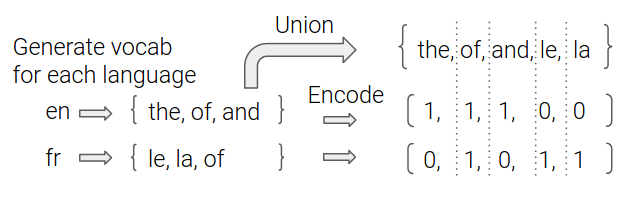
\includegraphics[width=0.9\textwidth]{img/temp/chung_language_vectors.png}
    \caption{Binary vector representations used for language clustering. Figure taken from \cite{chung_improving_2020}.}
    \label{fig:chung_vectors}
\end{figure}

Their method works by clustering similar languages together and then merging the cluster-level vocabularies. To cluster the languages using the k-means algorithm, it is necessary to define an Euclidean vector space with each language having a representative vector (\autoref{fig:chung_vectors}). To this end, the authors first train equally sized vocabularies $V^l$ for each language separately using the Unigram LM method. Then they create a merged vocabulary $V^L$ by taking the union of the vocabularies $V^l$. Then, to produce a language vector $\vec{v}^l$ for each language $l$, the presence of each subword $V^L_i$ is checked in the language-specific $V^l$ and the value is set to 1 if the subword is present and 0 otherwise. \xxx{this seems to be overly complicated explanation}

\begin{equation}
    \vec{v}^l_i = \begin{cases}
        1 & \text{if } V^L_i \in V^l \\
        0 & \text{otherwise}
    \end{cases}
\end{equation}

With the languages represented as vectors, the k-means algorithm can be used to cluster them. The authors use the cosine distance as the distance metric 
% (or equivalently: they normalize the language vectors to have a length 1 before clustering).
With 104 languages in total, the number of clusters is set to 8. The choice of $k$ is determined empirically by running a set of preliminary experiments and comparing the results on a multilingual question-answering benchmark. The resulting clusters are shown in \autoref{fig:chung_clusters}.

After the languages are clustered, the cluster-specific vocabularies are trained using the Unigram LM algorithm on the union of the corpora of the languages in the cluster. The size of each cluster-specific vocabulary is proportional to the size of the union of the individual (monolingual) vocabularies in the cluster. This means that more languages in a cluster lead to a larger vocabulary size assigned but also if the languages share tokens, this overlap decreases the vocabulary size. The final vocabulary is then constructed by simply taking the union over the cluster vocabularies.

\begin{figure}[ht]
    \centering
    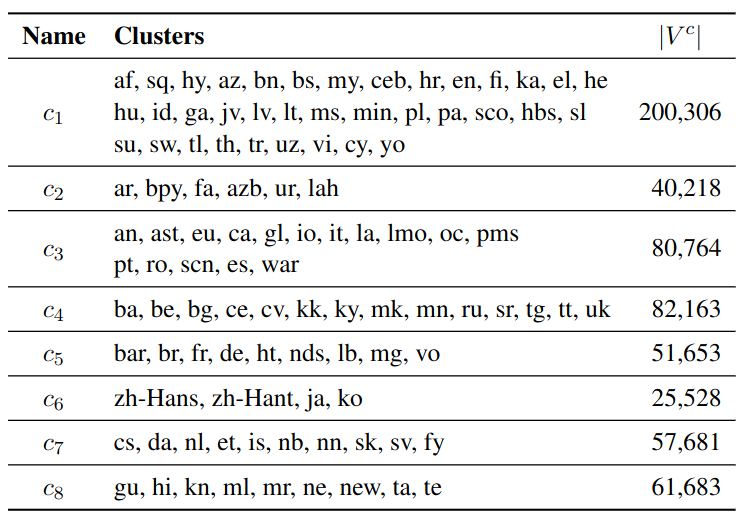
\includegraphics[width=0.8\textwidth]{img/temp/chung_clusters.png}
    \caption{Clusters of languages used in \cite{chung_improving_2020}. The clusters are numbered from 0 to 7. Figure taken from \cite{chung_improving_2020}.}
    \label{fig:chung_clusters}
\end{figure}

The final vocabulary is then compared to the standard recipe of training a Unigram LM vocabulary on a joint corpus\footnote{The authors do not define what they mean by following the "standard recipe". Based on the related work the authors replicate closely (mBERT and XLM-R) and compare themselves to, we assume that the standard recipe is training a Unigram LM tokenizer on the pretraining data after the exponential subsampling described in \ref{sec:data_scope}. The authors do mention using the sampling factor $\alpha=0.7$ for the pretraining data in the Appendix.}. Because the proposed clustering method does not have a way of controlling the size of the final vocabulary as taking the union inadvertently leads to some tokens being merged, the authors compare the vocabularies by first following the clustering method and arriving at a 488k subword vocabulary. Then the standard method is followed to train a vocabulary of the same size.

The authors evaluate the vocabularies intrinsically - by examining the average number of tokens per sentence, out-of-vocabulary rate and vocabulary overlap using the Wasserstein-1 distance.
By computing the average number of tokens per sentence for the whole corpus and for each language separately, the authors show that their method leads to a smaller average number of tokens per sentence for the whole corpus and further show that the improvements are more prominent for the low-resource languages. The authors also show that the out-of-vocabulary rate is lower for the language-clustered vocabulary, again the largest reductions in the OOV rate are in the low-resource and rare-script languages. Finally, the authors show on four selected languages that the language-clustered vocabulary leads to a smaller Wasserstein-1 distance between two similar languages and at the same time larger distance between two linguistically different languages.
\tomasz{Maybe write a sentence or two on using Wasserstein-1 distance for lang similarity.}

The clustered vocabulary is then used to train a smaller and bigger multilingual masked language model and evaluated on three distinct, multilingual tasks (question answering, natural language inference and named entity recognition). The baselines selected are the original mBERT model, XLM-R model and a smaller reproduction of XLM-R with an increased vocabulary size to match the parameter size of the introduced model. The authors show improvements for the smaller model on all three tasks over their baseline reproduction. Then they show the improvements in QA and NER tasks for the bigger model over the XLM-R and mBERT baselines. 

% The authors propose a new multilingual tokenization method. The vocabulary is constructed by clustering languages, applying SentencePiece to each cluster and merging the vocabularies together.
% The clustering is done by comparing similarity between monolingual vocabularies (NOT taking frequency of tokens into account - that is done in Liang et al 2023). Target vocabulary size for each cluster is proportional to the size of the union of the individual (monolingual) vocabularies in the cluster. The final vocabulary is simply union over the cluster vocabs (how do they ensure the target size for the whole vocab?)
% Intrinsic evaluation of the alternative vocabularies is done by computing the empirical distributions of the languages using Wasserstein-1 distance. The metric is used to compare the tokenizers and to prove that in the new approach, there is a smaller distance in the similar languages and at the same time bigger distance in the linguistically different languages. They also show that the Chinese and Arabic scripts is now in a larger share of the vocabulary.
% To analyze the “vocabulary allocation” they use a reformulation of description length for tokenizers = description length is equivalent to the the vocabulary size, and the number of integers of the encoded or tokenized input data. When comparing two tokenizers with the same vocabulary size, this is equivalent to comparing the average number of tokens per sentence. Caveat: there might be tradeoff with the out of vocabulary rate. They propose DL as a proxy metric to compare vocabularies.
% this work, we introduce a novel procedure for multilingual vocabulary generation that combines the separately trained vocabularies of several automatically derived language clusters, thus balancing the trade-off between cross-lingual subword sharing and language-specific vocabularies. Our experiments show improvements across languages on key multilingual benchmark tasks TYDI QA (+2.9 F1), XNLI (+2.1\%), and WikiAnn NER (+2.8 F1) and factor of 8 reduction in out-of-vocabulary rate, all without increasing the size of the model or data.
% Notes
% Because these algorithms look at overall subword frequencies in the combined multilingual corpus, they may learn suboptimal decompositions for low-resource languages that happen to have character combinations that resemble subwords of high-resources languages.
% subwords in common scripts like Latin and Cyrillic have a higher chance of selection since their counts are combined across a large number of languages (Wu and Dredze, 2019)
% subword sharing is not the principal reason for the effectiveness of multilingual models K et al. (2020)
% Ideas:

% - This still does not seem to solve the problem with cross-lingual sharing of wrong tokens such as “a” (conj in cs vs prep in eng)
% - Can we do the clustering better so that the languages are clustered according to the  downstream performance rather than hand-picked similarity metric between langs?

\subsection{Determining vocabulary capacity for each language}
\label{sec:zheng}

In the paper \Citetitle{zheng_allocating_2021}, \citeauthor{zheng_allocating_2021} propose a method for determining the optimal vocabulary capacity for each language in a multilingual model. Further, they propose a method for constructing a multilingual vocabulary by combining monolingual vocabularies so that the optimal capacity is achieved for each language. In the second part of the paper, the authors propose a method for accelerating the training of the model with the increased vocabulary size, which is out of the scope of this thesis.

% % - they observe that multilignual models do have a larger vocabulary than monolingual models (30k to 60k vs 250k). Still it is 2.5k per language on average in xlm-r
% - they consider each language separately and calculate the optimal vocabulary size for each language
% - using subword segmentation algorithms like BPE or unigram language model → they select subword tokens shared across languages with the same script and have lower chance to select language-specific subword units


To determine the optimal vocabulary capacity for each language, the authors propose a metric called \textit{average log probability} (ALP). 

$$
ALP(\mathcal{D}_i, V) = \frac{1}{|\mathcal{D}_i|} \sum_{j=1}^{|\mathcal{D}_i|} \sum_{k=1}^{|s_j|} \log(p_{uni}(s^k_{j}))
$$

where $\mathcal{D}_i$ is the monolingual corpus of language $i$, $V$ is the vocabulary and $p_{uni}(s^k_{j})$ is the unigram probability of the $k$-th token in the $j$-th sentence. The authors show that the average log probability positively correlates with the downstream task performance on a series of experiments with four distinct languages. They show this correlation by training a series of tokenizers with increasing vocabulary size. Then they measure the ALP on these tokenizers, pretrain monolingual models for every vocabulary size and every language and evaluate them on two word-level classification tasks. For illustration, we show the correlation between ALP and F1 score for the NER task in Figure \ref{fig:alp_vs_NER}. 

% show figure 2 and 3 
% \begin{figure}[h]
%     \centering
%     \begin{minipage}{0.45\textwidth}
%         \centering
%         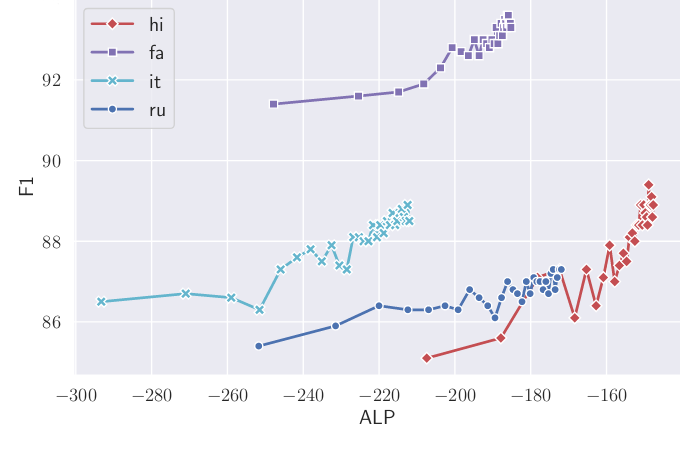
\includegraphics[width=\textwidth]{img/temp/alp_vs_NER.png}
%         \caption{F1 score on NER task with different vocabularies versus their ALP on the monolingual corpus. Figure taken from \cite{zheng_allocating_2021}}
%         \label{fig:image1}
%     \end{minipage}\hfill
%     \begin{minipage}{0.45\textwidth}
%         \centering
%         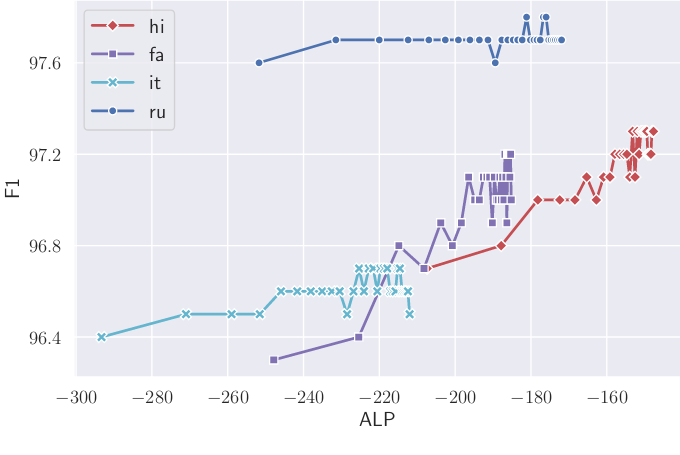
\includegraphics[width=\textwidth]{img/temp/alp_vs_POS.png}
%         % \caption{F1 score on POS task with different vocabularies versus their ALP on the monolingual corpus. Figure taken from \cite{zheng_allocating_2021}}
%         \label{fig:image2}
%     \end{minipage}
% \end{figure}

\begin{figure}[h]
    \centering
    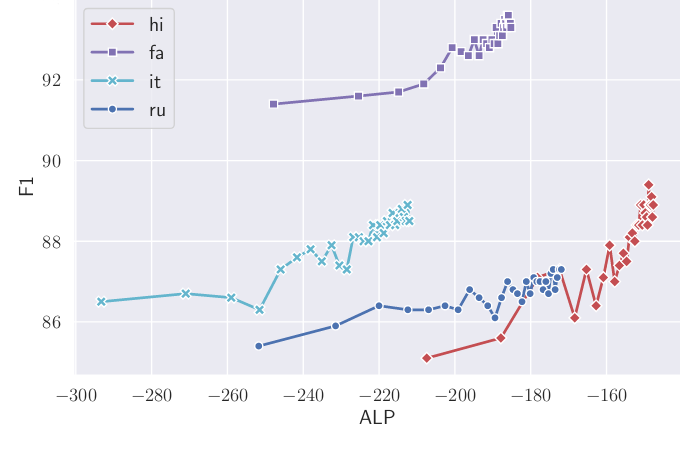
\includegraphics[width=0.65\textwidth]{img/temp/alp_vs_NER.png}
    \caption{F1 score on NER task with different vocabularies versus their ALP on the monolingual corpus. Figure taken from \cite{zheng_allocating_2021}}
    \label{fig:alp_vs_NER}
\end{figure}

Although the authors report that the vocabulary size itself is also a good predictor of downstream task performance, the authors argue that ALP correlates better with the downstream task performance and is therefore a better metric for determining the optimal vocabulary capacity.

%     - ALP correlates positively with downstream task performance
% - correlates better than only comparing vocabulary size
% - here they must compare pearson correlation because spearman would be the same for both - because ALP is a monotonic transformation of vocab size
% - but also for their usecase maximizing pearson is better because they then greedily select the vocab sizes based on ALP and then they want the metric to be linear with the downstream performance - so that the greedy selection is optimal

% This observation is in line with the research in machine translation \cite{gowda_finding_2020}. \xxx{maybe move this somewhere else and discuss the relevance for the MLMs, where we have much more training data than for the supervised MT} 

To efficiently allocate the tokenizer vocabulary, the authors hypothesize that the pretraining size of the corpora must be also taken into account. The reason is that for low-resource languages, it is better to allocate fewer tokens as the language model does not have enough data to learn robust representations for the low-frequency tokens. In the end, the authors propose a greedy vocabulary allocation algorithm \textsc{VoCap} that maximizes the following objective:

$$
\underset{t_1, \ldots, t_N}{\operatorname{argmax}} \sum_{i=1}^N q_i^\beta \operatorname{ALP}\left(D_i, V_{t_i}^i\right) \text { s.t. }\left|\bigcup_{i=1}^N V_{t_i}^i\right|=T
$$

Where $N$ is the number of languages, $q_i$ is the probability of sampling training instances from i-th language during pre-training (we describe the per-language sampling in \autoref{sec:data_sampling}), $\beta$ is a hyperparameter that controls the importance of the corpus size and $T$ is the total vocabulary capacity. 

The \textsc{VoCap} algorithm works by precomputing a series of tokenizer vocabularies with vocabulary sizes from 1\,000 to 50\,000 for every language and computing the ALP metric for each of them. Then it iteratively builds the final vocabulary by:

\begin{enumerate}
    \item Selecting the language with the highest potential ALP increase compared to the previous selected size.
    \item Taking the tokenizer with the increased vocabulary size for the selected language.
    \item Adding the tokenizer vocabulary to the final vocabulary.
\end{enumerate}

After reaching the target size, the algorithm halts and returns the vocabulary constructed by the iterative merging. The algorithm is shown in \autoref{alg:vocab_allocation}.

\begin{figure}[ht]
    \centering
    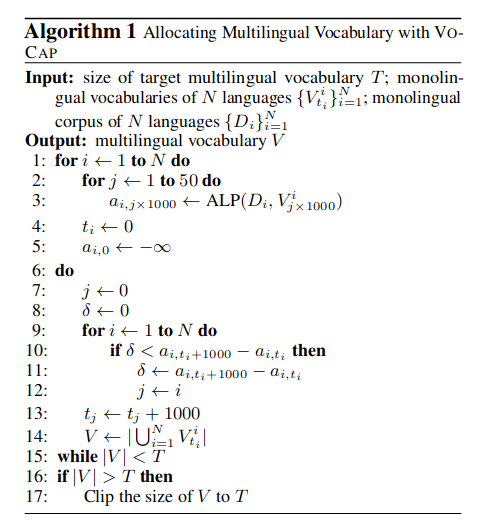
\includegraphics[width=0.8\textwidth]{img/temp/vocap_algo.png}
    \caption{\textsc{VoCap} algorithm pseudocode \cite{zheng_allocating_2021}. Figure taken from \cite{zheng_allocating_2021}.}
    \label{alg:vocab_allocation}
\end{figure}

With the \textsc{VoCap} algorithm, \Citeauthor{zheng_allocating_2021} then create new tokenizers with vocabulary sizes 250\,000 and 500\,000 on a multilingual corpus with 86 languages. The authors compare the performance of the \textsc{VoCap} tokenizers with baseline tokenizers trained directly on the multilingual corpus. The multilingual corpus is again subsampled before the standard tokenizer training following \citet{devlin_bert_2019,lample_cross-lingual_2019} with an exponential smoothing factor of $\alpha=0.7$.

The standard and \textsc{VoCap} tokenizers are compared using the ALP metric. The results are shown in \autoref{fig:alp_improvement}. The authors show that the \textsc{VoCap} tokenizers improve the ALP metric for the 500\,000 vocabulary size over the baseline across all languages. The improvement is more prominent for low-resource and mid-resource languages compared to high-resource languages. At the same time the difference between the standard tokenizers with vocabulary sizes 250\,000 and 500\,000 is negligible.

\begin{figure}
    \centering
    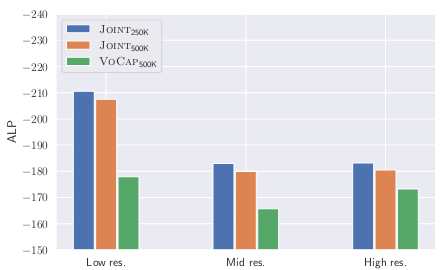
\includegraphics[width=0.8\textwidth]{img/temp/alp_improvement.png}
    \caption{ALP improvement of \textsc{VoCap} tokenizers over the standard tokenizers with vocabulary sizes 250\,000 and 500\,000. Figure taken from \cite{zheng_allocating_2021}.}
    \label{fig:alp_improvement}
\end{figure}

To validate these results, the authors then pretrain masked language models using the standard and \textsc{VoCap} tokenizers and conduct experiments on tasks from the XTREME benchmark \cite{hu_xtreme_nodate}. The comparison is done on natural language inference, paraphrase identification, part of speech tagging, named entity recognition and question answering. The averaged results over all tasks suggest that the \textsc{VoCap} tokenizers outperform the standard tokenizers by 0.4 percentage points for the 250\,000 vocabulary size and 1.7 percentage points for the increased 500\,000 vocabulary size. When investigating further the results for XNLI and NER, the authors show that improvements are gained in the low-resource and mid-resource languages. This is consistent with the ALP improvement results.

% With the \textsc{VoCap} algorithm \Citeauthor{zheng_allocating_2021} then create new tokenizers with sizes 250k and 500k and show that for larger dictionaries (500k vocabulary size) their method outperforms the standard method of training a joint vocabulary on the union of the corpora. 


\subsection{Combination of methods for scaling the vocabulary size}

In the paper \textit{XLM-V: Overcoming the Vocabulary Bottleneck in Multilingual Masked Language Models}, \citeauthor{liang_xlm-v_2023} introduce a new multilingual language model with a 1M token vocabulary. To create this large vocabulary, the authors propose a new tokenization method by combining the two methods described in the previous sections \ref{sec:chung} and \ref{sec:zheng}. 

% In this subsection, we describe our method for constructing multilingual vocabularies. At a high level, we (1) train individual monolingual sentencepiece models (SPM) for each language in our dataset using the Unigram Language Model (ULM) algorithm (Kudo and Richardson, 2018), (2) use the per-language vocabularies to construct lexical representation vectors for each language, (3) cluster the lexical representation vectors using K-Means, assign vocabulary capacities for each cluster using the ALP, and then construct per-cluster vocabularies using the ULM algorithm, and (4) create the final multilingual vocabulary by taking the union of the vocabularies for each cluster.

The proposed method consists of the following steps: (1) training monolingual tokenizers for each language using Unigram LM, (2) computing language vectors using negative log probability of the tokens, (3) finding a clustering of the languages with the k-means algorithm using the language vectors, (4) finding an appropriate vocabulary size for each cluster using the ALP from \citet{zheng_allocating_2021}, (5) training a tokenizer for each cluster using Unigram LM and (6) combining the tokenizers into a single multilingual tokenizer.

As we can see, the overall method is similar to \citet{chung_improving_2020} with small adjustments. More concretely, the authors train larger monolingual Sentencepiece Unigram tokenizers in the first step, use a different method for computing the language vectors in the second step and use the ALP metric for finding the appropriate vocabulary sizes in the fourth step. We now describe each altered step in more detail.

For training the monolingual tokenizers, the authors suggest using a larger vocabulary size of 30\,000 instead of 8\,000 used in \citet{chung_improving_2020}.

\begin{figure}[ht]
    \centering
    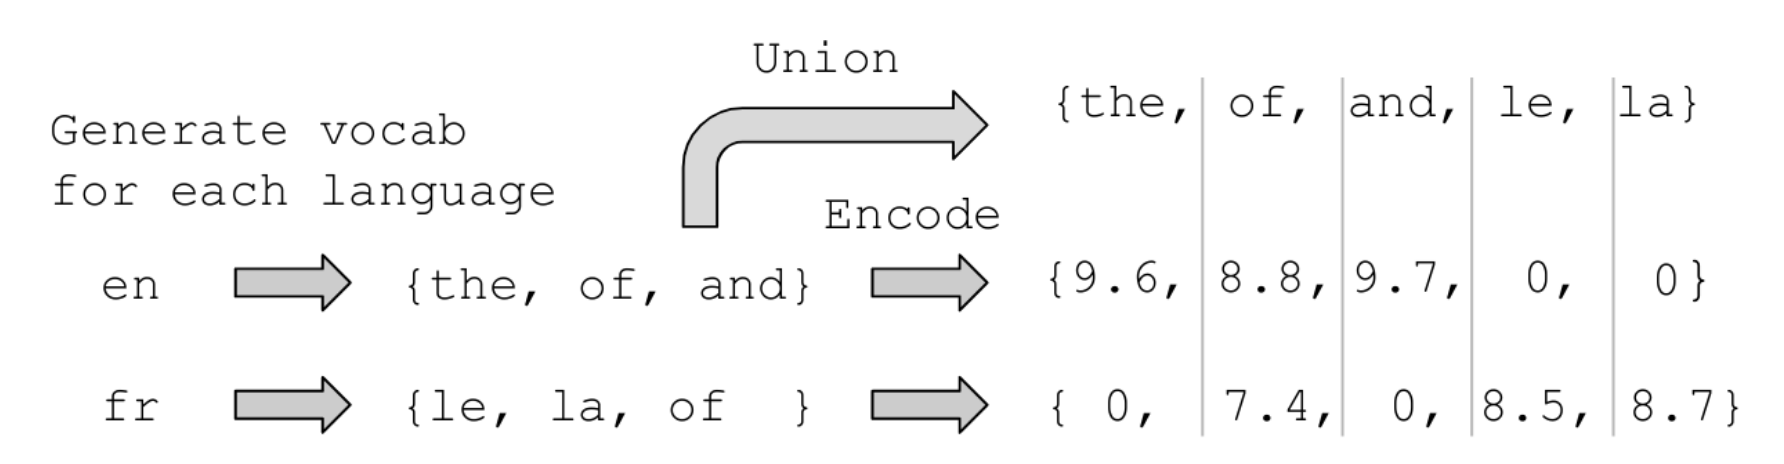
\includegraphics[width=0.9\textwidth]{img/temp/liang_language_vectors.png}
    \caption{Negative log probability vector representations used for language clustering. Compare to \autoref{fig:chung_vectors}. Figure taken from \cite{liang_xlm-v_2023}.}
    \label{fig:liang_vectors}
\end{figure}

The language vectors in \citet{chung_improving_2020} are binary with 1 corresponding to each subword present in the vocabulary of a given language. In contrast, \citet{liang_xlm-v_2023} propose to use the negative log probability of the subwords as the language vectors (see \autoref{fig:liang_vectors}). The logits are the output of the Unigram LM tokenization method as explained in \autoref{sec:unigram}. The authors argue that "weighting each token by its likelihood better represents the lexical fingerprint of a language".

Lastly, the authors argue that the method of \citet{chung_improving_2020} assigns deficient vocabulary sizes to some of the clusters, pointing out an example of a cluster containing Chinese and Japanese with a capacity of 28,593 tokens. The authors propose to use the ALP to allocate appropriate vocabulary sizes to each cluster. The exact method is unclear from the paper but to the best of our understanding, the method followed by the authors was to use the publicly available code and monolingual tokenizers from \citet{zheng_allocating_2021} and re-run the \textsc{VoCap} algorithm on their CC100 data instead of Wikipedia data. In this way, the authors obtained the optimized vocabulary sizes for the CC100 dataset for each language covered by \citet{zheng_allocating_2021}. Any language that was not included in the public implementation of \textsc{VoCap} was set to a fixed size of 2000 vocabulary size. The optimized vocabulary sizes for each language were then summed according to the cluster assignments to get the cluster vocabulary sizes. To achieve a specified target vocabulary size (500k, 1M, 1.5M, 2M), the authors then take the cluster vocabulary sizes and rescale them so that the sum equals the target size. As noted in \autoref{sec:chung}, the union of the vocabularies is not guaranteed to be equal to the target size because of the overlapping tokens between the cluster vocabularies. The authors report that the 1M vocabulary has an actual size of 901\,629 tokens.

After creating the vocabulary, the authors then train a large multilingual masked language model based on XLM-R following \citet{conneau_unsupervised_2020}. 

They run a shorter preliminary training with differently sized vocabularies (1M and 1.5M) and compare the performance of their proposed method to the original clustering method by \citet{chung_improving_2020} scaled to 1M vocabulary size and XLM-R with the original tokenization method scaled to 1M vocabulary size. They compare the results on the XNLI task and show that their method outperforms the other two methods by 1.11 and 1.34 percentage points respectively. 

After the preliminary run, they fully train the final model with the 1M vocabulary size on 2.5TB of data and compare the performance to the original XLM-R model with 250k vocabulary size. They show that their model significantly outperforms the original XLM-R model on a variety of language understanding tasks.

% The authors motivate their method by stating that the original XLM-R vocabulary is 

% The authors motivate their method by stating that two core principles will be upheld: (1) the vocabularies can be improved by de-emphasizing token sharing between lexically different languages and (2) proper allocation of vocabulary capacity for individual languages. These two points refer to the clustering of the vocabulary and the vocabulary allocation methods described above.


\subsection{Other approaches}

Several other works propose different methods for tokenization. In the thesis, we focus on methods that propose novel tokenization methods. There are however different approaches for text representation that aim to improve the performance of multilingual language models. We briefly describe some of them in this section.

Instead of costly pretraining of new models, \citet{wang_improving_2019} propose to extend the vocabulary of mBERT with new tokens. By adding new tokens, they lower the out-of-vocabulary rate for selected languages and in turn, improve performance on a variety of tasks. 

One possible avenue for mitigating problems of tokenization is to get rid of tokenization altogether. \citet{clark_canine_2022,tay_charformer_2022,xue_byt5_2022} propose different methods for skipping the input tokenization step and modifying the Transformer architecture to effectively process byte sequences. As \citet{mielke_between_2021} notes, however, these methods come with their own sets of biases and limitations such as lower performance or higher computational demands. 

Another direction of research is focusing on the visual representation of characters and subwords \cite{rust_language_2023,salesky_robust_2021,mansimov_towards_2020}. For example, logographic languages encode semantics in the shapes of the logograms, which is a source of additional information not present in the Unicode representation of the characters. The visual text representation models are also more robust to spelling errors and other artifacts.

% - extending the vocabulary with new tokens
% - multiview tokenization
% - etc, go through my notes

% identify the gaps in the current research
% - No systematic comparison of the metrics
% - There are more simple baselines to try

\chapter{Method}
\label{chap:method}

% In this chapter, we discuss the methodology of the thesis. We motivate and specify the research question, state the hypothesis and the specify how we test it.

% Methodology

% what do we want to measure? The effects of tokenization over the languages, focus on the differences the methods make on low resource vs high resource and how this translates to downstream tasks.b

% - data sampling
%     - !! do data hodně vysvětlit, že u toknizerů používáme různá alpha ale u pretrainingu ne.

% - introduce the metrics
%     - obecně naše metriky předpokládají nějaký předem daný vocabulary budget, který chceme spravedlivě rozdělit
%     - CPT, AR, JSD
%         - k AR metrice: je to samozřejmě závislý na vocab size, ale měl bych to poznamenat
%         - výhoda AR oproti CPT - u čínštiny započítává jednotlivé znaky, což by u CPT nebylo vidět

%         - k JSD metrice: není zřejmé jestli chceme vyšší overlap nebo nižší

%     - interpretation of the metrics - CPT, AR high good, JSD not sure
%     - also mention UNK and alphabet size
% - kinds of experiments
%     - tokenizers only
%         - eg: training data size, alphabet size, data imbalance
%     - tokenizers + MLM training
%         - eg: Huggingface tokenizers, replications
    
% - introduce the evaluation procedure
%     - intrinsic evaluation
%         - overall metrics - why macro average over languages
%             - how to average JSD - all pairs
%         - per language metrics - why delta from some baseline, metrics are different for different languages so we need to normalize
%     - extrinsic evaluation
%         - in-language / cross-language
%             - overall - why macroaverage, per-language, how to do per-language in cross-lingual where there are pairs (we focus on target results)
%             - seeds, averaging, bootstrapping
            %     - on how to compute significance for the cross-lingual tasks
            %         - we want to compare the average over languages
            %         - we can use bootstrapping to compute the confidence intervals
            %             - for each language select a random seed and compute the average over these seeds
            %             - sample many times and compute the confidence intervals
%         - probing vs finetuningn
%             - vysvětlit proč jsou všechny experimenty probing a jak se to liší a proč jsme to vybrali
%         - tasks NLI, NER, POS tagging, ...
%     - correlation between intrinsic and extrinsic
%         - how to compute the correlation
%         - míra korelace závisí na tom, jak moc se liší experimenty. Když porovnáváme jen stejné experimenty, pak nám vyjde nízká

% \textbf{Q1:} How do subword tokenizers differ in overlap and allocation of learned vocabularies?
% \textbf{Q2:} Which properties of multilingual tokenizers affect the language model representation quality?
% \textbf{Q3:} What is the reason that the standard tokenizer training method does not work well in the multilingual setting? 
% \textbf{Q4:} What is the effect of using the reproduced methods on the representation of low-resource languages? And
% \textbf{Q5:} How do the reproduced methods compare to the standard method of training the tokenizer on balanced and unbalanced joint corpus?


In this chapter, we introduce the methodology for experiments conducted in this thesis. We introduce the important data sampling method utilized in \citet{devlin_bert_2019,conneau_unsupervised_2020} we use frequently for our experiments.
Then we introduce our proposed metrics for measuring the \textit{vocabulary allocation} and \textit{vocabulary overlap} of a tokenizer. 
We introduce the types of experiments we will conduct. 
\tomaszrep{Namely}{Overall,} we will train different tokenizers and evaluate them against our metrics.
\tomaszrep{Moreover,}{Subsequently,} we will also use the tokenizers to train masked language models to verify that our metrics are useful for assessing the tokenizer quality for use in language models. We will also describe in detail the evaluation procedures and all evaluation settings and tasks. 

% \xxx{TODO - WIP}
% In this chapter, we explain the methodology for experiments conducted in this thesis. We answer our research questions stated in the \autoref{chap:introduction} in the following manner. In the \autoref{sec:tokenizer_metrics}, we introduce metrics for measuring the quality of tokenizers. We use these metrics to investigate the differences between tokenizers (\textbf{Q1}, ). We then validate the usefulness of our metrics by training masked language models using the tokenizers and evaluating them on a set of downstream tasks to see whether are our metrics good predictors of the model performance. (\textbf{Q2}). Then we use our metrics on a more granular level and investigate the differences 


% For all experiments we use the CC100 dataset used in \citet{conneau_unsupervised_2020}. Using the data we create multilingual vocabularies with the same size of 120K unique tokens using different methods. We use intrinsic evaluation framework from \citet{limisiewicz_tokenization_2023} to evaluate the tokenizers. Then we use the tokenizers to train multilingual masked language models on the same data and evaluate them on the same set of downstream tasks. We compare the results of the intrinsic and extrinsic evaluation to see if the improvements in the intrinsic evaluation translate to improvements in the downstream tasks.

% In this thesis, we investigate the effect of tokenizer properties on multilingual language models. We define metrics that measure the properties of the tokenizers and then we define the method by which we assess how these properties affect the performance of the language models. At the same time we want to improve the performance of the multilingual language model for the low-resource languages as this was shown to be a problem in previous work \cite{rust_how_2021}. Therefore we use the metrics we define to assess the methods proposed to solve this problem. Furthermore we propose methods to improve the performance of the language models and evaluate them using the same metrics.


\section{Data sampling}
\label{sec:data_sampling}

% This subset of CC100 is then used for further experiments with vocabulary creation that will be described in the following sections.
% \xxx{TODO: describe the resampling method, compare different alphas used in the literature}
% For pretraining the models and training the tokenizers we do not use the full 10\% of the data. Because the data is heavily skewed towards the high-resource languages. Instead, we further subsample the data, following \citet{conneau_unsupervised_2020-1} to balance the number of lines per language. This is a standard practice followed by multiple independent authors \xxx{cite}. The empirical probability of sampling a line from language $l$ is given by:

% In the following chapters, we will reference often the balancing factor $\alpha$, here we defin

As explained in the previous chapters \tomasz{refer to specific chapter}, the training data available for each language differs significantly in the total size (counted as the number of lines). For training the multilingual language model and associated tokenizer, it is generally advised to address this data imbalance by oversampling the languages with a low amount of data available (low-resource languages) and undersample the languages with high amounts of data (high-resource languages). One possible balancing procedure proposed by \citet{devlin_bert_2019,conneau_unsupervised_2020} is parametrized by the exponent $\alpha$ which we will now describe.
\tomaszrep{In the following chapters, we will reference often the balancing factor $\alpha$. 
If not mentioned otherwise, we consider data balance in the \textbf{tokenizer} training data (not pretraining data for the model) implied by sampling with the $\alpha$ parameter.}{[confusing, the second sentence is reiterated clearer at the end of the section.]}

We assume we have $N$ monolingual corpora $C_l$ with languages $l \in L$. Each corpus with the language $l \in L$ has a different number of lines $N_l = |C_l|$. Then, the probability of sampling a line from the concatenation of all corpora $\cup_{l \in L} C_l$ is:

\begin{equation}
    p(l) = \frac{N_l}{\sum_{l' \in L} N_{l'}}
\end{equation}

% Where $N_l$ is the number of lines in the dataset for language $l$.

To ensure that the low-resource languages are not underrepresented in the training data, we modify this probability distribution using an exponential smoothing parameter $\alpha$:

\begin{equation}
    p'(l) = \frac{p(l)^\alpha}{\sum_{l' \in L} p(l')^\alpha}
\end{equation}

For $\alpha = 0.0$ we get a uniform distribution over the languages, for $\alpha = 1.0$ we get the original distribution. 

For pretraining the language models, we use $\alpha = 0.3$ as suggested by \citet{conneau_unsupervised_2020-1}. For training the tokenizers, we always specify the alpha as a parameter of the tokenizer training procedure. 

\section{Tokenizer metrics}
\label{sec:tokenizer_metrics}

% \xxx{lets write the motivation here and maybe move it to the background section later}  

% - motivation: we want to evaluate the tokenizers before costly pretraining
% - by comparing the tokenizers we can select the best one for pretraining
% - we can also use the metrics to study the effect of the hyperparameters and other factors on the tokenizer
% - We use the metrics throughout the thesis to measure the tokenizers
% - We can measure how the tokenizer output differs between languages
%     - Explain how to measure individual languages with the same tokenizer. Metric may be a function of the tokenizer and language coded hold out data

% - Why do we want to measure the tokenizers?
%     - we want to select the best tokenizer for pretraining
%     - how do the tokenizers differ?
%         - overlap between languages - can be beneficial for some tasks (ner) but detrimental for others (pos)
%         - how much do they split words? (Rust)
%         - how much do they split sentences? (Limisiewicz)
%             - too much splitting - the model needs to learn to reconstruct words
%             - too little splitting - there is not enough examples for the model to learn from (but maybe this is not a problem for masked LM, only for machine translation)
%         - we can also measure the compatiblity of the segmentations (Maronikolakis)
%         - vocabulary capacity per language
%             - are the languages represented equally in the vocabulary?
%             - this is hard because some languages need more tokens than others (Chinese vs English)

% - how to measure tokenizers
%     - we want to measure the per-language and cross-lingual phenomena
%     - we therefore need to measure the tokenizers using language-coded data
%     - the basis for measurement will be the tokenization of the language-coded data and the empirical distribution of the tokens

%     - Average Rank - we want to measure how many tokens are used in the vocabulary - high frequency tokens are penalized because they move the average down
%         - another motivation - AR is similar to "the number of tokens needed to cover x% of the data" but it is non-parametric and includes the information about the distribution of the tokens
%     - Characters per Token - more characters = less ambiguity = better
%         - similar to word fertility, equivalent to tokens per sentence
%             - tokens per sentence used in Chung (they call it description length), Liang
%         - usable also in the langugaes without spaces
%     - of course both measures depend on the langugage

%     - interesting: ALP === entropy * avg_sequence_length

%     - overlap - what is the overlap between two languages
%         - we can look at the number of tokens that are shared between the languages but this is not that informative because these tokens might be very rare
%             - Wu and Dredze did this
%         - better is to look at the distributions of the tokens in each language and measure the similarity
%         - we can use the Jensen-Shannon divergence to measure the similarity of the distributions
%         - Chung used the Wasserstein distance but this is a distance function defined between probability distributions on a given metric space. (probability measures). We do not see how to interpret the token distribution as a probability measure and Chung does not discuss this

In this section we introduce the metrics that we use to evaluate the tokenizers. By measuring the tokenizers we would like to explore two questions. First, we would like to analyse how the tokenizers differ between each other. How granular is the segmentation given an example text? And how much are the tokens shared between the languages? Second, using the observed differences between tokenizers, we would like to analyse how they influence the multilingual language models, that are trained using the tokenizers. We will describe the methodology for measuring the influences in the following sections \xxx{ref}.

When assessing the multilingual tokenizers, we also want to focus not only on the overall properties but also investigate the quality of tokenization for the individual languages. This gives us a better understanding of the tokenizers and allows us to compare the tokenizers with each other given a target language. For this purpose, we will use monolingual evaluation corpora for each language. The metrics we define will be therefore functions of the tokenizer $\tau$ and the corpus $C_l$ with the selected language $l$. 

We introduce three metrics - average rank, characters per token and Jensen-Shannon divergence. The first two metrics aim to measure the "vocabulary allocation" of the tokenizer --- the degree to which is the given language represented in the vocabulary. The third metric measures the "vocabulary overlap" between a given pair of languages --- the degree of token sharing between two languages.

% Later, in \autoref{sec:metric_comparison}, we compare our metrics with the metrics used in the literature.

To define the metrics formally, we use the following notation \cite{zouhar_tokenization_2023}. Let $\Sigma$ be a set of characters we call the alphabet. In our context, the alphabet is the set of all valid Unicode characters. We call a string $\sigma \in \Sigma^*$ a line \tomasz{wait, what is $\Sigma^*$? How is it different from $\Sigma$?}. Finally, we call a multiset of lines $C_l = \{ \sigma_1, \ldots, \sigma_{N_l} \} \subset \Sigma^*$ a corpus of size $N_l$. The $l \in L$ denotes a language of the corpus from a set of languages $L$. Next, we denote the set $V_\tau \subset \Sigma^*$ as the vocabulary of a tokenizer $\tau$. The tokenizer $\tau: \Sigma^* \rightarrow V_\tau^*$ is a mapping from a line $\sigma \in \Sigma^*$ to a sequence of tokens $\tau(\sigma) \in V_\tau^*$. We denote the number of tokens in a sequence $s$ as $|s|$. Finally, we denote the number of occurrences of a token $v \in V_\tau$ in a corpus $C_l$ as $\textrm{cnt}(v, C_l)$.
\xxx{TODO: Check the notation}
% For each metric we will provide motivation and comparison with similar metrics used in the literature. 

% \xxx{mention the vocabulary allocation and vocabulary overlap}
\xxx{TODO: add UNK rate?!}

\subsection{Characters per token}

\begin{figure}[h]
    \centering
    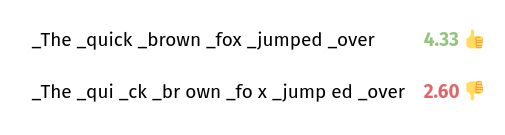
\includegraphics[width=0.6\textwidth]{img/temp/cpt_example.png}
    \caption{Example of CPT metric.}
    \label{fig:cpt_example}
\end{figure}

The first metric we propose is the average number of characters per token (CPT). The motivation for this metric is that we want to measure how granular the tokenization for a given language is. If the tokenizer splits the words into many tokens, the average number of characters per token will be low. On the other hand, if the tokenizer does not split the words, the average number of characters per token will be high. We hypothesize, that longer tokens are better for the language models, because they potentially carry more meaning. The extreme case of this metric is the character-level tokenization, where the average number of characters per token is 1. In this case the model would need to learn to reconstruct the words from the characters.

The metric is defined as follows. Given a tokenizer $\tau$ and a language corpus $C_l$, we first tokenize the corpus using the tokenizer $\tau$. Then we compute the average number of characters per token in the tokenized corpus:

\begin{equation}
    CPT(\tau, C_l) = \frac{\sum_{s \in C_l}|s|}{\sum_{s \in C_l}|\tau(s)|}
\end{equation}

where $|s|$ is the number of characters in the sentence $s \in C_l$ and $|\tau(s)|$ is the number of tokens in the tokenized sentence. The metric is illustrated in Figure \ref{fig:cpt_example}.

The CPT metric is connected to the \textit{average tokenized length} (or sequence length, or description length) metric used in \citet{chung_improving_2020,liang_xlm-v_2023}. 
These works suggest using the metric to compare whether one tokenizer splits a selected low-resource language into more tokens compared to another tokenizer. The average tokenized length is defined as the average number of tokens per sentence: 

\begin{equation}
\label{eq:tl_def}
    TL(\tau, C_l) = \frac{\sum_{s \in C_l}|\tau(s)|}{|C_l|}
\end{equation}

Where $C_l = {s_1, ..., s_{|C_l|}}$ from the language $l$ and $\tau$ is the tokenizer.

The tokenized length can be expressed as the product of the reciprocal of CPT metric and the average sentence length, which is corpus-specific and not dependent on the tokenizer:
\begin{equation}
\label{eq:tl}
    CPT(\tau, C_l)^{-1} \cdot \frac{\sum_{s \in C_l}|s|}{|C_l|} = \frac{\sum_{s \in C_l}|\tau(s)|}{\sum_{s \in C_l}|s|} \cdot \frac{\sum_{s \in C_l}|s|}{|C_l|} = \frac{\sum_{s \in C_l}|s|}{|C_l|} = TL(\tau, C_l)
\end{equation}

Even though the metrics are equivalent, we use the CPT metric instead of the average tokenized length because we believe it is more intuitive (higher CPT is better) and it is easier to interpret thanks to the lower bound of 1 character per token.

CPT is also similar to another metric used in the literature --- the word fertility metric used in \citet{rust_how_2021}. The word fertility is defined as the average number of tokens per word. We can see that the same argument as in \autoref{eq:tl} can be made about fertility and CPT. If we consider a corpus-specific constant "average number of characters per word", we see that fertility and CPT are proportional. The fertility metric has been shown to correlate with downstream performance and therefore seems to be a good metric. The downside of this metric is that it is not language-agnostic because it is not defined for languages without word delimiters such as Chinese or Thai.

\subsection{Average rank}

\begin{figure}[h]
    \centering
    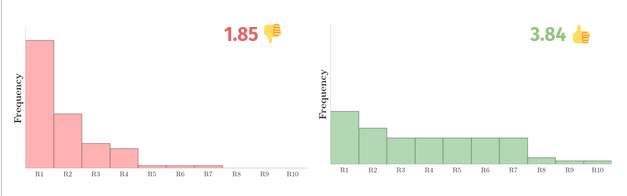
\includegraphics[width=0.6\textwidth]{img/temp/ar_example.png}
    \caption{Example of AR metric.}
    \label{fig:ar_example}
\end{figure}

Another metric we use for comparing the tokenizers is Average Rank (AR). The motivation for this metric is that we want to measure how many tokens are effectively used in the vocabulary for representing the corpus. Each language will have some amount of tokens dedicated to it in the vocabulary and our goal is to measure this allocation. We also want to take into account how frequently are these tokens used. We hypothesize that very frequent and very rare tokens are not as useful for the language models as the high-frequency tokens might be too ambiguous and low-frequency tokens might not have enough training examples to learn from \cite{gowda_finding_2020}. We therefore propose to measure the average rank (the position of the token sorted by frequency) of tokens \tomaszrep{needed to cover a monolingual corpus, weighted by their probability.}{in the empirical probability distribution over a monolingual corpus.}
% Here one metric suggestion could be something along the lines of "number of tokens from vocabulary of $\tau$ needed to cover the 95/98/100\% of the corpus". That metric would work but the downside is that we do not know how to set the threshold. Moreover we would like the metric to reflect the shape of the distribution of the token coverage. We prefer a distribution that is more balanced. High-frequency tokens might be too ambiguous and low-frequency tokens might not have enough training examples to learn from \cite{gowda_finding_2020}. Therefore we propose a different metric that reflects both the vocabulary allocation and the uniformity of the token distribution. On top of that it is parameter-free.

Given a tokenizer $\tau$ and a language corpus $C_l$, we first tokenize the corpus using the tokenizer $\tau$. Then we compute the empirical probability of the tokens in the tokenized corpus.

\begin{equation}
    \hat{p}_{\tau(C_l)}(t) = \frac{count(t, \tau(C_l))}{\sum_{t' \in \tau(C_l)} count(t', \tau(C_l))}
\end{equation}

We sort the tokens by their probability and assign them ranks from 1 to $|V_\tau|$. The average rank is then the weighted average of the ranks of the tokens, where the weights are the probabilites of the tokens:

\begin{equation}
    AR(\tau, C_l) = \sum_{t \in V_\tau} rank(t, \tau(C_l)) \cdot \hat{p}_{\tau(C_l)}(t)
\end{equation}

The metric is illustrated in Figure \ref{fig:ar_example}. Higher AR signals that the vocabulary contains higher number of tokens used for tokenizing given language. Moreover with high AR we can expect that the tokens are distributed more uniformly.

\tomasz{I suggest creating a subsection here:}
Now, we would like to address how our \textit{average rank} compares to different metrics used in the literature. 

First, we examine the \textit{average log probability} (ALP) defined in \citet{zheng_allocating_2021}. This metric is proposed for the same purpose as our AR metric. It is also said to measure language-specific vocabulary capacity and the authors claim that it is "penalized by the subword units with low-frequency". Surprisingly, we can show that the ALP metric is equivalent to the product of negative entropy and average tokenized length.

Given a monolingual corpus composed of sentences $C_l = {s_1, ..., s_{|C_l|}}$ from the language $l$ and tokenized with $\tau$, the ALP is defined as follows \cite{zheng_allocating_2021}:

\begin{equation}
\label{eq:alp}
    ALP(\tau, C_l) = \frac{1}{|C_l|} \sum_{s \in C_l} \sum_{t \in s} \log p(t)
\end{equation}

Where $p(t) = \frac{\mathrm{cnt}(t)}{\sum_{t' \in V_\tau} \mathrm{cnt}(t')}$ is the empirical probability of token $t$ in the corpus $C_l$. 

% In plain words, we sum the log probabilities of all tokens in the corpus and divide by the number of sentences in the corpus.

We can simplify the formula \autoref{eq:alp} by observing that we add up the log token probabilities $\log p(t)$ repeatedly by summing over all sentences and all tokens in sentences. Consequently, the sum can be simply expressed in terms of token occurrence multiplied by the log token probability. We denote $V_\tau$ the set of all tokens in the tokenizer vocabulary $\tau$ and $\mathrm{cnt}(t)$ the number of occurrences of token $t$ in the corpus $C_l$. We can rewrite the ALP metric as follows:

\begin{equation}
    ALP(\tau, C_l) = \frac{1}{|C_l|} \sum_{t \in V_\tau} \mathrm{cnt}(t) \log p(t)
\end{equation}

From here we can derive the relationship between token length (\autoref{eq:tl_def}), information entropy and ALP metric as follows:

\begin{align}
ALP(\tau, C_l) &= \frac{1}{|C_l|} \sum_{t \in V_\tau} \mathrm{cnt}(t) \log p(t) \\
&= \frac{1}{|C_l|} \sum_{t \in V_\tau} \frac{\sum_{t' \in V_\tau} \mathrm{cnt}(t')}{\sum_{t' \in V_\tau} \mathrm{cnt}(t')} \mathrm{cnt}(t) \log p(t) \\
&= \frac{\sum_{t' \in V_\tau} \mathrm{cnt}(t')}{|C_l|} \sum_{t \in V_\tau} \frac{\mathrm{cnt}(t)}{\sum_{t' \in V_\tau} \mathrm{cnt}(t')} \log p(t) \\
&= \frac{\sum_{t' \in V_\tau} \mathrm{cnt}(t')}{|C_l|} \sum_{t \in V_\tau} p(t) \log p(t) \\
&= \frac{\sum_{s \in C_l}|\tau(s)|}{|C_l|} \sum_{t \in V_\tau} p(t) \log p(t) \label{eq:alp_entropy_last_step}\\
&= TL(\tau, C_l) \cdot (- H(p))
\end{align}

In step \ref{eq:alp_entropy_last_step} we express the total number of tokens in corpus $C_l$ by counting over all sentences $s \in C_l$ and summing the number of tokens in each sentence $|\tau(s)|$.

% By analysis of ALP we see that the metric is composed of two metrics that are already well defined. Strangely, the metrics are multiplied together even though the effects of the metrics go against each other. On one hand the lower the token length the better (lower tokenized sentence length means longer and more meaningful tokens), on the other hand arguably, the higher entropy the better (more uniform distribution is better than very unbalanced distribution). It is not clear why would we want to multiply these two metrics together. The authors do not provide this analysis and discussion. \xxx{now interpretaion occured to me: the best ALP is achieved when we have short tokens that are balanced. So actually it could be interesting. But still the authors do not provide this analysis.}

By examination of ALP, it becomes evident that the metric is a composition of two already well-established metrics. Interestingly, these metrics are multiplied together, even though they seem to be inversely related. On the one hand, shorter token lengths are generally considered to be better (as a shorter tokenized sentence length means longer and more meaningful tokens), while on the other, a higher entropy is often deemed more desirable (a more uniform distribution is preferable to a more skewed one). One interpretation could be that high ALP is achieved when the vocabulary consists of a large number of short tokens that are similarly useful (have a uniform distribution). The authors, unfortunately, do not provide an analysis or discussion to shed light on this aspect. \xxx{We also note that the two metrics have different units, if we would want to combine them, it would be useful to add some factor that would determine which of the two metrics we deem more important.}

In comparison to our average rank, ALP measures the number of used tokens and the uniformity of the distribution thanks to the entropy in the equation. On the other hand, the ALP metric is punished by the length of the tokens, which is counterintuitive. We therefore stick to our AR metric, which is more intuitive and does not suffer from this issue.


\subsubsection{Average rank and entropy}

Next, a natural question is what is the difference between average rank and information entropy. The entropy of the tokenized corpus is defined as follows:

\begin{equation}
    H(\tau, C_l) = - \sum_{t \in V_\tau} p(t) \log p(t)
\end{equation}

Recall that we define average rank as follows:

\begin{equation}
    AR(\tau, C_l) = \sum_{t \in V_\tau} rank(t) \cdot p(t)
\end{equation}

We see that entropy provides similar characteristics as AR in the sense that more uniform distributions result in higher entropy and more tokens dedicated to a language also result in higher entropy. As we can see, the formula for entropy and AR differ only in the sign and one of the multiplied terms. The sign is not important as we are only interested in the relative values of the metrics. The difference in the multiplied terms is that AR uses the rank of the token, while entropy uses the log probability of the token. 

To proceed with the analysis, we will assume that the tokens follow Zipf's distribution. This is a reasonable assumption for natural language data. The Zipf's distribution is defined as follows:

\begin{equation}
    p_{zipf}(t) = \frac{1}{rank(t) \cdot H_{|V_\tau|}}
\end{equation}

Where $H_{|V_\tau|}$ is the $|V_\tau|$-th harmonic number used as a normalization constant.

Taking the logarithm of $p_{zipf}(t)$, we get:

\begin{equation}
    \log p_{zipf}(t) = - \log rank(t) - \log H_{|V_\tau|}
\end{equation}

Now if we plug in the log probability of the token into the entropy formula and leave out the constant as we are interested only in the relative values with a fixed vocabulary size, we get:

\begin{equation}
    H(\tau, C_l) \propto \sum_{t \in V_\tau} p(t) \log rank(t)
\end{equation}

We see that under the Zipfian assumption, the entropy may be viewed as an "average log rank". We empirically check this by computing average rank, average log rank, and entropy the Figure \ref{fig:ar_alr_entropy}.

\begin{figure}
    \centering
    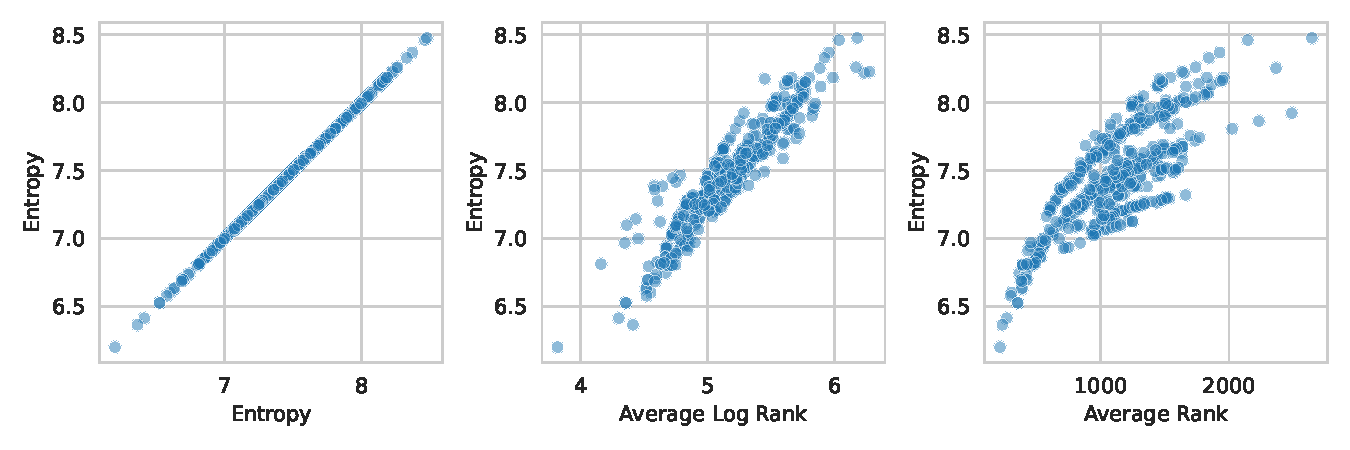
\includegraphics[width=0.9\textwidth]{figures/ar_alr_entropy.pdf}
    \caption{We compute the average rank, average log rank, and entropy for different tokenizers and languages. Then we plot each metric against entropy. We see that entropy and average log rank are similar, which supports our assumption that the tokens follow Zipf's distribution.}
    \label{fig:ar_alr_entropy}
\end{figure}

This provides us with an intuitive understanding of the difference between the two metrics. AR and entropy can be viewed as being related, with the difference being in their sensitivity to the rank of the tokens. AR, being directly related to rank, is more sensitive to changes in probability in lower-frequency tokens. This is because the weighted average used in AR is more affected by linear rank values than the logarithmic rank values used in entropy calculation.

\subsection{Jensen-Shannon Divergence}
\label{sec:jsd}

\begin{figure}[h]
    \centering
    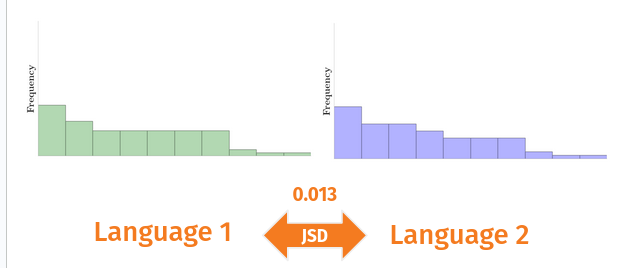
\includegraphics[width=0.5\textwidth]{img/temp/jsd_example.png}
    \caption{Jensen-Shannon Divergence \tomasz{cite the source: poster}}
    \label{fig:jsd_example}
\end{figure}

The Jensen-Shannon Divergence (JSD) is a metric that measures the similarity between two probability distributions. It is defined as follows:

\begin{equation}
    JSD(p, q) = \frac{1}{2} \cdot (KL(p||m) + KL(q||m))
\end{equation}

Where $m = \frac{1}{2} \cdot (p + q)$ is the midpoint distribution and $KL(p||q)$ is the Kullback-Leibler divergence. 

\begin{equation}
    KL(p||q) = \sum_{t \in V_\tau} p(t) \log \frac{p(t)}{q(t)}
\end{equation}

We will use JSD for the analysis of an overlap between two languages given a tokenizer. Tokenization of two monolingual corpora $C_{l_1}$ and $C_{l_2}$ with the same tokenizer $\tau$ will result in two probability distributions over the vocabulary $V_\tau$. We will denote these distributions as $\hat{p}_{\tau(C_{l_1})}$ and $\hat{p}_{\tau(C_{l_2})}$. 

Computing the JSD between the two distributions will result in a metric that measures how much the two distributions overlap. The JSD is a symmetric metric that is bounded between 0 and 1. Low JSD means that the two distributions are similar, high JSD means that the two distributions are different. 

Overlap in tokenization has been studied in \citet{wu_beto_2019}, although the metric used there was the absolute number of overlapping tokens. The benefit of using Jensen-Shannon divergence for measuring the vocabulary overlap is that the metric takes into account the occurrence of the shared tokens. This is important because some of the overlapping tokens may be for example infrequent emojis or other special tokens that do not carry much information about the language nor the actual overlap in more meaningful tokens.

\citet{chung_improving_2020} uses the Wasserstein distance (or the "earth mover's distance") to measure the overlap between two languages. We believe this is \tomaszrep{a mistake}{suboptimal} as the Wasserstein distance is defined for probability measures (probability distributions on a given metric space). The tokenizer vocabulary has no metric structure and the authors of the article do not specify how they define the metric on the vocabulary. It is therefore not suitable to use the Wasserstein distance for measuring the overlap between two tokenizers.

\subsection{Alphabet size and out-of-vocabulary tokens}

Among the metrics we propose, we also measure the alphabet size of the tokenizers defined as the number of tokens of length 1 in the vocabulary:

\begin{equation}
    \mathrm{Alphabet} = |\{t \in V_\tau, |t| = 1\}|
\end{equation}

We also measure the number of out-of-vocabulary (OOV) tokens in the corpus. The UNK token is a special token that used to represent all the tokens that are not present in the vocabulary $V_\tau$. We measure the number of UNK tokens in the corpus as follows:

\begin{equation}
    \mathrm{OOV} = \sum_{t \in \tau(C_l)} \mathbbm{1}_{t = \mathrm{<UNK>}}
\end{equation}

Where $\mathbbm{1}_{t = \mathrm{<UNK>}}$ is an indicator function that is 1 if the token is UNK and 0 otherwise. Because we use the same validation set for all the tokenizers, we can compare the number of OOV tokens directly between the tokenizers. Note that in the literature, the out-of-vocabulary tokens are measured as a OOV rate (number of OOV tokens divided by the total number of tokens in the corpus). We do not use this metric because the values of the OOV rate are small for the subword tokenizers and therefore slightly harder to compare.
\tomasz{I think OOV rate could be better because it's not sensitive to the size of the corpus. But if you already compute the abs. number then leave it.}

% Further, we will be mainly concerned with the tokenization of the training corpora $\tau(C_l)$ and the empirical distribution over the tokenizer vocabulary:

% \xxx{fix the equation once I settle on the notation. The denominator is wrong here}

% - test the tokenizer metrics, show correlation between CPT, AR and JSD -> downstream
%     - define the metricshe implementation}

% In \cite{limisiewicz_tokenization_2023} we have compared the Unigram LM and BPE tokenizers. We have found that generally, the BPE tokenizer performs better on the tokenizer intrinsic metrics and the downstream tasks. During the work on the thesis we have found that this finding might have been heavily influenced by the choice of the implementation of the Unigram LM training algorithm. In \cite{limisiewicz_tokenization_2023} we have used the Huggingface implementation of the tokenizers. In the later experiments we have used the Sentencepiece implementation. We have found that the Sentencepiece implementation produces tokenizers that close the gap in the intrinsic evaluation. We have therefore decided to use the Sentencepiece implementation for all experiments in this thesis.

% \xxx{add image}

% \xxx{TODO: add the other factors - co
%         - CPT
%         - AR
%         - JSD
%     - compare 4 tokenizers
%         - vanilla Unigram, vanilla BPE
%         - NoOverlap - to study the effect of the overlap
%         - TokMix - to ensure a uniform 
%     - experiments for 6 languages
%     - experiments for 20 languages

% \section{Investigating the influence of the tokenizer on the language model}

\section{Evaluation procedures}

In this section, we introduce the evaluation procedures that we use to evaluate the tokenizers. We first describe the types of experiments we do with the tokenizers. Then we explain the intrinsic evaluation procedure. Then we describe the extrinsic evaluation procedure.

\subsection{Types of experiments}

Generally, we can distinguish two types of experiments we do with the tokenizers we compare in this thesis. The first type of experiment is comparing different tokenizers to each other using the evaluation metrics we introduced in the previous section. For example, we can compare the Unigram LM tokenizer to the BPE tokenizer. To do this, we will train the tokenizers on the same training corpus and then evaluate them using the intrinsic evaluation metrics on validation sets \tomaszrep{from}{for} all the languages $L$. 

The second type of experiment is comparing different tokenizers on downstream tasks. For example, we can compare the Unigram LM tokenizer to the BPE tokenizer on the task of natural language understanding. To do this, we will train the tokenizers on the same training corpus and then use the tokenizers to train otherwise identical language models. Then we will evaluate the language models on \tomaszrep{the same validation sets from}{test[?] sets for} all the languages $L$. 

\subsection{Intrinsic evaluation}
\label{sec:intrinsic_evaluation}

For the intrinsic evaluation of a set of tokenizers, we compute the metrics we introduced in the previous section on the validation sets from all the languages $L$. We compute the metrics for each tokenizer and validation language separately. Then, we compare the per language metrics between the tokenizers. Because the metrics are generally different for different languages (for example the characters per token for Chinese will be always smaller than the characters per token for English), we will compare the relative differences between the tokenizers rather than the absolute values.

We will also compute the overall metrics for the whole set of languages $L$. We do this by averaging the metrics over all the languages. We use the macro average over languages, which means that we average the metrics for each language with the same weight. We use the macro average because we want to assess equally the \tomaszrep{improvements over}{impact on} the high-resource and low-resource languages. This is a choice we make to assess each language equally. Different weighting schemes might be more appropriate for different applications. Equal weighting across languages is also in line with how are multilingual models evaluated in the related work \cite{ruder_xtreme-r_2021}.

The JSD metric which measures the \textit{vocabulary overlap} is defined between a pair of languages, measuring the overlap between the two. We compute the overall overlap by considering the JSD values for all pairs \tomasz{of languages:} $l_1, l_2 \in L, l_1 \neq l_2$.

\subsection{Extrinsic evaluation}
\label{sec:extrinsic_evaluation}
%     - extrinsic evaluation
%         - in-language / cross-language
%             - overall - why macroaverage, per-language, how to do per-language in cross-lingual where there are pairs (we focus on target results)
%             - seeds, averaging, bootstrapping
            %     - on how to compute significance for the cross-lingual tasks
            %         - we want to compare the average over languages
            %         - we can use bootstrapping to compute the confidence intervals
            %             - for each language select a random seed and compute the average over these seeds
            %             - sample many times and compute the confidence intervals
%         - probing vs finetuningn
%             - vysvětlit proč jsou všechny experimenty probing a jak se to liší a proč jsme to vybrali
%         - tasks NLI, NER, POS tagging, ...
%     - correlation between intrinsic and extrinsic
%         - how to compute the correlation
%         - míra korelace závisí na tom, jak moc se liší experimenty. Když porovnáváme jen stejné experimenty, pak nám vyjde nízká

For the extrinsic evaluation of \tomaszrep{a set of}{} tokenizers, we compare the performance of \tomaszrep{a set of}{corresponding} language models that differ only in the tokenizers used.
\tomasz{The performance is compared}{We evaluate the performance} on a set of language understanding tasks.
Because the language models are identical except for the tokenizer used, the differences in the performance will be caused only by the differences in the tokenizers and random factors such as the weight initialization of the language models.

Concretely, given a set of tokenizers, we train \tomaszrep{a set of}{corresponding} masked language models with the same architecture and pretraining data.
 We then evaluate the models by training linear classifiers (probes) on top of the contextualized word embeddings produced by the language models. 
 For a given pretrained model, we train probes for each task-language combination utilizing training data in all languages given for the task.
 For each configuration, we train 3 random initializations of the probe with different seeds to acquire more stable results and an estimate of the variation. In total, $N_\mathrm{models} \times N_\mathrm{tasks} \times N_\mathrm{languages} \times N_\mathrm{seeds}$ probes are trained to compare the performance of the models for one experiment.

We use probing \cite{conneau_what_2018,belinkov_interpretability_2020,blevins_analyzing_2022} to evaluate the language modeling capability of the models. Instead of finetuning we freeze the base model and train only linear classifiers on top of the outputs of the base model. This approach allows us to evaluate the language modeling capability of the models without the influence of the finetuning procedure. 
\tomaszrep{We choose probing because it leads to less noisy results than finetuning.}{[I'm afraid it's false]}

% the noise could be caused by the smaller difference between pretraining data amount and the amount of data used for finetuning.

To evaluate a model $m$ on task $t$ and languages $t_L$, we will train probes $f_{m, t, l_\mathrm{src}}$ for each training (source) language $l_\mathrm{src} \in t_L$. Then the probe will be evaluated on the task test sets in languages $l_\mathrm{tgt} \in t_L$ using standard classification metric \tomaszrep{s used for the given task such as accuracy and the F1 score.}{ (in our case: accuracy or F1).} 
% full probe notation: $f_{m, t, l_\mathrm{src}}: \mathbb{R}^d \rightarrow \mathcal{D}_t$

% given model outputs $\vec{x} \in $, we can evaluate the performance of the probe on a given language $l_\mathrm{tgt}$ by computing the accuracy of the probe on the test set for the given language $l_\mathrm{tgt}$.

\subsubsection{Evaluation schemes}

We will distinguish between two evaluation schemes - in-language evaluation and cross-language \xxx{(cross-lingual?)} evaluation. 

The in-language performance of the model $m$ for task $t$ and a language $l$ will be computed by evaluating the probe $f_{m, t, l}$ on the test set for the same language $l$. 
The overall in-language performance of the model $m$ for task $t$ will be computed by averaging the in-language performance over all the languages $l \in t_L$. 

The cross-language performance of the model for task $t$ from the source language $l_\mathrm{src}$ to the target language $l_\mathrm{tgt}$ will be computed by evaluating the probe $f_{m, t, l_\mathrm{src}}$ on the test set for a different language $l_\mathrm{tgt} \neq l_\mathrm{src}$. 
The overall cross-language performance of the model $m$ for task $t$ will be computed by averaging the cross-language performance over all the language pairs $l_\mathrm{src}, l_\mathrm{tgt} \in t_L, l_\mathrm{src} \neq l_\mathrm{tgt}$.
Moreover, we will compute the cross-language performance per language $l$ of the model $m$ for task $t$ by averaging the cross-language performance over all the languages $l_\mathrm{src} \in t_L$ given a target language $l$.

When considering the results per language in both evaluation schemes, it is useful to consider only the relative differences between the models rather than absolute values. The performance of the models for a given language is influenced by eg. by the amount of training data available for the language. Therefore, when interpreting the results per language, we will choose a reference model and compute the relative difference between the performance of the reference model and the other models.

\subsubsection{Correlation between intrinsic and extrinsic evaluation}
\label{sec:correlation_intrinsic_extrinsic}

To support the claim that intrinsic evaluation is a good proxy for extrinsic evaluation, we will compute the correlation between intrinsic and extrinsic evaluation. Because the tokenizer metrics and model performance are influenced by the evaluation language as mentioned in the previous paragraph and in \autoref{sec:intrinsic_evaluation}, we center the tokenizer metrics and downstream task results by subtracting the mean for each language in the in-language setting or pair of languages in the cross-lingual setting. In both cases, means are computed across all tokenizers. We present Spearman’s correlation coefficient and the associated p-value.

\subsubsection{Variation estimation}

To account for the inherent randomness of the training procedure, we will train multiple probes for each configuration $(m, t, l)$. We will use 3 random seeds for each probe and report the average performance over the seeds. We will also report the standard deviation of the performance over the seeds. In the case of the summarized performances, we estimate the standard deviation using bootstrapping over the seeds.

Note that because for one tokenizer we pretrain only one model, as it is the most costly part of the experiment, we do not estimate the variance for the pretraining of the model.
\tomaszrep{We will interpret the results of the experiments with this fact in mind.}{[unnecessary]}


% For evaluating the language modeling capability of the models we use two techniques. First, we want to evaluate the performance of the models using finetuning on language understanding tasks. This approach is taken by the related work and it is the standard way of multilingual model evaluation. We use part of the XTREME benchmark, namely the Natural language inference, Part of Speech tagging and Named entity recognition tasks. For each task we finetune on every language and measure the performance on the development set. We do not apply any hyperparameter search apart from choosing a satisfactory learning rate and batch size for each task by running few short experiments. 

% Second, we also use probing \cite{conneau_what_2018,belinkov_interpretability_2020,blevins_analyzing_2022} to evaluate the language modeling capability of the models. We use the same tasks from XTREME benchmark, but instead of finetuning we freeze the base model and train only simple linear classifiers on top of the base model. This approach allows us to evaluate the language modeling capability of the models without the influence of the finetuning procedure. 


% \tomasz{Here, I would write section Extrinsic Evaluation. 
% With general description assesing tokenizer influnce on downstream tasks.
% Details should be provided in the next chapter: Experiments...}


\section{Evaluation on downstream tasks}

Here we present the downstream tasks we use in our paper \cite{limisiewicz_tokenization_2023}. For our further experiments, we use a subset of these tasks (POS, NER, NLI) that we have found to have different responses to the changes in the CPT, AR and JSD metrics.

\subsection{POS}

We use Part of Speech annotations from Universal Dependencies \cite{nivre_universal_2020}. The dataset is available for 17 languages analyzed by us (not covered: Swahili, Thai, Georgian). \tomasz{PROBLEM: You haven't introduced the list of languages yet!} Each word is assigned one of the 17 coarse POS tags.

\subsection{NER}

We use Wikiann dataset \cite{pan_cross-lingual_2017} consisting of Wikipedia articles with annotated named entities of three types: location, person, and organization in IOB2. Following XTREME, we use balanced data splits from \cite{rahimi_massively_2019}.

\subsection{Dependency labeling}

As in Part of Speech, we use Universal Dependencies \cite{nivre_universal_2020} for the dependency relation annotations. We use the largest UD treebank available for each language.
For each word, we predict one of the 37 universal relations to its head word. Because the relation is between two words, we use the concatenation of the two word representations along with their element-wise product as an input to the probe ($[h_{w1}; h_{w2}; h_{w1} \odot h_{w2}]$).

\subsection{NLI}

We use XNLI dataset \cite{conneau_xnli_2018} for Natural Language Inference. We train the linear classification probe on top of the concatenation of two sentence vectors and their element-wise product: $[h_{s1}; h_{s2}; h_{s1} \odot h_{s2}]$. We predict one of two relations between the first of sentences (called premise): contradicts, entails, or is neutral to the second sentence (called a hypothesis). We evaluate XNLI with the accuracy of classification.

XNLI contains data for 15 languages (not covered: te, ta, mr, he, ka).

\subsection{Sentence Retrieval}
We use up to 1,000 sentences aligned for pairs of languages from Tatoeba dataset \cite{artetxe_massively_2019}. For the pairs including English, we use the same sample as in XTREME data collection. For other pairs, we perform sampling ourselves. 

We compute the cosine similarity between sentence representations across languages and find the best alignment with the Hungarian algorithm\cite{kuhn_hungarian_1955}. We compute the accuracy as the number of correctly aligned sentences divided by the total number of sentences.


\section{Implementation Details}
\tomasz{IMO good place to dump all Appendi-worthy details.}

\subsection{Tokenizers}
\subsection{Model Pretraining}
\subsection{Probing}


\section{Reproducing the vocabulary balancing methods}
\label{sec:reproducing_the_vocabulary_balancing_methods}
% - replication of the previous balancing work
%     - the code is not available for Chung and Liang, for Zheng we reimplement even though the code is available
%     - therefore we follow all papers closely
%     - Chung
%         - reproductions of chung are available in the paper Overlap-based Vocabulary Generation Improves Cross-lingual Transfer Among Related Languages
%             - they do not replicate the results of Chung
%         - we run training with 8k vocab size, unigram, coverage 0.9995 (default in Sentencepiece) for each language
%             - this is specified in the paper
%             - we use 1M lines for each language which we have shown to be enough in preliminary experiments
%         - we compute the binary vectors for each language and normalize them to unit length
%         - we compute clusters using k-means, with k=4, 8, 12, 16, 20 (=all languages)
%         - train the tokenizers on the clusters
%             - target vocab size is 120k, again use Sentencepiece defaults
%             - to reach the vocab size we train also +10\%, +20\%, +30\% of the target size and then prune
%         - then we merge the tokenizers

%     - Liang
%         - we follow the same procedure as in Chung
%         - compute negative log-likelihoods for each token over the corpus and use the euclidean distance to compute the similarity
%         - but we use the sizes from Zheng

In this section, we describe our reproduction of the existing methods for balancing the low- and high- resource languages in the vocabulary. As the code for two out of three of the methods is not available, we follow and reimplement the original papers closely and describe the differences in our implementation.

The methods of \citet{chung_improving_2020} and \citet{liang_xlm-v_2023} follow a three step process: 1) grouping the languages into clusters by similarity, 2) running the Unigram LM tokenizer training on the clustered corpora and 3) combining the cluster-vocabularies into a single, multilingual vocabulary. Because of their similarity, we refer to the two as the clustering methods. The method of \citet{zheng_allocating_2021} works in two steps: 1) training the Unigram LM tokenizers for each language separately and 2) selecting the best vocabulary size for each language and combining the vocabularies into a single, multilingual vocabulary.

As we can see the methods share the last merging step and differ in the clustering approaches. We therefore describe the clustering approaches first, then we describe the Zheng method and finally we describe the merging step common for all methods.

\subsection{Reproducing the clustering methods}
% \tomasz{General remark: It's better to keep experiments definition (i.e. hypothesis statement and experiment overview.) separated from implementation details.
% The later are important bu shouldn't steal attention of the reader from the story.}

The first step for the Chung and Liang methods is to train monolingual Unigram LM tokenizers for each language $l$ from the set of 20 languages $L$. As specified in \citet{chung_improving_2020}, we use the default Sentencepiece settings. Namely, we use the Unigram LM model, character coverage of 99.95\%, number of seed sentencepieces is 1M. \xxx{add all parameters to appendix?}. 
For training the monolingual tokenizers, we use 1M lines for each language which we have shown to be enough in preliminary experiments \autoref{sec:data_size}. This choice also corresponds to the \citet{zheng_allocating_2021} method, which uses 1M lines for each language. The vocabulary size differs between Chung and Liang and so we train two sets of monolingual tokenizers, with 8k and 30k vocabulary sizes respectively.

We arrive at $|L|$ vocabularies $V^l$. Next, we take the union of all vocabularies $V^L = \bigcup_{l \in L} V^l$ and compute the "vector representation" $\vec{v}^l$ for each language $l$ as described in \autoref{sec:chung} and \autoref{sec:liang}. For Chung, we compute a binary vector of size $|V^L|$, where each element $\vec{v}^l_i$ is 1 if the token $i$ is in the vocabulary $V^l$ of language $l$ and 0 otherwise. For Liang, we compute a vector of size $|V^L|$, where each element $\vec{v}^l_i$ is the negative log-likelihood of the token $i$ in the language $l$ as computed by the Sentencepiece training algorithm. We set the log-likelihood of the tokens not in the vocabulary to 0 as inferred from the Figure 1 in \cite{liang_xlm-v_2023}. We discuss this choice in more detail in the discussion \autoref{sec:language_vectors}.

With the vector representations $\vec{v}^l$ we can cluster the languages into $k$ clusters $C^k$ using the k-means algorithm. We use the implementation from \texttt{scikit-learn} \cite{pedregosa_scikit-learn_2011} with the default parameters. \citet{chung_improving_2020} reports using the cosine distance for the k-means algorithm. We normalize the language representation vectors to unit length, to achieve the same effect. In the case of Liang, we stick to Euclidean distance as the authors do not mention using a different metric. We experiment with $k \in \{4, 8, 16, 20\}$. Note that $k=20$ corresponds to separating each language into a separate cluster which is similar to the method \textsc{TokMix} we introduce in \citet{limisiewicz_tokenization_2023} and \citet{zheng_allocating_2021} we replicate next.

Then, given a clustering of languages $C$, for each cluster $c_j \in C$ we create a new training corpus by concatenating all of the CC100 data belonging to the cluster\footnote{Because of computational constraints, we cap the total number of lines per cluster to 20M. If the cluster corpus exceeds the total number of lines, we subsample the available data with $\alpha=1.0$}. We run the Sentencepiece algorithm again on these clustered corpora to arrive at cluster-specific vocabularies $V^{c_j}$. The vocabulary size for each cluster is determined following the Chung and Liang methods. For both methods, we want to arrive at the final size of 120k tokens after merging the cluster-specific vocabularies. Therefore we need to determine the size of each cluster vocabulary $|V^{c_j}|$ such that $\sum_{j=1}^k |V^{c_j}| = 120k$. The Chung method sets the size of the cluster vocabulary to be proportional to the size of the union over the monolingual vocabularies $|\bigcup_{l \in c_j} V^l|$ to determine the size of each cluster vocabulary as follows:

\begin{equation}
    |V^{c_j}| = \frac{|\bigcup_{l \in c_j} V^l|}{\sum_{i=1}^k |\bigcup_{l' \in c_i} V^{l'}|} \cdot 120k
\end{equation}

The Liang method proposes to set the size of the cluster vocabulary to be proportional to the sum of the vocabulary allocations from \citet{zheng_allocating_2021} for the languages belonging to the cluster. We use the allocations we reproduce in \autoref{subsec:reproducing_vocap}.
\footnote{
    Here we slightly improve the methods of Chung and Liang. By following the original method as described above, the final size of the vocabulary will be lower than the target we set. This is because the cluster vocabularies $V^{c_j}$ will contain overlapping tokens and merging will remove these duplicates. This negative effect becomes larger with the increasing number of clusters $k$. Therefore, on top of training the prescribed cluster vocabulary of size $|V^{c_j}|$, we also train slightly larger vocabularies $V_q^{c_j'}$ of size $|V_q^{c_j}| = q|V^{c_j}|$ for $q = 1.1, 1.2, 1.3$. We then select the minimum $q$ that results in a vocabulary size of at least 120k tokens after merging the cluster vocabularies. After that, we trim the vocabulary if needed. This improvement is done to ensure the final vocabulary size is exactly 120k tokens and the comparison between the methods is fair.
}

After the tokenizers are trained, we merge the vocabularies using the method described in \autoref{subsec:merging_tokenizers}. 

The resulting clusters and the corresponding per-cluster vocabulary sizes are found in Tables \ref{fig:cluster_assignments_k4}, \ref{fig:cluster_assignments_k8}, \ref{fig:cluster_assignments_k16}, and \ref{fig:cluster_assignments_k20}.

\begin{figure}[p]
    \centering
    
    \begin{subtable}{0.49\textwidth}
        \centering
        % ---
        \begin{tabular}{lr}
            \toprule
            Languages & Size \\
            \midrule
            zh, ar, ru, bg & 27425 \\
            el, ur, ta, te, th, he, ka & 48841 \\
            en, es, tr, sw, vi, fr, de & 43622 \\
            hi, mr & 12108 \\
            \bottomrule
        \end{tabular}
        % ---
        \caption{\citet{chung_improving_2020}}
        \label{tab:chung_clusters_k4}
        

    \end{subtable}
    \hfill
    \begin{subtable}{0.49\textwidth}
        \centering
        % ---
        \begin{tabular}{lr}
        \toprule
        Languages & Size \\
        \midrule
        el, zh, ar, ur, ta, te, th, he, ka & 61285 \\
        en, es, tr, sw, vi, fr, de & 43370 \\
        hi, mr & 10370 \\
        ru, bg & 16970 \\
        \bottomrule
        \end{tabular}
        % ---
        \caption{\citet{liang_xlm-v_2023}}
        \label{tab:liang_clusters_k4}
    \end{subtable}

    \caption{Cluster assignments for 4 clusters}
    \label{fig:cluster_assignments_k4}
\end{figure}

\begin{figure}[p]
    \centering
    
    \begin{subtable}{0.49\textwidth}
        \centering
        % ---
        \begin{tabular}{lr}
            \toprule
            Languages & Size \\
            \midrule
            el & 7458 \\
            ru, bg & 12975 \\
            ta, te & 14318 \\
            en, es, tr, sw, th, ka, vi, fr, de & 56509 \\
            ar, ur & 13788 \\
            hi, mr & 12030 \\
            zh & 7458 \\
            he & 7458 \\
            \bottomrule
            \end{tabular}
        % ---
        \caption{\citet{chung_improving_2020}}
        \label{tab:chung_clusters_k8}
        

    \end{subtable}
    \hfill
    \begin{subtable}{0.49\textwidth}
        \centering
        % ---
        \begin{tabular}{lr}
            \toprule
            Languages & Size \\
            \midrule
            en, fr & 12256 \\
            es, tr, sw, de & 27342 \\
            ru, bg & 16970 \\
            ar, ur & 12256 \\
            vi & 3770 \\
            hi, mr & 10370 \\
            el, ta, te, th, he, ka & 37713 \\
            zh & 11313 \\
            \bottomrule
        \end{tabular}
        % ---
        \caption{\citet{liang_xlm-v_2023}}
        \label{tab:liang_clusters_k8}
    \end{subtable}

    \caption{Cluster assignments for 8 clusters}
    \label{fig:cluster_assignments_k8}
\end{figure}

\begin{figure}[p]
    \centering
    
    \begin{subtable}{0.49\textwidth}
        \centering
        % ---
        \begin{tabular}{lrlr}
            \toprule
            Langs. & Size & Langs. & Size \\
            \midrule
            ar, ur & 14020 & zh & 7582 \\
            tr & 7582 & he & 7582 \\
            en, fr & 13549 & ta & 7582 \\
            hi, mr & 12232 & sw & 7582 \\
            ru, bg & 13194 & ka & 7582 \\
            vi & 7582 & th & 7582 \\
            te & 7582 & es & 7582 \\
            el & 7582 & de & 7582 \\
            \bottomrule
        \end{tabular}
        % ---
        \caption{\citet{chung_improving_2020}}
        \label{tab:chung_clusters_k16}
        

    \end{subtable}
    \hfill
    \begin{subtable}{0.49\textwidth}
        \centering
        % ---
        \begin{tabular}{lrlr}
            \toprule
            Langs. & Size & Langs. & Size \\
            \midrule
            de & 8228 & te & 7200 \\
            ar & 7200 & vi & 4113 \\
            en, fr & 13370 & el & 10285 \\
            hi, mr & 11313 & ta & 4113 \\
            ru, bg & 18513 & zh & 12342 \\
            ka & 8228 & sw & 6170 \\
            he & 5142 & es & 7200 \\
            tr, th & 14400 & ur & 6170 \\
            \bottomrule
        \end{tabular}
        % ---
        \caption{\citet{liang_xlm-v_2023}}
        \label{tab:liang_clusters_k16}
    \end{subtable}

    \caption{Cluster assignments for 16 clusters}
    \label{fig:cluster_assignments_k16}
\end{figure}

\begin{figure}[h]
    \centering
    
    \begin{subtable}{0.32\textwidth}
        \centering
        % ---
        \begin{tabular}{lr}
            \toprule
            Languages & Size \\
            \midrule
            ar & 7200 \\
            bg & 7200 \\
            de & 7200 \\
            el & 7200 \\
            en & 7200 \\
            es & 7200 \\
            fr & 7200 \\
            he & 7200 \\
            hi & 7200 \\
            ka & 7200 \\
            mr & 7200 \\
            ru & 7200 \\
            sw & 7200 \\
            ta & 7200 \\
            te & 7200 \\
            th & 7200 \\
            tr & 7200 \\
            ur & 7200 \\
            vi & 7200 \\
            zh & 7200 \\
            \bottomrule
        \end{tabular}
        % ---
        \caption{\citet{chung_improving_2020}}
        \label{tab:chung_clusters_k20}
        

    \end{subtable}
    \hfill
    \begin{subtable}{0.32\textwidth}
        \centering
        % ---
        \begin{tabular}{lr}
            \toprule
            Languages & Size \\
            \midrule
            ar & 7200 \\
            bg & 8228 \\
            de & 8228 \\
            el & 10285 \\
            en & 6170 \\
            es & 7200 \\
            fr & 7200 \\
            he & 5142 \\
            hi & 5142 \\
            ka & 8228 \\
            mr & 6170 \\
            ru & 10285 \\
            sw & 6170 \\
            ta & 4113 \\
            te & 7200 \\
            th & 6170 \\
            tr & 8228 \\
            ur & 6170 \\
            vi & 4113 \\
            zh & 12342 \\
            \bottomrule
        \end{tabular}
        % ---
        \caption{\citet{liang_xlm-v_2023}}
        \label{tab:liang_clusters_k20}
    \end{subtable}
    \hfill
    \begin{subtable}{0.32\textwidth}
        \centering
        % ---
        \begin{tabular}{lr}
            \toprule
            Languages & Size \\
            \midrule
            ar & 7000 \\
            bg & 8000 \\
            de & 8000 \\
            el & 10000 \\
            en & 6000 \\
            es & 7000 \\
            fr & 7000 \\
            he & 5000 \\
            hi & 5000 \\
            ka & 8000 \\
            mr & 6000 \\
            ru & 10000 \\
            sw & 6000 \\
            ta & 4000 \\
            te & 7000 \\
            th & 6000 \\
            tr & 8000 \\
            ur & 6000 \\
            vi & 4000 \\
            zh & 12000 \\
            \bottomrule
        \end{tabular}
        % ---
        \caption{\citet{zheng_allocating_2021}}
        \label{tab:zheng_allocations}
    \end{subtable}


    \caption{Allocated vocabulary sizes for 20 languages}
    \label{fig:cluster_assignments_k20}
\end{figure}
% \begin{table}
\caption{Cluster assignments for {k} clusters.}
\label{tab:chung_clusters_k20}
\begin{tabular}{lr}
\toprule
Languages & Size \\
\midrule
sw & 7200 \\
ka & 7200 \\
hi & 7200 \\
en & 7200 \\
th & 7200 \\
ru & 7200 \\
tr & 7200 \\
el & 7200 \\
he & 7200 \\
ur & 7200 \\
ar & 7200 \\
zh & 7200 \\
te & 7200 \\
es & 7200 \\
de & 7200 \\
fr & 7200 \\
vi & 7200 \\
ta & 7200 \\
mr & 7200 \\
bg & 7200 \\
\bottomrule
\end{tabular}
\end{table}

% \begin{table}
\caption{Cluster assignments for {k} clusters.}
\label{tab:chung_clusters_k16}
\begin{tabular}{lr}
\toprule
Languages & Size \\
\midrule
ar, ur & 14020 \\
tr & 7582 \\
en, fr & 13549 \\
hi, mr & 12232 \\
ru, bg & 13194 \\
vi & 7582 \\
te & 7582 \\
el & 7582 \\
zh & 7582 \\
he & 7582 \\
ta & 7582 \\
sw & 7582 \\
ka & 7582 \\
th & 7582 \\
es & 7582 \\
de & 7582 \\
\bottomrule
\end{tabular}
\end{table}

% \begin{table}
\caption{Cluster assignments for {k} clusters.}
\label{tab:chung_clusters_k8}
\begin{tabular}{lr}
\toprule
Languages & Size \\
\midrule
el & 7458 \\
ru, bg & 12975 \\
ta, te & 14318 \\
en, es, tr, sw, th, ka, vi, fr, de & 56509 \\
ar, ur & 13788 \\
hi, mr & 12030 \\
zh & 7458 \\
he & 7458 \\
\bottomrule
\end{tabular}
\end{table}

% \begin{table}
\caption{Cluster assignments for {k} clusters.}
\label{tab:chung_clusters_k4}
\begin{tabular}{lr}
\toprule
Languages & Size \\
\midrule
zh, ar, ru, bg & 27425 \\
el, ur, ta, te, th, he, ka & 48841 \\
en, es, tr, sw, vi, fr, de & 43622 \\
hi, mr & 12108 \\
\bottomrule
\end{tabular}
\end{table}


% \input{./tables/liang_clusters_k20.tex}
% \input{./tables/liang_clusters_k16.tex}
% \input{./tables/liang_clusters_k8.tex}
% \input{./tables/liang_clusters_k4.tex}

\subsection{Reproducing the \textsc{VoCap} method}
\label{subsec:reproducing_vocap}

%     - Zheng
%         - train monolingual tokenizers for all 20 languages with vocab sizes 1k ... 40k
%         - load a sample of CC100 data for each language (50k lines per language)
%         - tokenize the data with all of the monolingual tokenizers
%         - compute the ALP for each language and vocabulary size
%         - select the best vocabulary size for each language greedily
%         - we also experiment with optimizing CPT instead of ALP
%         - we also experiment with computing the CPT improvement on each merge step instead of precomputing it for all vocab sizes

%         - they have this suspicious plot with ALP with Joint250k, Joint500k and VoCap500k and the differences are too much

From the high level, the \textsc{VoCap} method works by selecting the best vocabulary size for each language and then merging the monolingual vocabularies. The best vocabulary size is determined by maximizing the overall \textit{Average Log Probability} metric defined in \autoref{eq:alp}. 

To replicate the \textsc{VoCap} method, we first need to compute the \textsc{ALP} metric for each language $l$ and each vocabulary size $V \in {1000, ..., 40\,000}$. To that end, we train monolingual tokenizers using Sentencepiece with default settings for all 20 languages with vocabulary sizes from 1k to 40k.\footnote{The more effective way, not discussed by \citet{zheng_allocating_2021}, would be to modify the Sentencepiece unigram trainer code to produce a tokenizer after each prune iteration. That way we would get series of tokenizers with decreasing vocabulary size in one go, instead of running the trainer 40 times. As the computational cost of training the tokenizers is not high for our reduced set of 20 langugaes, we have not implemented this improvement.} We use 1M lines per language for training the monolingual tokenizers again, following \citet{zheng_allocating_2021}. Note that for Chinese the tokenizer vocabulary size starts at 5k due to the large number of unique logograms in the language. 

% reference for 1M lines: https://github.com/bozheng-hit/VoCapXLM/blob/main/train_mono_spm.py#L73

We then load a sample of CC100 data for each language (100k lines per language) and tokenize each monolingual corpus with the respective tokenizers of increasing vocabulary sizes. We are then able to compute the $\mathrm{ALP}(l, V)$ metric for each language $l$ and each vocabulary size $V$.

Now we can proceed to greedily select the best vocabulary sizes. We start with selecting the lowest vocabulary size for each language (1k for all languages except Chinese where we start with 5k). We merge the selected vocabularies of the tokenizers as explained in \autoref{subsec:merging_tokenizers}. Then in each iteration, we check which language would benefit the most from increasing the vocabulary size by 1000. Concretely, we check the increase in ALP for each language and increase the vocabulary size for that language by merging the bigger vocabulary with the total vocabulary. We repeat this process until the total vocabulary size reaches 120k tokens. Any tokens over the limit are removed from the vocabulary.

Contrary to \citet{zheng_allocating_2021}, we do not use the $\beta$ rescaling factor to account for the pretraining corpus size (we describe the $\beta$ parameter in related work \autoref{sec:zheng}). By setting $\beta$ to 0, we want to achieve the best ALP for each language regardless of its corpus size. This is because our goal is to balance the low-resource languages, not necessarily achieve the best performance on the downstream tasks.

The final vocabulary sizes for each language are found in \autoref{tab:zheng_allocations}

% Additionally, we also experiment with optimizing the \textsc{CPT} metric instead of \textsc{ALP}. We also experiment with computing the \textsc{CPT} improvement on each merge step instead of precomputing it for all vocab sizes, since the metric increase might be slightly different for the intermediate tokenizer. None of these modifications lead to substantially better results and so we stick to the original method. \xxx{rewrite this or remove it}

\subsection{Merging the tokenizers}
\label{subsec:merging_tokenizers}

%     - merging the tokenizers
%         - merging is not really described in the papers
%         - of course we take the union of the vocabularies
%         - but how to set the logits?
%             - to illustrate that even this step should be documented, the probabilities of XLM-V vocabulary do not sum to one
%     - reaching the target size
%         - train +10\%, +20\% of the target size and then prune

For all reproduced methods, the last step is to take several Unigram tokenizers and merge them into the final, multilingual tokenizer. Now we will describe how we merge tokenizers in our case. Unfortunately, the merging step is not described fully in any of the reproduced papers. In the case of the Unigram tokenizers, tokenizer $\tau$ consists of vocabulary (set of strings) $V_\tau \subset \Sigma^\star$ and the corresponding logits $L_\tau: \Sigma^\star \rightarrow \mathbb{R}$ so that $\sum_{t \in V_\tau} \exp(L_\tau(t)) = 1$. The logits are used for finding the most probable segmentation of an input sentence. 

To create the merged vocabulary for input tokenizers $\tau_1, ... \tau_m$ we take the union over the vocabularies:

\begin{equation}
    V_\tau \coloneqq \bigcup_{i=1}^m V_{\tau_i}
\end{equation}

We set the merged logits to the log of the average probability of the token in the input tokenizers:

\begin{equation}
    \forall t \in V_\tau: L_\tau(t) \coloneqq \log(\frac{1}{m} \sum_{i}^m \exp(L_{\tau_i}(t)))
\end{equation}

If the token $t$ is not present in some of the input tokenizers, we consider the probability of the token for that tokenizer to be zero. 

In this way the sum of the probabilities of the tokens in the merged vocabulary is one and thus the merged tokenizer is a valid Unigram tokenizer. We can see this by the following derivation. We assume that the input tokenizers $\tau_i$ are valid Unigram tokenizers and thus the sum of the probabilities of the tokens in the input tokenizers is one:

\begin{equation}
\begin{split}
    \sum_{t \in V_\tau} \exp(L_\tau(t)) = \sum_{t \in V_\tau} \exp(\log(\frac{1}{m} \sum_{i}^m \exp(L_{\tau_i}(t)))) = \\
    = \sum_{t \in V_\tau} \frac{1}{m} \sum_{i}^m \exp(L_{\tau_i}(t)) = \frac{1}{m} \sum_{i}^m \sum_{t \in V_\tau} \exp(L_{\tau_i}(t)) = \frac{1}{m} \sum_{i}^m 1 = 1
\end{split}
\end{equation}

% \xxx{the second equality should be maybe more explained}

We argue that this is the most natural way to merge the tokenizers and so we assume this is probably the way the other authors did the merging. By observing the logits in the tokenizer released by \citet{liang_xlm-v_2023}\footnote{\href{https://huggingface.co/facebook/xlm-v-base/blob/main/sentencepiece.bpe.model}{https://huggingface.co/facebook/xlm-v-base/blob/main/sentencepiece.bpe.model}}, we see that the authors do merge the logits in some way but the sum of the probabilities in the final tokenizer is $\approx 4.55$ (not counting the special tokens), which suggests some problems in the merging step. The tokenizer released by \citet{zheng_allocating_2021} seems to be merged correctly\footnote{\href{https://github.com/bozheng-hit/VoCapXLM/blob/main/VoCap\_500k/sentencepiece.bpe.model}{https://github.com/bozheng-hit/VoCapXLM/blob/main/VoCap\_500k/sentencepiece.bpe.model}}.

% \xxx{We have also checked empirically, that the individual tokenizers perform similarly to the merged tokenizer and so the merging procedure seems to preserve the properties of the merged tokenizers.}

% urls for the tokenizers:
% https://github.com/bozheng-hit/VoCapXLM/blob/main/VoCap_500k/sentencepiece.bpe.model
% https://huggingface.co/facebook/xlm-v-base/blob/main/sentencepiece.bpe.model


% \section{Proposed methods}

% - motivation for word-balancing:
%     - we assume that there is a topic imbalance in the CC100 corpus
%         - assume there is 99% of news and 1% biology
%         - the name of the ministry of agriculture will be more common than the word "evolution"
%             - but it is more useful to cover the most common words in biology than the uncommon words in news
%         - by balancing the words we may achieve better coverage of the topics
%     - we assume it is better to split roots of words and not have many inflected forms of the same word
%         - if the word "evolution" occurs much more frequently than "evoluce", the model might learn "evolution" but will oversegment "evoluce"
%         - by balancing the words we may arrive at a better segmentation because it will be more useful to split "evolution" into evolu + tion and evoluce into evolu + ce

% We propose to compare the replicated methods with the original method from \citet{conneau_unsupervised_2020} with $\alpha=0.3$. Moreover, we also propose to simply use the balancing factor $\alpha=0.0$, which leads to data balance, that is equal in the number of lines across all languages. 
% Specifically, both methods use the same Sentencepiece tokenizer implementation as used in the replications. We use the Unigram LM as in \citet{conneau_unsupervised_2020}, set the vocabulary size to 120k and leave the rest of the parameters default. The main difference is the training data where $\alpha=0.0$ uses 1M lines per language and $alpha=0.3$ uses a sample of 10M lines from the CC100 with the language balance factor $\alpha=0.3$. 

% The next method we propose is based 


\chapter{Results}

% What I want to say
%     - we see that there are differences between tokenizers on the metrics
%         - tokenizer method influences vocabulary allocation
%              - algorithm, and even implementation
%              - definitely compare my unigram / huggingface unigram to show the difference
%         - alpha factor influences vocabulary allocation
%         - data size influences vocabulary allocation but converges
%         - tokenizer influences vocabulary overlap but 
%         - data size influences vocabulary overlap but also converges
%     - 
% now with the knowledge of differences, lets compare the Limi unigram, Limi bpe and tokmix
% we see that the metrics correlate with the downstream tasks. Although there are task-specific differences
% - therefore cpt, ar, jsd are good metrics for comparing tokenizers

% - we can see that all balancing methods do influence the quality of the tokenizers on languages
% - we observe that all balancing methods produce similar improvements on lowresource
% - we check this by comparing the balancing methods on downstream and we do not see any significant differences between them. We do see improvements over the strong baseline in some cases.
% - therefore we can conclude that balancing does influence NER and POS tagging although with the comparison to alpha0.3, the improvements are very small

In this chapter, we present \xxx{our theoretical findings} and the results of our experiments. First we validate the usefulness of our proposed vocabulary allocation and vocabulary overlap metrics. \xxx{We do this on a theoretical level by analytically contrasting our metrics to existing metrics used in the literature. Then, } We do this by training three tokenizers using the Huggingface Tokenizers library and assessing whether they differ in the metrics we propose. We see that there are significant differences between the three tokenizers. Then we look at how these differences manifest, when we use these tokenizers to train otherwise identical multilingual models. We observe that the differences in tokenizers are reflected in the learned representations of the models. Especially when considering word-level downstream tasks, the learned contextualized representations are better when the tokenizer segments the text into longer tokens (high characters per token), when the tokenizer allocates tokens more uniformly (high average rank) and when there is less overlap between the languages (high Jensen-Shannon divergence).

Then we switch to the original Sentencepiece library, which is used in the related work we replicate \cite{conneau_unsupervised_2020,chung_improving_2020,zheng_allocating_2021,liang_xlm-v_2023}. We see that there are differences in the implementation of the Unigram and BPE algorithms between the two libraries and that the Huggingface library yields subpar Unigram tokenizers. We further assess other factors that influence the tokenizers quality, such as the total training data size, the language imbalance and size of the alphabet. We observe that we need around 100k-1M lines per language to train a good, multilingual tokenizer. The language imbalance does influence the per-language metrics heavily and the alphabet size does affect the number of UNK tokens but does not have a significant influence on the rest of the metrics if we stay in the range of 1000-5000 characters. We do this assessment to be better able to choose and fix the best parameters for the final set of experiments.

Finally, we replicate the works of \citet{chung_improving_2020,zheng_allocating_2021,liang_xlm-v_2023} and create several variations of their tokenizers that aim to improve the text segmentations especially for the low-resource languages. We carefully compare these replicated tokenizers with the traditional method of training Sentencepiece Unigram tokenizers on a joint, multilingual corpus. 

While the beforementioned authors do compare their methods to the standard tokenizer training, the crucial difference in our methodology is that we compare their replicated language-balancing methods with the vanilla Sentencepiece tokenizer trained on a \textbf{balanced} multilingual dataset. We find that when compared to this stronger, yet simple baseline, the balancing approaches do not yield significant improvements on our proposed tokenizer metrics per-language nor in overall.

We then validate our findings by training a second batch of masked language models that differ only in the tokenizer used. We choose the best performing balancing method of \citet{chung_improving_2020} and compare it with Sentencepiece Unigram tokenizers trained on balanced and unbalanced data. We observe that both the Chung method and balanced Unigram improve the language modeling capabilities over the unbalanced baseline on the word-level tasks while having no impact in the sentence-level task. On the other hand, we do not observe significant differences between the Chung method and the simple baseline of training the tokenizer on a balanced set which is in line with our previous assessment using only the tokenizer metrics. Our findings suggest that in our scaled down setting of 20 languages and 120k vocabulary size, the simpler method of training a tokenizer on a joint, balanced corpus is sufficient to create a good multilingual vocabulary that represents all languages well.

\section{Analytical comparison of the metrics}

\xxx{- move the comparison of the metrics here}

\section{The influence of tokenizer metrics on the language representation quality}
\label{sec:influence_of_metrics}

In this section, we present some of the results from \citet{limisiewicz_tokenization_2023}. We empirically establish that the metrics we propose are useful for assessing the differences between tokenizers. We also show that the differences in tokenizers are reflected in the learned representations of the models. 

% We train three distinct tokenizers --- Huggingface Unigram, Huggingface BPE and TokMix using the Huggingface Tokenizers library. The training data is the CC100 corpus sampled with the smoothing factor $\alpha=0.25$ which corresponds to the XLM-R tokenizer (there $\alpha=0.3$). For all tokenizers we choose the default  In the \ref{tab:20l_metrics} we see the overall macro average metrics for the three tokenizers. 

\begin{table}
\caption{In the first batch of experiments, we compare the Huggingface Unigram, Huggingface BPE, and our TokMix method based on merging Huggingface Unigram tokenizers. Huggingface Unigram has significantly lower vocabulary allocation scores ($-0.4$ CPT and $-153$ AR) than BPE and TokMix. This means that Unigram uses shorter tokens and the capacity of the vocabulary is used less uniformly. Moreover, the vocabulary has more overlap (JSD decrease by $-0.03$) between the languages for Unigram.  The scores are macro averages over all languages, computed over a holdout portion of the CC100 corpus. We sample 10k lines from each language which we have empirically found to be enough to get representative results.}
\label{tab:20l_metrics}
\begin{tabular}{lrrrrr}
\toprule
Tokenizer & Alphabet & \# UNKs & CPT & AR & JSD \\
\midrule
huggingface\_bpe\_alpha0.25 & 1000 & 14040.1 & 3.713 & 1253.7 & 0.783 \\
TokMix\_alpha0.25 & 2497 & 1203.2 & 3.691 & 1163.4 & 0.773 \\
huggingface\_unigram\_alpha0.25 & 12616 & 4.5 & 3.204 & 1010.5 & 0.745 \\
\bottomrule
\end{tabular}
\end{table}


In the \autoref{tab:20l_metrics} we see that the choice of the tokenization method largely influences the vocabulary allocation and overlap metrics. The Huggingface BPE tokenizer produces the most uniform allocation of tokens and the least overlap between languages. On the other hand, the Huggingface Unigram segments the text into shorter tokens and the average vocabulary overlap between all languages is much higher. The high overlap might be related to the low allocation as it is more likely that shorter tokens are shared between languages. Because we use the default Huggingface settings for the tokenizer training, the resulting tokenizers differ also in the vocabulary size. As we will discuss in \xxx{ref}, this difference is not sufficient to explain the difference between the tokenizers. Nevertheless the difference in alphabet size has an influence on the Chinese language. As we discuss in \citet{limisiewicz_tokenization_2023}, on the language level, the Unigram Tokenizer allocates more tokens to Chinese (as measured by the Average Rank metric) compared to the other methods. This is probably related to the alphabet size, where the majority of the low-occurence tokens might come from the less frequent logograms of the Chinese dictionary.

Next, we use the tokenizers from \autoref{tab:20l_metrics} and pretrain three masked language models with otherwise identical configuration and training data. We then evaluate the quality of the output representations of these models by probing the contextualized vectors against several tasks (XNLI, UD, POS, NER). We test the in-language and cross-lingual settings. The in-language setting are shown in \autoref{fig:pair_analysis_20L}.e show the relationship between our metrics and the downstream tasks. The probe performance is largely dependent on the tested language, to assess only the differences yielded by the use of different tokenizers, we center the per-language results on the mean across the three models. This way we can see only the improvements and deteriorations of the models compared to the mean. The metrics are centered in the same way. We can see that the differences between tokenizers are reflected in the representation quality. High CPT and AR metrics are correlated with better probe performance especially on the word-level tasks such as Part of speech tagging, Named entity recognition and Dependency labeling. Moreover the cross-lingual performance is also correlated with the JSD metric as shown in \autoref{fig:X_pair_analysis_20L}.

\xxx{maybe I can actually get rid of the scatterplots and just show the correlation tables from the paper. The problem is the mixing of 6 langs and 20 langs which I do not explain here.}

All correlations are summarized in \autoref{tab:corr_in_lang_20l} and \autoref{fig:corr_x_lang_20l}. The length of the tokens has a strong positive influence on POS, dependency labeling, and NER results ($r > 0.65$), while it does not significantly affect NLI results. The correlation between the average rank NER scores is weaker but still significant. Moreover, it is significantly correlated with XNLI accuracy with a medium coefficient $r = 0.56$. 

\xxx{what to do with JSD, in paper we present the 6 lang experiments. Here I wanted to keep things simple and focus on the 20 lang experiments. But it seems that for 20 langs the influence of JSD is actually positive for NER and there is $\approx 0$ influence on XNLI. }

Note that in this results section we have included only a part of the experiments from our paper \citet{limisiewicz_tokenization_2023}. Namely we focus only on the experiments that are based on the same 20 languages as the rest of the thesis. For our purposes we focus only on the more general conclusions. We refer the reader to the original paper for the full set of experiments, where we additionaly discuss in more detail which tasks are more affected by which properties of the tokenizers.

% Firstly, we see that the default settings of the Huggingface tokenizers produce very different alphabet sizes and in turn affect the UNK rate. As we will see later, this does not affect the metrics significantly.


\begin{figure}[H]
    \centering
    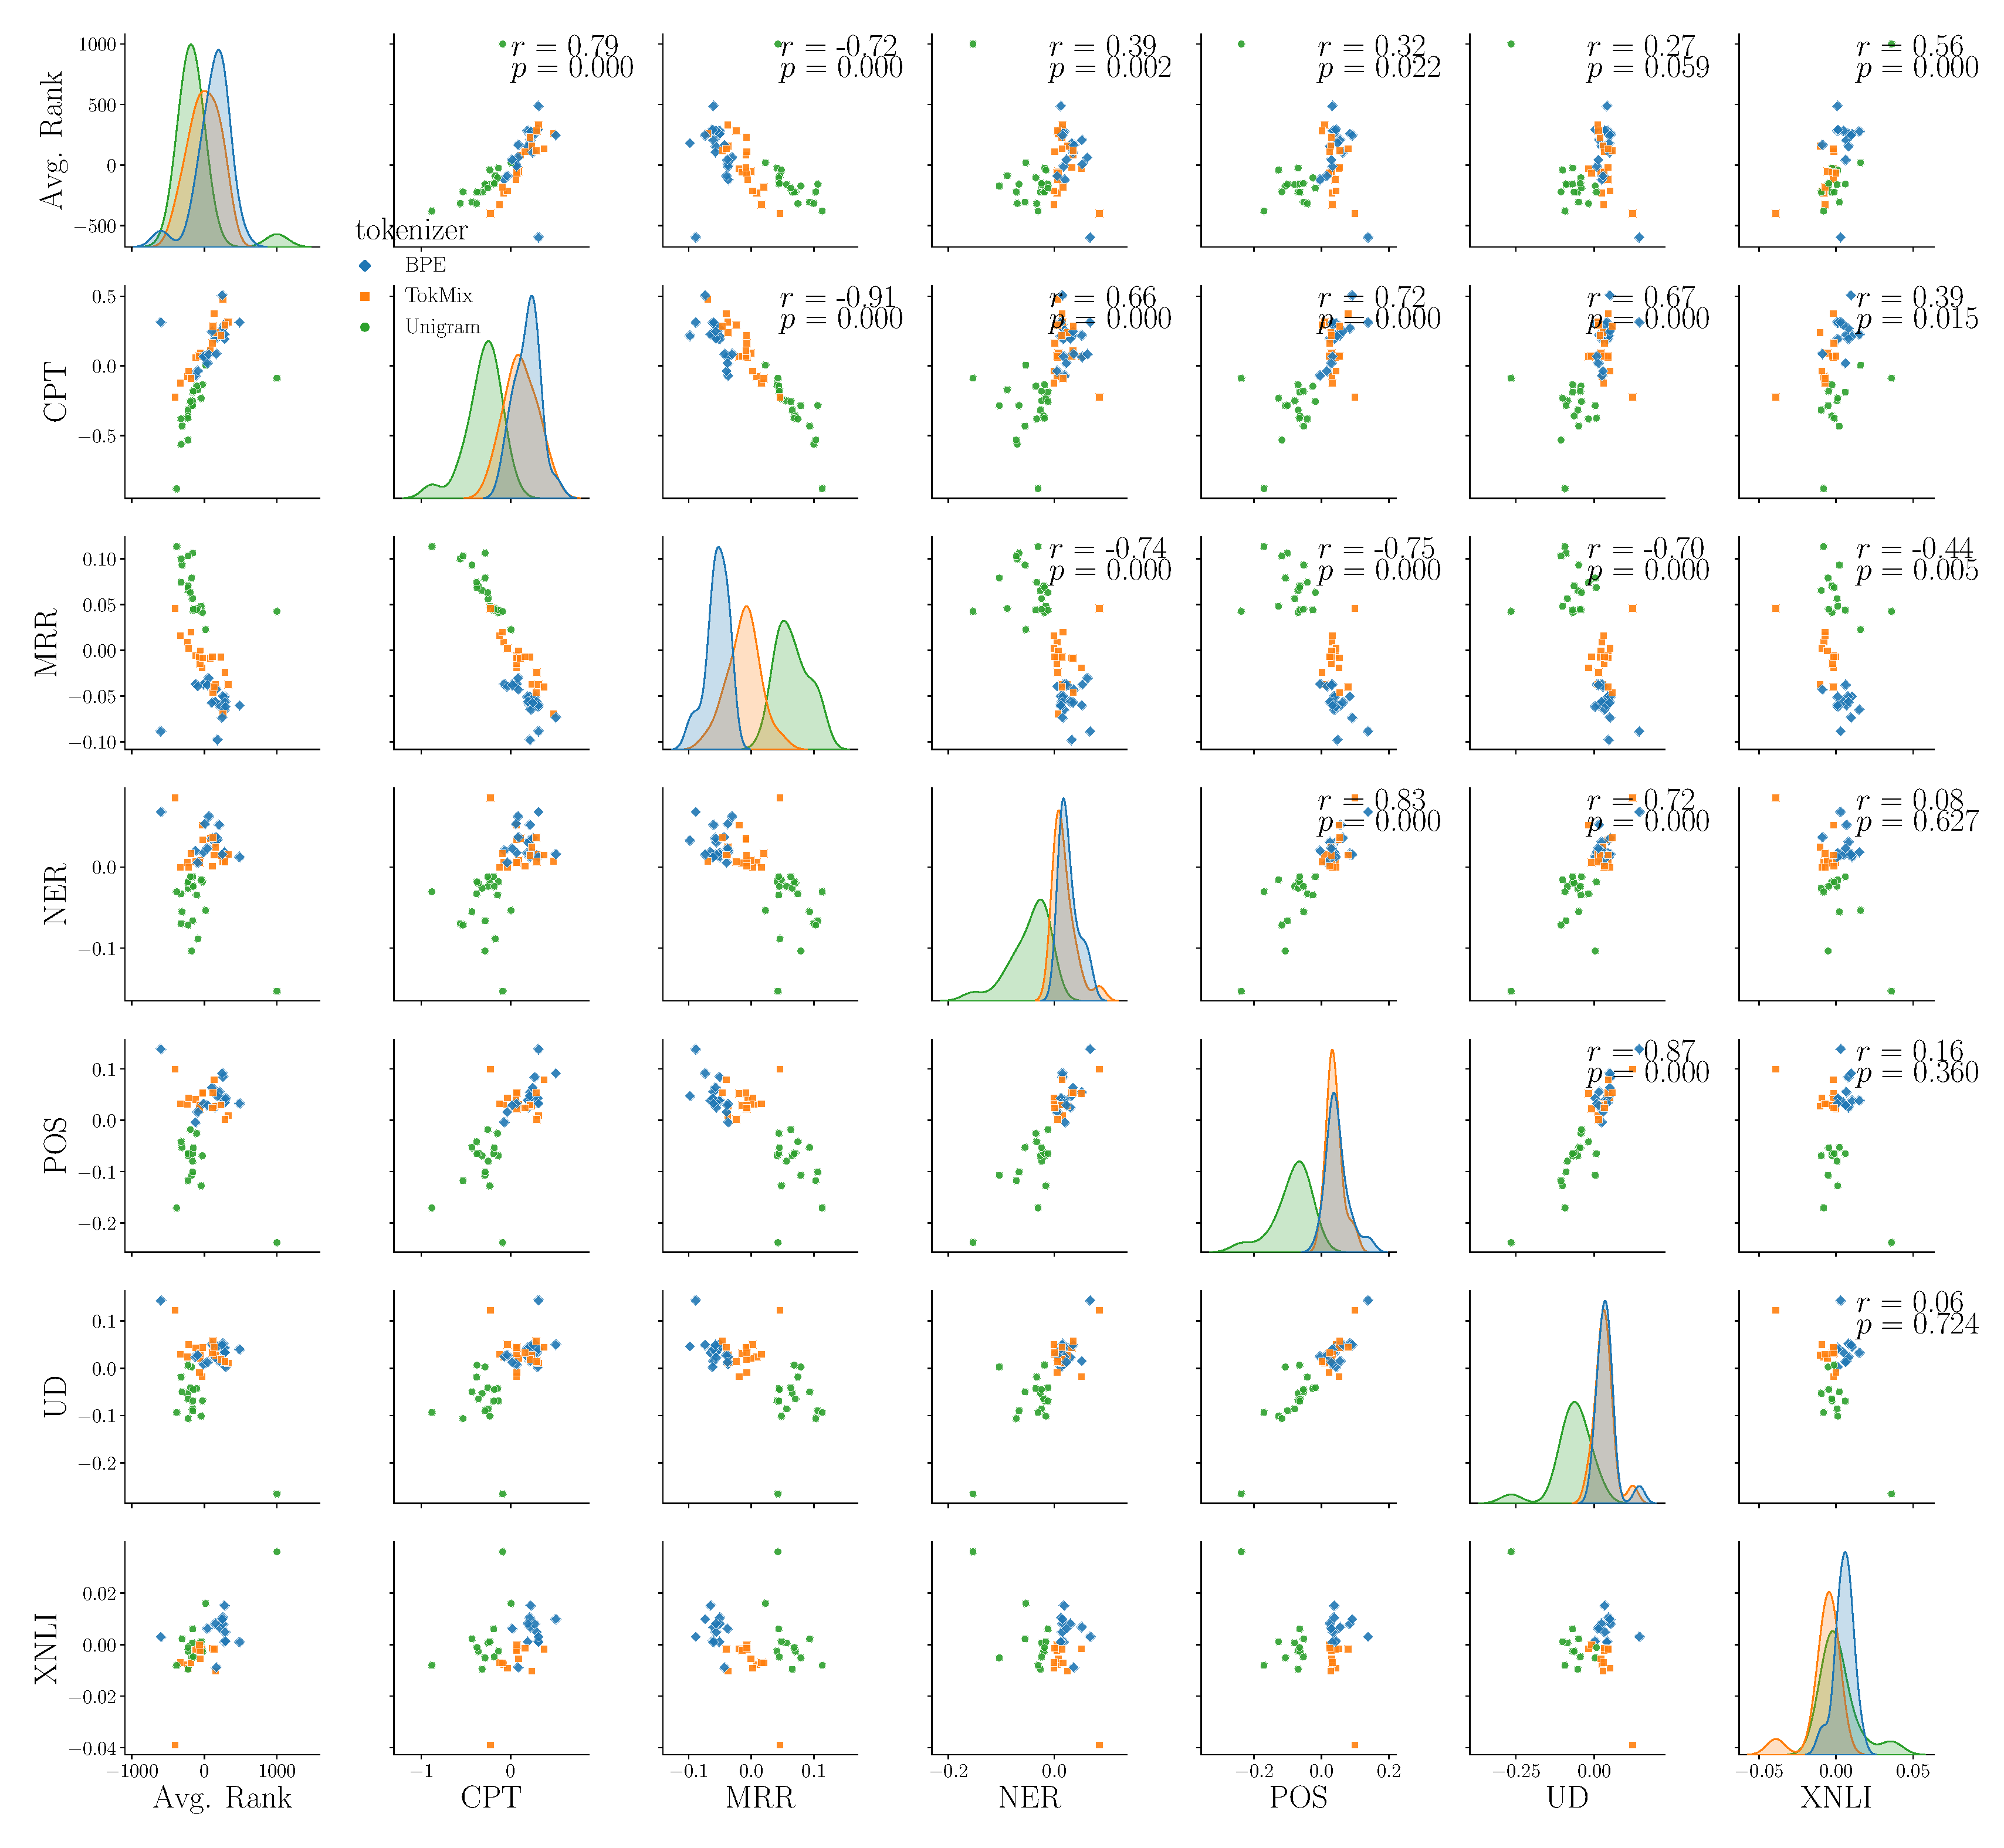
\includegraphics[width=\textwidth]{paper/figures/pair_analysis_20L.pdf}
    \caption{We compare the tokenizer metrics against the contextualized representation quality. For each tokenizer we pretrain a masked language model, freeze it and train a linear probe for each task and each of the available languages. We observe high spearman correlation between CPT and the word-level tasks (NER, POS, UD) and high correlation between AR and the sentence-level task XNLI. This suggests that our vocabulary allocation metrics are good indicators of the tokenizers quality and higher vocabulary allocation leads to better downstream performance. Each data point corresponds to an average result over three seeds of probe training and evaluating on one of the languages. The results for each language are centered around the mean to account for the differences between languages.}
    \label{fig:pair_analysis_20L}
\end{figure}

\begin{figure}[H]
    \centering
    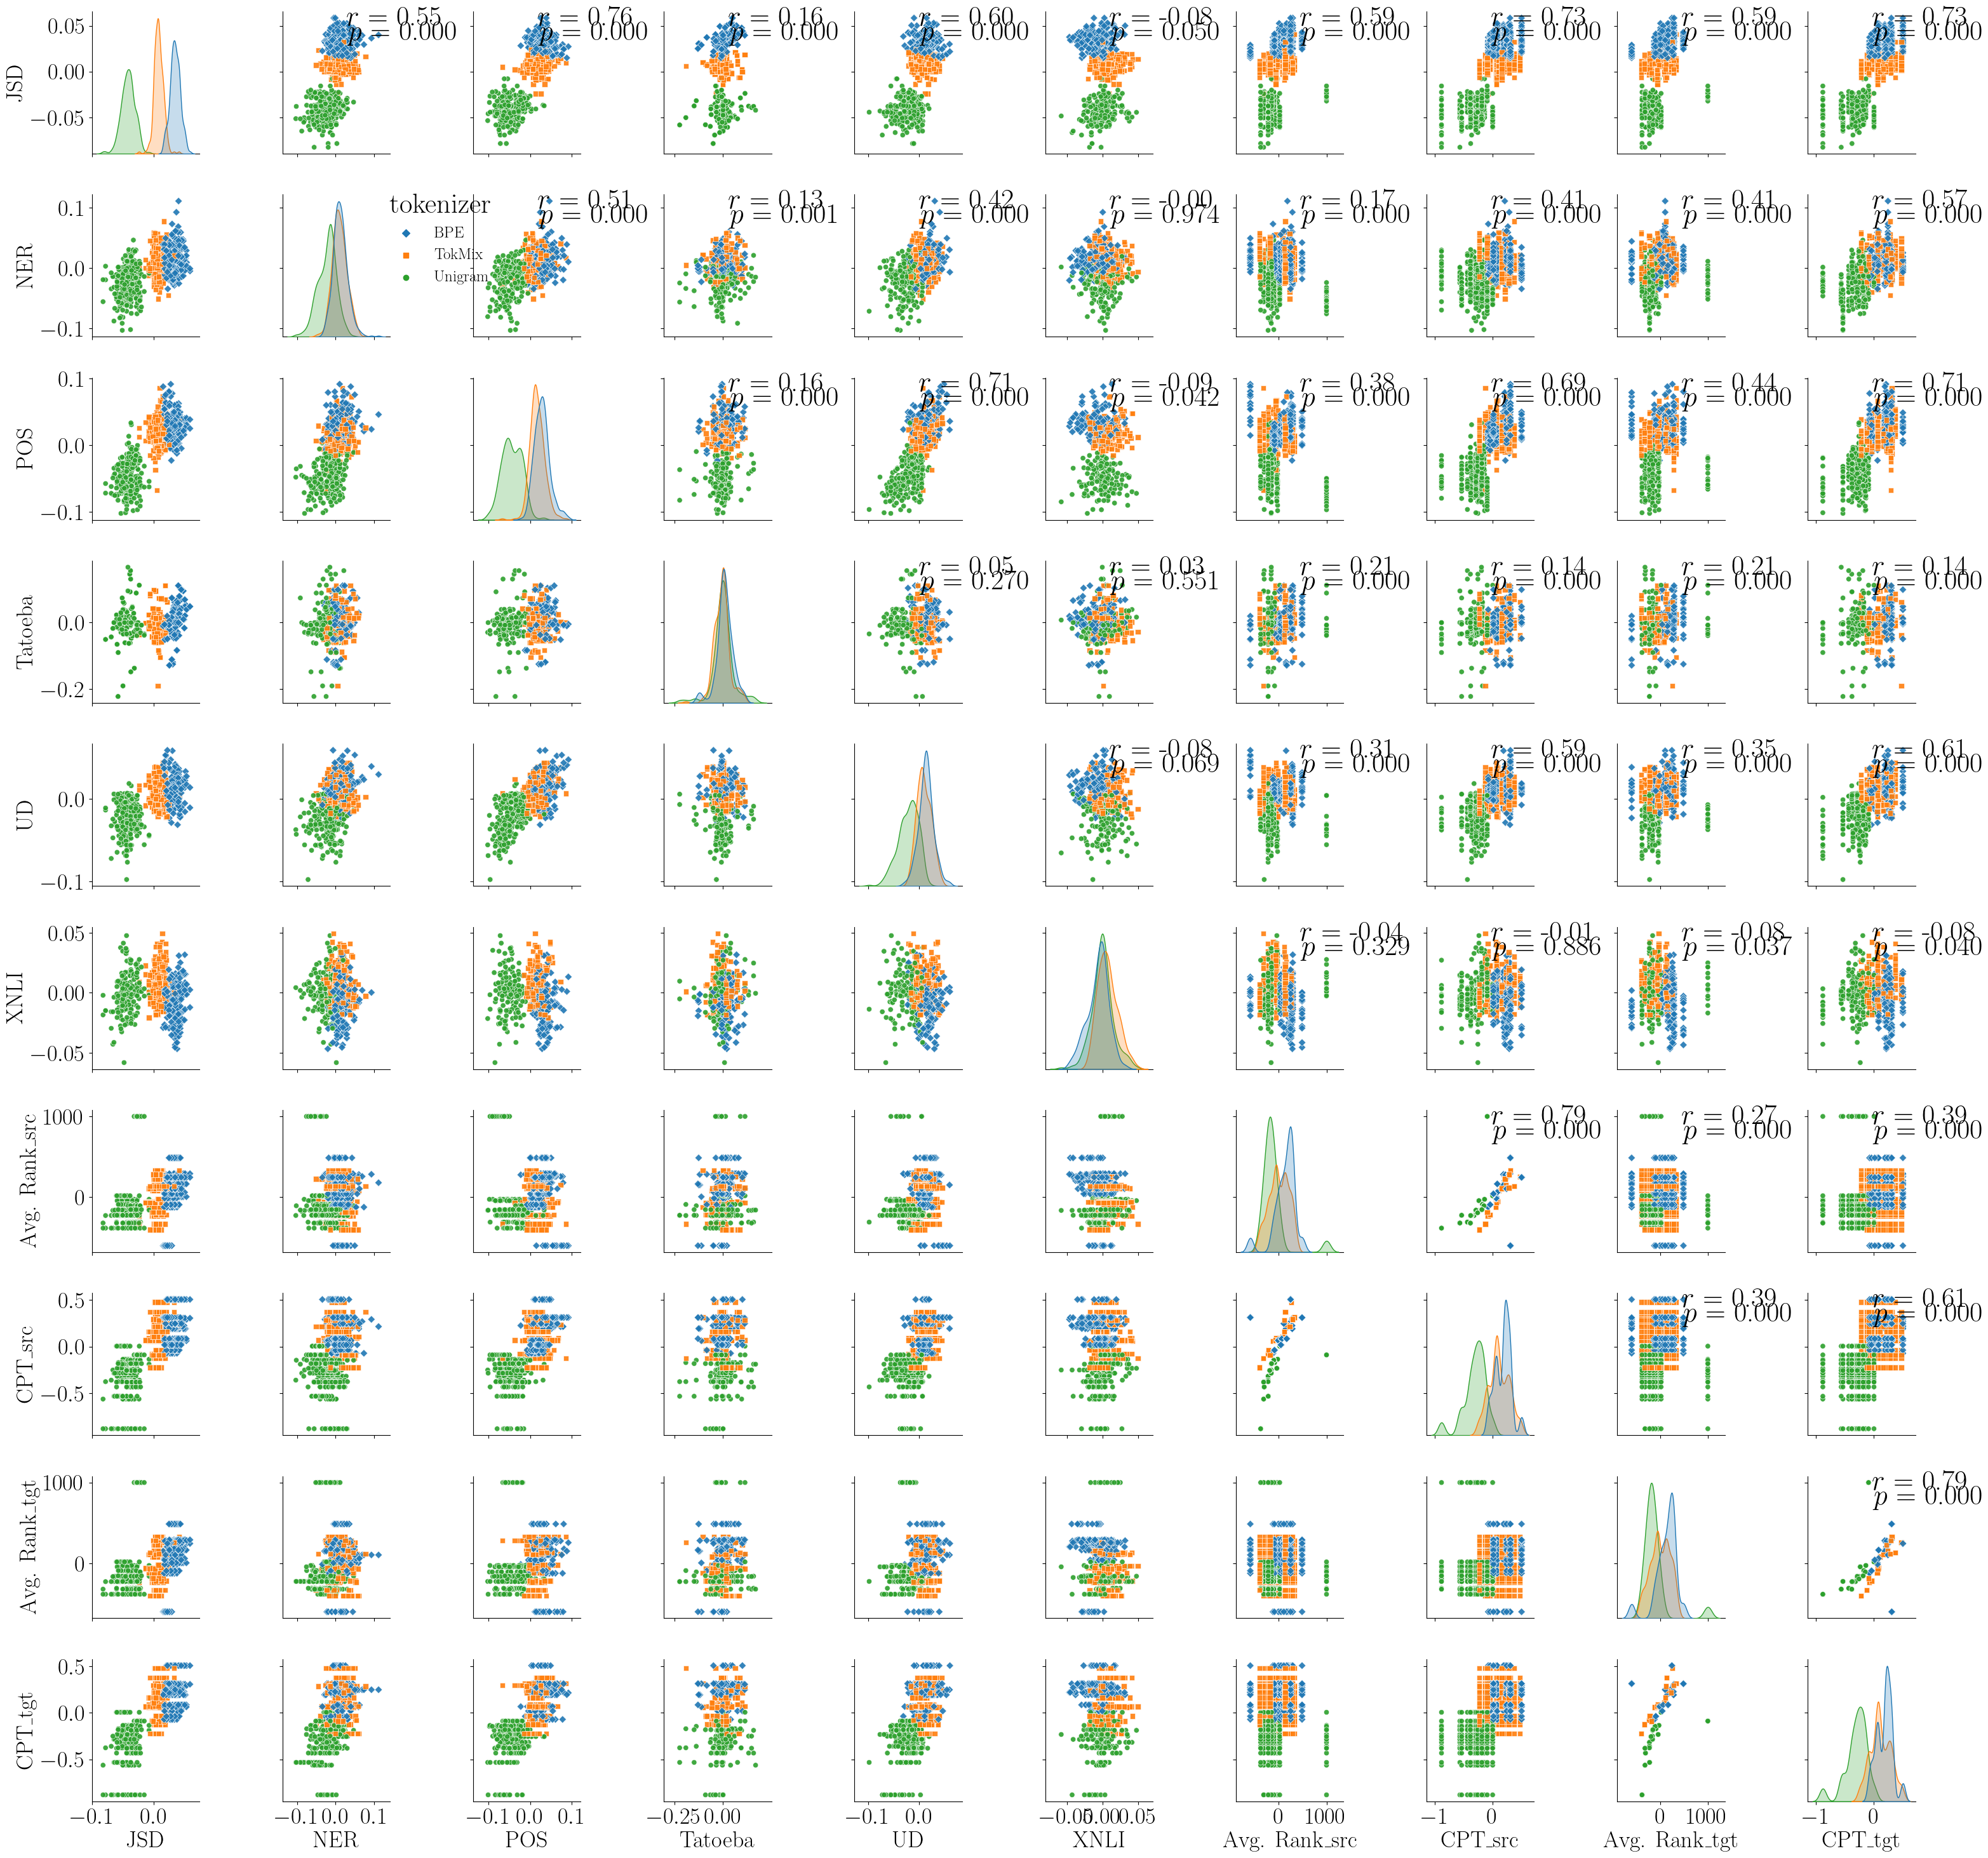
\includegraphics[width=\textwidth]{img/temp/X_pair_analysis_20L.png}
    \caption{We compare the tokenizer metrics against the cross-lingual performance of the models. For each tokenizer we pretrain a masked language model, freeze it and train a linear probe on each of the available languages. Then we evaluate the models on all languages the probe has \textbf{not} been trained on, assessing the cross-lingual properties of the model. Here we observe high correlation between JSD and the word-level tasks, especially the POS and UD. This suggests that less overlap (higher divergence) between the vocabularies of the languages leads to better cross-lingual performance for the word-level tasks.
    \xxx{remove the ar and cpt metrics?}} \xxx{For XNLI, we see low correlation with a marginal p-value.}
    \label{fig:X_pair_analysis_20L}
\end{figure}

\begin{table}
\centering

\begin{tabular}{lccc}
\toprule
 & \multicolumn{2}{c}{\bf{V. Allocation}} & \bf{MLM} \\
 & (AR) &  (CPT)  &  (MRR) \\
\midrule
CPT    &    \bf{0.790} &     - &  - \\
MRR    &  \bf{-0.723} &  \bf{-0.913} &  - \\
NER    &   \bf{0.394} &   \bf{0.657} &  \bf{-0.745} \\
POS    &     0.320 &   \bf{0.724} &  \bf{-0.754} \\
Dep l. &     0.266 &   \bf{0.675} &  \bf{-0.695} \\
NLI   &    \bf{0.56} &    0.388 &  \bf{-0.437} \\ 
\bottomrule
\end{tabular}
\caption{Spearman correlations between centered in-language task results and tokenizer measures. Statistically significant correlations ($p<0.01$) are bolded. Computed for 20 languages.}
\label{tab:corr_in_lang_20l}
\end{table}

\begin{figure}[H]
    \centering
    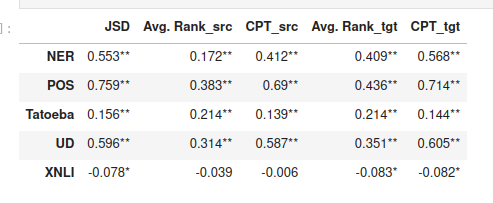
\includegraphics[width=\textwidth]{img/temp/corr_x_lang_20l.png}
    \caption{Correlations between task cross-lingual transfer results and tokenization measures."Stars denote statistical significance: (* coresponeds to $p<0.05$ and ** to $p<0.01$).\xxx{remove the ar and cpt metrics? Merge with the previous correlation table?}}
    \label{fig:corr_x_lang_20l}
\end{figure}

% ---------

\section{The choices that influence the tokenizers quality}

\subsection{Implementation}
\label{sec:implementation}

\begin{table}
\caption{In this table, we compare the Huggingface and Sentencepiece implementations of the Unigram and BPE algorithms. As shown, the Huggingface Unigram tokenizer is a clear outlier in terms of all metrics. We can see that this is a problem in the implementation as the corresponding Sentencepiece \textit{unigram\_alpha0.3} scores much higher. As we will explore in \ref{tab:coverage_influence}, the different alphabet size does not influence the metrics enough to explain the difference. \xxx{here I can add an experiment with the same alphabet size, to be able to skip the reference} Interestingly, we found that the BPE implementation (\textit{huggingface\_bpe\_alpha0.25}) is better in Huggingface than in Sentencepiece (\textit{bpe\_alpha0.25}).}
\label{tab:hugg_vs_sentpiece}
\begin{tabular}{lrrrrr}
\toprule
Tokenizer & Alphabet & \# UNKs & CPT & AR & JSD \\
\midrule
huggingface\_bpe\_alpha0.25 & 1000 & 14040.1 & 3.713 & 1253.7 & 0.783 \\
unigram\_alpha0.3 & 2666 & 923.5 & 3.702 & 1190.7 & 0.768 \\
bpe\_alpha0.25 & 1215 & 7235.6 & 3.666 & 1212.9 & 0.774 \\
huggingface\_unigram\_alpha0.25 & 12616 & 4.5 & 3.204 & 1010.5 & 0.745 \\
\bottomrule
\end{tabular}
\end{table}


As shown in the previous \autoref{sec:influence_of_metrics}, we observe that the Huggingface Unigram tokenizer leads to significantly worse metrics than the other tokenizers. We investigate this difference by turning to the original Sentencepiece implementation of the algorithm and running a comparable experiment with the different library. For comparison, we also train a comparable BPE tokenizer using the Sentencepiece. 

The results are presented in \autoref{tab:hugg_vs_sentpiece}. We see that the implementation has an effect on the tokenization and that the Sentencepiece Unigram tokenizers performs on par with the Huggingface BPE tokenizer. For this reason, we use the Sentencepiece implementation for the rest of the experiments.

\subsection{Data size}
\label{sec:data_size}

\begin{table}
\centering
\caption{We measure how much data is generally needed for the tokenizer training. We train handful of Sentencepiece Unigram tokenizers on different amounts of balanced multilingual data. We observe that after 100k-1M lines per language, the tokenizers converge to similar vocabulary allocation and overlap scores. The significance of this experiment is that we find out experimentally how much data is needed for the tokenizer training and we can use this information to make sure that we provide enough data for each language for the further experiments.}
\label{tab:data_size_influence}
\begin{tabular}{rrrrrr}
\toprule
 Lines per language &  Alphabet size &  Number of UNKs &      CPT &          AR &      JSD \\
\midrule
               1000 &           3598 &          520.35 & 3.301636 &  958.414048 & 0.765687 \\
              10000 &           4725 &          117.75 & 3.597563 & 1089.112498 & 0.765236 \\
             100000 &           5041 &           65.55 & 3.695797 & 1192.201089 & 0.767133 \\
            1000000 &           5079 &           62.60 & 3.702038 & 1204.659073 & 0.767357 \\
            1500000 &           5176 &           55.90 & 3.705119 & 1210.664835 & 0.767348 \\
            2000000 &           5180 &           56.35 & 3.705109 & 1212.489940 & 0.767327 \\
\bottomrule
\end{tabular}
\end{table}


We are interested in how much data is needed for the tokenizer training. For this experiment, we sample the same number of lines (1e3, 1e4, 1e5, 1e6, 1.5e6, 2e6 per language) for each language from the CC100 corpus. Then we train the Sentencepiece Unigram tokenizers on different amounts of data and compare the results in \autoref{tab:data_size_influence}. We see that the metrics improve with the amount of data, but the improvement is not substantial after 100k-1M lines per language. We use these results as a rule of thumb for the rest of the experiments and where possible, we use at least 100k but preferrably 1M lines per language for the rest of the experiments.

\subsection{Character coverage}
\label{sec:character_coverage}

\begin{table}
\caption{We check the tradeoff of including a large alphabet size. We train Sentencepiece Unigram tokenizers with a different target character coverage and observe the resulting alphabet size, number of UNKs and tokenizer metrics. We observe that the alphabet size grows with the coverage and the number of UNKs decreases, as expected. We observe that at both extremes of the character coverage parameter, the vocabulary allocation decreases. The results indicate that the alphabet size between 1000 and 5000 provides a good tradeoff between the number of UNKs and the allocation metrics, while including all characters in the alphabet does not come with a significant decrease in the allocation metrics (-0.05 CPT).}
\label{tab:coverage_influence}
\begin{tabular}{lrrrrr}
\toprule
Coverage & Alphabet & \# UNKs & CPT & AR & JSD \\
\midrule
98.0\% & 539 & 17386.5 & 3.631 & 1115.3 & 0.749 \\
99.5\% & 1136 & 7786.9 & 3.702 & 1173.1 & 0.765 \\
99.95\% & 2678 & 910.6 & 3.705 & 1196.7 & 0.768 \\
99.995\% & 4813 & 83.0 & 3.695 & 1188.7 & 0.769 \\
99.9995\% & 8226 & 10.2 & 3.678 & 1164.2 & 0.769 \\
100.0\% & 13658 & 1.9 & 3.650 & 1124.1 & 0.768 \\
\bottomrule
\end{tabular}
\end{table}


Because we observe the large difference in the alphabet size between Huggingface tokenizers (implied by the use of the default trainer settings of the library), we investigate the influence of this parameter on our tokenizer metrics. We train the Sentencepiece Unigram tokenizers with different character coverage (98\%, 99.5\%, 99.95\%, 99.995\%, 99.9995\%, 99.99995\% and 100.0\%) on balanced data sampled from CC100 with $\alpha=0.0$. and compare the results in \autoref{tab:coverage_influence}. The character coverage parameter determines, how many distinct Unicode characters are included in the vocabulary of the tokenizer. As expected, we see that there is a direct relationship between the character coverage, alphabet size and the number of unknown tokens in the validation set. We also see that our metrics are not largely affected by the alphabet size, as the alphabet accounts for at most 10\% of the whole vocabulary size 120\,000. The lowest vocabulary allocation metrics are on the extremes of the character coverage, where the alphabet size is either very small or very large. We assume that the small alphabet size leads to a large number of unknown tokens and the tokenizer is forced to segment words containing characters outside of the alphabet, as these unknown tokens might even be characters with diacritics. In the range of 1000-5000 alphabet size, we see that the metrics are not largely affected by the alphabet size. On the other extreme, the large alphabet size starts to take up a large portion of the vocabulary and the tokenizer might not have enough capacity to learn longer tokens. For later experiments, we use the Sentencepiece default character coverage of 99.95\%. When comparing tokenizers with different alphabet sizes, we are aware of the fact that the metrics might be affected by the alphabet size and we take this into account when interpreting the results.

\section{Tokenizer training with data imbalance}

\begin{table}
\caption{We train five Sentencepiece Unigram tokenizers on increasingly imbalanced multilingual dataset. We see that the macro averaged metrics decrease with the increasing imbalance, suggesting that on average, the tokenizer represents the languages less well.}
\label{tab:data_balance_metrics}
\begin{tabular}{lrrrrr}
\toprule
Tokenizer & Alphabet & \# UNKs & CPT & AR & JSD \\
\midrule
Unigram $\alpha$=0.0 & 2975 & 617.1 & 3.712 & 1212.9 & 0.767 \\
Unigram $\alpha$=0.3 & 2666 & 923.5 & 3.702 & 1190.7 & 0.768 \\
Unigram $\alpha$=0.5 & 2859 & 729.0 & 3.618 & 1143.8 & 0.769 \\
Unigram $\alpha$=0.7 & 2733 & 883.2 & 3.556 & 1107.1 & 0.770 \\
Unigram $\alpha$=1.0 & 2476 & 1286.3 & 3.442 & 1041.8 & 0.772 \\
\bottomrule
\end{tabular}
\end{table}


In this section, we present the tokenizers that become the baselines for comparing the related works we replicate. Our experiments with the data imbalance follow the original tokenizer training recipe from XLM-R and mBERT. The method is training the tokenizers on a corpus created by combining monolingual data in different proportions. On one extreme we have the $\alpha=1.0$, where all data available for each language is combined. On the other we have $\alpha=0.0$, where the data is sampled per-line from each language with the same probability. 

The contribution of our method is investigating how the language imbalance affects each language individually. Moreover, we investigate how the other proposed methods relate to all settings of $\alpha$, not only the most unbalanced settings of $\alpha=0.5 \textrm{ or } 0.7$.

For the data balancing experiment, we train 5 tokenizers on an increasingly imbalanced corpus with $\alpha = 0.0, 0.3, 0.5, 0.7, 1.0$ using the CC100 with 20 languages. For $\alpha = 0.0, 0.3, 0.5, 0.7$ we make sure to sample at least 100k lines per language as we have found this to be important in \autoref{sec:data_size}. We note that the data imbalance for $\alpha=1.0$ is so large, we needed to settle for 30k-70k training lines for the five least resourceful languages (ka, ur, te, mr, sw) because of memory constrants. We use the Sentencepiece Unigram tokenizer with the default settings. Specifically we use the default character coverage 99.95\%. We evaluate the tokenizers on a balanced validation set sampled from holdout portion of the CC100 corpus. 

The overall results with metrics macro averaged over the 20 languages are presented in \autoref{tab:data_balance_metrics}. The results demonstrate a clear disparity in the performance of the Sentencepiece Unigram, with training on balanced data leading to higher overall metrics than unbalanced data. The imbalance also affects the alphabet as it is possible to cover 99.95\% of the characters in the training data with smaller alphabet because of overrepresentation of few high-resource languages.

We explore the reason for the decreasing performance of the tokenizers trained on imbalanced data in \autoref{fig:data_balance_vs_allocation_per_lang}. We see that the vocabulary allocation metrics for the high resource languages (en, vi, ru, fr, es, th) are improving with the data imbalance. On the other hand, the low resource languages (ka, ur, te, mr, sw) are disproporionally more affected by the imbalance and their vocabulary allocation metrics are decreasing significantly. This suggests that the marginal benefit of adding more data to the high resource languages is lower than the incurred cost on the quality of tokenization for the low resource languages. We see this tradeoff in the \autoref{tab:data_balance_metrics} as a overall decrease in the average CPT and AR.

\begin{figure}[H]
    \centering
    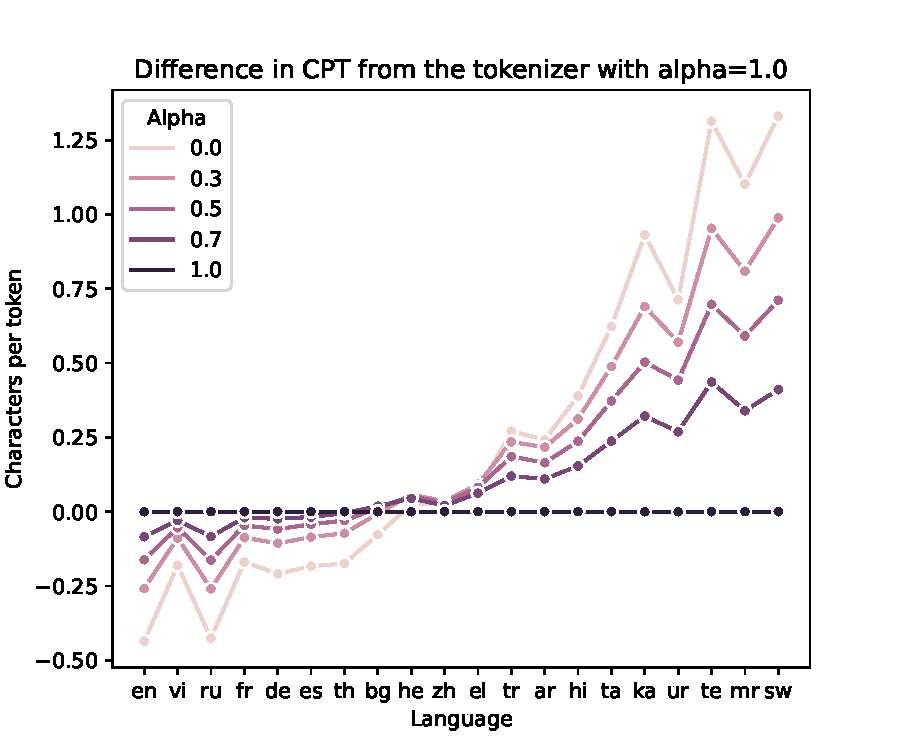
\includegraphics[width=\textwidth]{img/results/cpt_vs_alpha.pdf}
    \caption{We examine the impact of the language imbalance on the Sentencepiece Unigram tokenizer training. We train five tokenizers with an increasing language imbalance controlled by the $\alpha$ parameter. Then we look at the effect on the vocabulary allocation metrics per language. We center the results using the most unbalanced tokenizer with $\alpha=1.0$. As expected, the more balanced tokenizers have higher vocabulary allocation scores for low resource languages and lower scores for high resource languages. Interestingly, the effect varies across languages. For example the vocabulary allocation of high-resource Vietnamese or French is not as affected by the decrease in training data as English or Russian. \xxx{We also observe that the data imbalance negatively affects the low resource languages more than it positively affects the high resource languages. This suggests that the marginal benefit of adding more data to the high resource languages is lower than the incurred cost on the quality of tokenization for the low resource languages. <- is this a good interpretation?}}
    \label{fig:data_balance_vs_allocation_per_lang}
\end{figure}


\section{Comparison of balancing methods}
\subsection{Balancing methods and vocabulary allocation}

\begin{table}
\caption{In this summary table, we present all tokenizers used in this chapter. Along with the Huggingface tokenizers from table \ref{fig:20l_metrics} and Sentencepiece Unigram tokenizers from \ref{fig:data_balance_vs_allocation_per_lang}, we include the tokenizers obtained by replicating the papers \citet{chung_improving_2020,zheng_allocating_2021,liang_xlm-v_2023} in our setting. As we can see, the Huggingface Unigram tokenizer is a clear outlier in terms of all metrics even after taking account the higher alphabet size as explored in \ref{tab:coverage_influence}. Further we can see that the proposed balancing methods are improving over the baselines the authors used (\textit{unigram\_alpha0.5} and \textit{unigram\_alpha0.7}). On the other hand we see that using more balanced data for training the Sentencepiece Unigram (\textit{unigram\_alpha0.0}) does lead to similar overall performance as the replicated methods.
The rows are sorted by the CPT score. \xxx{As we can see that except for the Huggingface tokenizers, the alphabet sizes for all tokenizers stay in the stable range of 1000-5000. This corresponds to a comparable number number of UNKs in the holdout data.
}}
\label{tab:all_tokenizers_metrics}
\begin{tabular}{lrrrrr}
\toprule
Tokenizer & Alphabet & \# UNKs & CPT & AR & JSD \\
\midrule
huggingface\_bpe\_alpha0.25 & 1000 & 14040.1 & 3.713 & 1253.7 & 0.783 \\
unigram\_alpha0.0 & 2975 & 617.1 & 3.712 & 1212.9 & 0.767 \\
Chung\_20clusters & 4123 & 270.3 & 3.702 & 1098.7 & 0.766 \\
unigram\_alpha0.3 & 2666 & 923.5 & 3.702 & 1190.7 & 0.768 \\
TokMix\_alpha0.25 & 2497 & 1203.2 & 3.691 & 1163.4 & 0.773 \\
Chung\_16clusters & 3933 & 387.1 & 3.677 & 1102.2 & 0.767 \\
Liang\_20clusters & 3709 & 341.4 & 3.676 & 1103.2 & 0.765 \\
Zheng\_20langs & 4854 & 245.7 & 3.673 & 1094.5 & 0.765 \\
Liang\_16clusters & 3655 & 416.8 & 3.669 & 1106.2 & 0.767 \\
bpe\_alpha0.25 & 1215 & 7235.6 & 3.666 & 1212.9 & 0.774 \\
unigram\_alpha0.5 & 2859 & 729.0 & 3.618 & 1143.8 & 0.769 \\
Chung\_8clusters & 4870 & 684.4 & 3.575 & 1061.1 & 0.770 \\
unigram\_alpha0.7 & 2733 & 883.2 & 3.556 & 1107.1 & 0.770 \\
Chung\_4clusters & 3253 & 648.6 & 3.546 & 1071.9 & 0.768 \\
Liang\_8clusters & 4283 & 568.2 & 3.544 & 1081.6 & 0.767 \\
Liang\_4clusters & 3698 & 419.2 & 3.512 & 1082.5 & 0.769 \\
unigram\_alpha1.0 & 2476 & 1286.3 & 3.442 & 1041.8 & 0.772 \\
huggingface\_unigram\_alpha0.25 & 12616 & 4.5 & 3.204 & 1010.5 & 0.745 \\
\bottomrule
\end{tabular}
\end{table}


\begin{figure}[H]
    \centering
    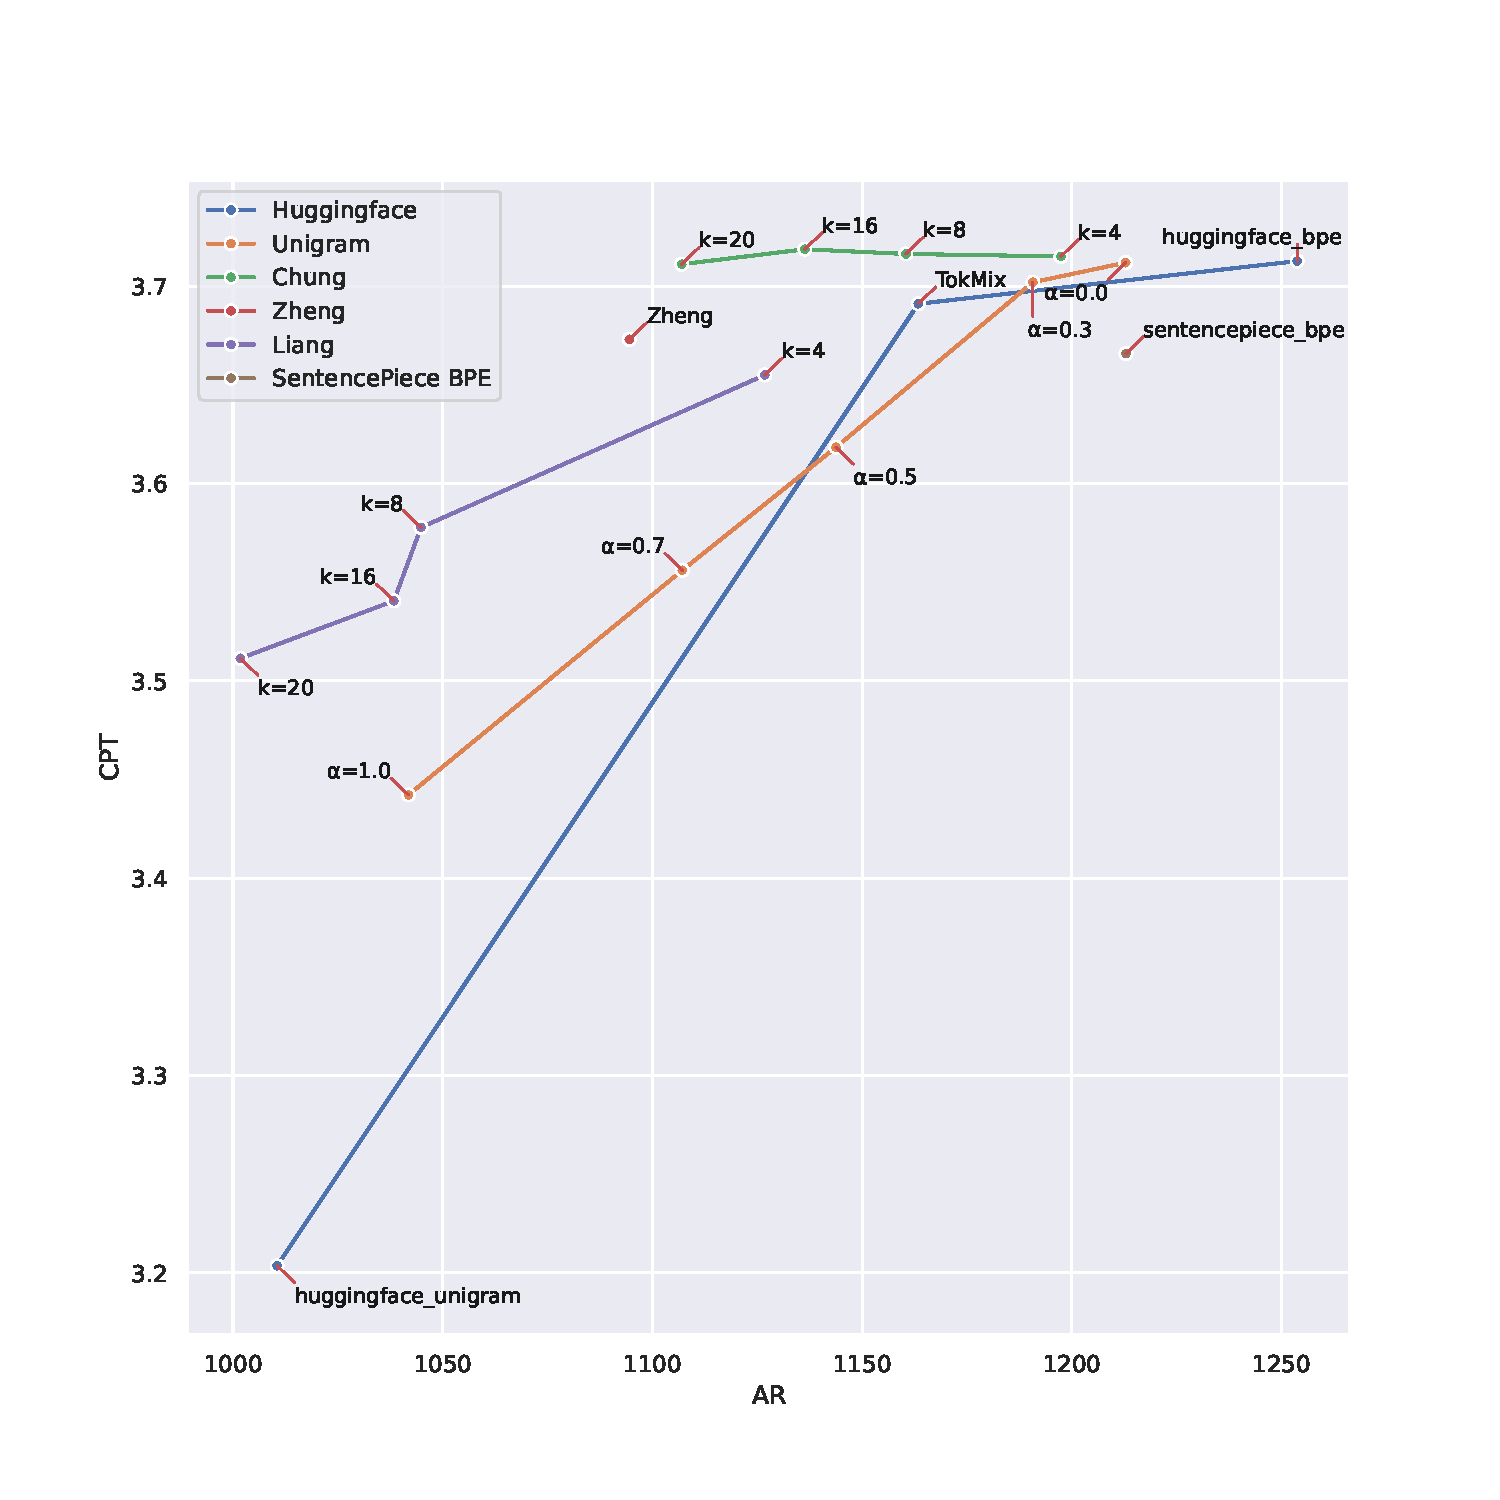
\includegraphics[width=\textwidth]{figures/all_tokenizers_AR_vs_CPT.pdf}
    \caption{We visualize the overall vocabulary allocation metrics for all tokenizers from Table \ref{tab:all_tokenizers_metrics}. We observe that the vocabulary allocation scores are related --- higher AR usually means higher CPT. Nevertheless, we also have tokenizers with low AR and high CPT but never the other way around. Our intuition is that it is not possible to construct a tokenizer with high number of useful tokens which are all very short. We also observe that Huggingface Unigram is a clear outlier, although combination of separate, monolingual Huggingface Unigrams (TokMix) approaches the performance of the Sentencepiece Unigram with the corresponding data imbalance ($\alpha=0.3$). We again see, that the balancing methods, especially Chung and Zheng overperform the unbalanced baselines ($\alpha=0.7$, $\alpha=0.5$) but perform similarly or worse to the simple case of running the Sentencepiece Unigram trainer on a balanced set $\alpha=0.0$.}
    \label{fig:all_tokenizers_AR_vs_CPT}
\end{figure}

\begin{figure}[H]
    \centering
    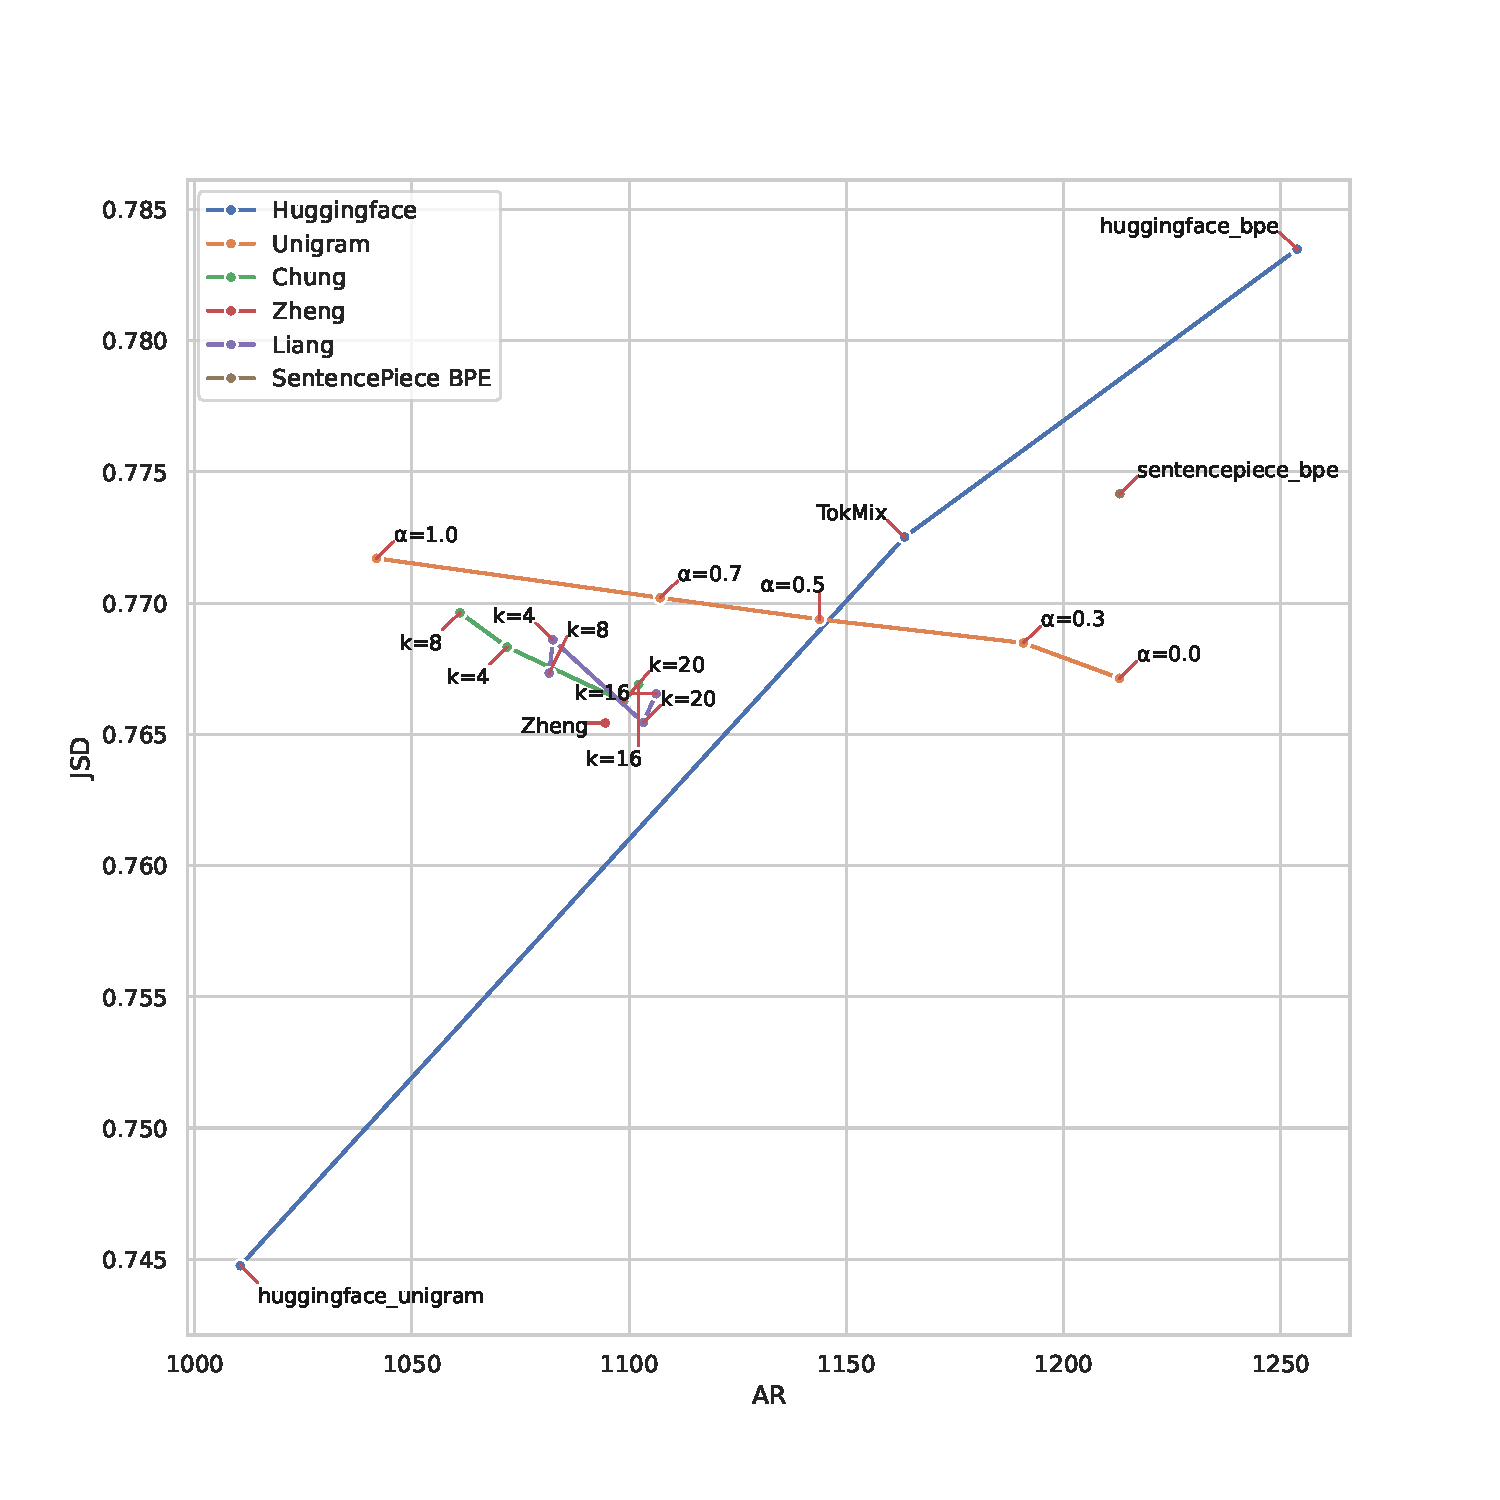
\includegraphics[width=\textwidth]{figures/all_tokenizers_AR_vs_JSD.pdf}
    \caption{We visualize the tokenizers from Table \ref{tab:all_tokenizers_metrics} in terms of Average Rank and Jensen-Shannon Divergence. Here we can see that all methods based on Sentencepiece result in similar overlap independent of the allocation. This is interesting because the replicated balancing methods (Chung, Zheng, Liang) work by splitting the data and training separate tokenizers. Nevertheless, after merging the separate subtokenizers they all seem to end up with similar vocabulary overlaps. The highest vocabulary isolation is surprisingly achieved by the Huggingface BPE tokenizer, which is contrary to the hypothesis stated by \citet{chung_improving_2020,zheng_allocating_2021} that the tokenizers trained on the concatenation of all data tend to select subwords shared across all languages.}
    \label{fig:all_tokenizers_AR_vs_JSD}
\end{figure}

\begin{figure}[H]
    \centering
    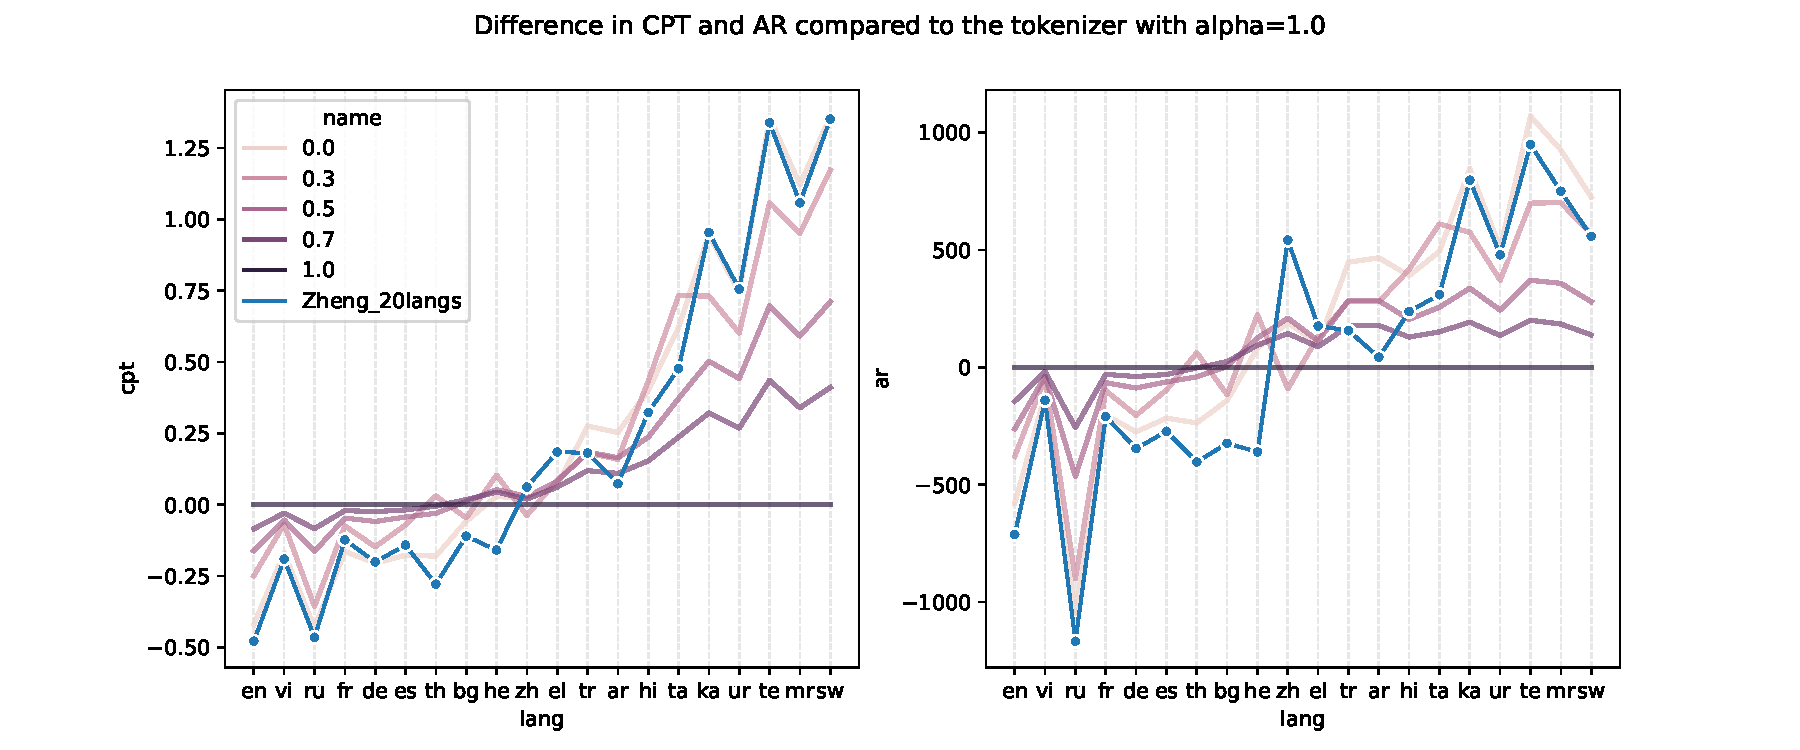
\includegraphics[width=\textwidth]{figures/zheng_vs_alphas.pdf}
    \caption{We zoom into the results of the Zheng method and compare the vocabulary allocation across the individual languages represented by this tokenizer against the backdrop of the vanilla Unigram tokenizers trained with different data imbalances from \ref{fig:data_balance_vs_allocation_per_lang}. We observe a striking similarity between the vocabulary allocation of the Zheng tokenizer and the Unigram tokenizer with $\alpha=0.0$, especially in terms of characters per token. This comes as a large surprise because the Zheng method works by training a separate tokenizer for each language and then merging them together. Despite the different method of obtaining the vocabulary, the resulting tokenizers are very similar across the languages.}
    \label{fig:zheng_vs_alphas}
\end{figure}

\begin{figure}[H]
    \centering
    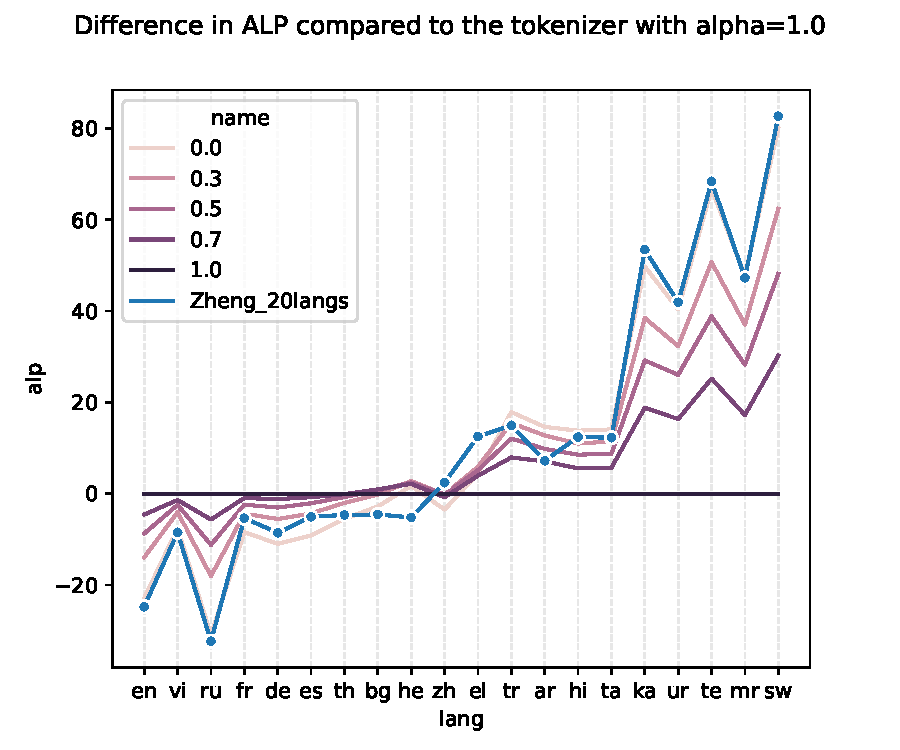
\includegraphics[width=\textwidth]{figures/zheng_vs_alphas_alp.pdf}
    \caption{Intrigued by the similarity between the Zheng tokenizer and the Unigram tokenizer with $\alpha=0.0$ from Figure \ref{fig:zheng_vs_alphas} we also look at the ALP metric which is used for the selection of vocabulary sizes in the Zheng method. Here we see that the greedy optimization of ALP across languages indeed results in a similar vocabulary allocation as the Unigram tokenizer with $\alpha=0.0$.}
    \label{fig:zheng_vs_alphas_alp}
\end{figure}



\begin{figure}[H]
    \centering
    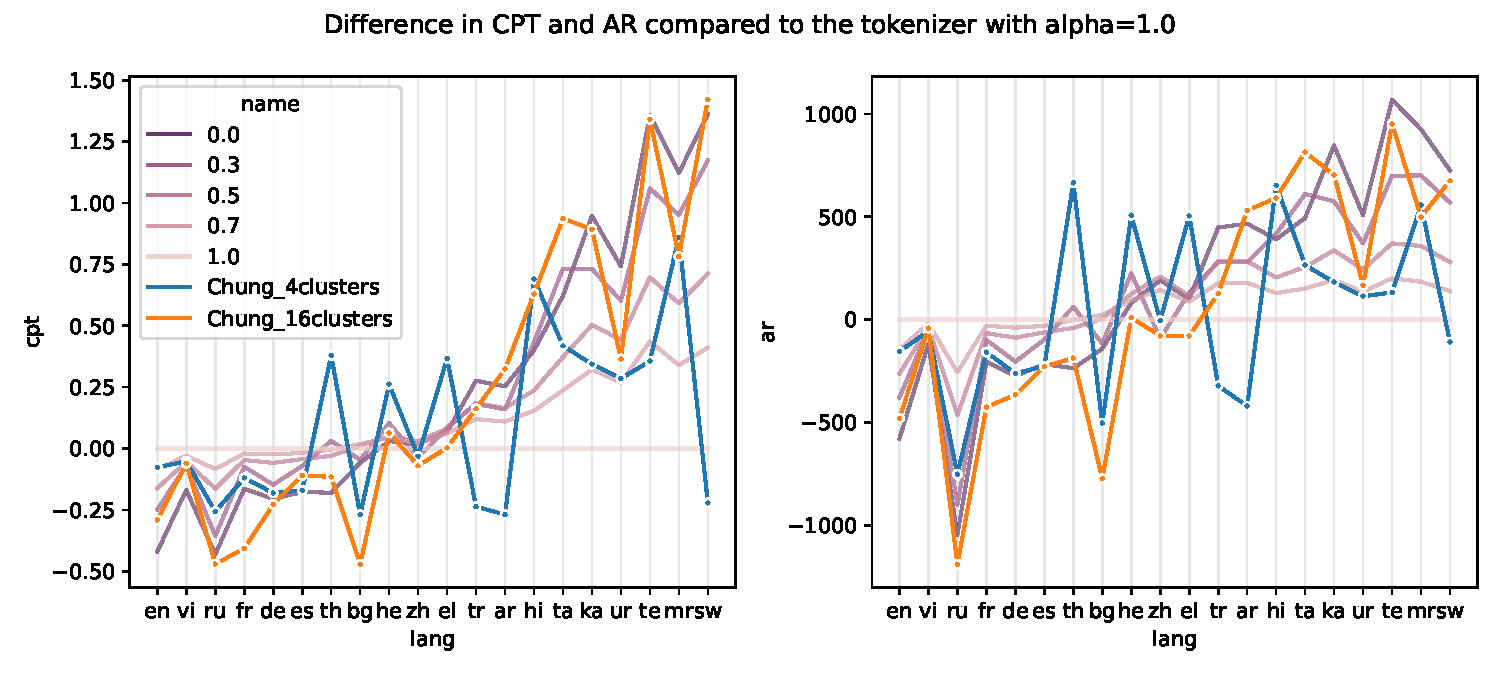
\includegraphics[width=\textwidth]{figures/chung_vs_alphas.pdf}
    \caption{Here we inspect the language-level vocabulary allocation of the Chung method. Similarly to the Zheng method, the Chung method also performs similarly to the Unigram tokenizer with $\alpha=0.0$. Unfortunately, we believe this is an artifact of the choice of our training data for the Chung method. We use a balanced dataset ($\alpha=0.0$) for training the cluster-specific tokenizers. The balance of the data seems to be more important than the clustering step. After merging the cluster-specific tokenizers, the resulting tokenizer is very similar to the Unigram tokenizer with $\alpha=0.0$.}
    \label{fig:chung_vs_alphas}
\end{figure}

\begin{figure}[H]
    \centering
    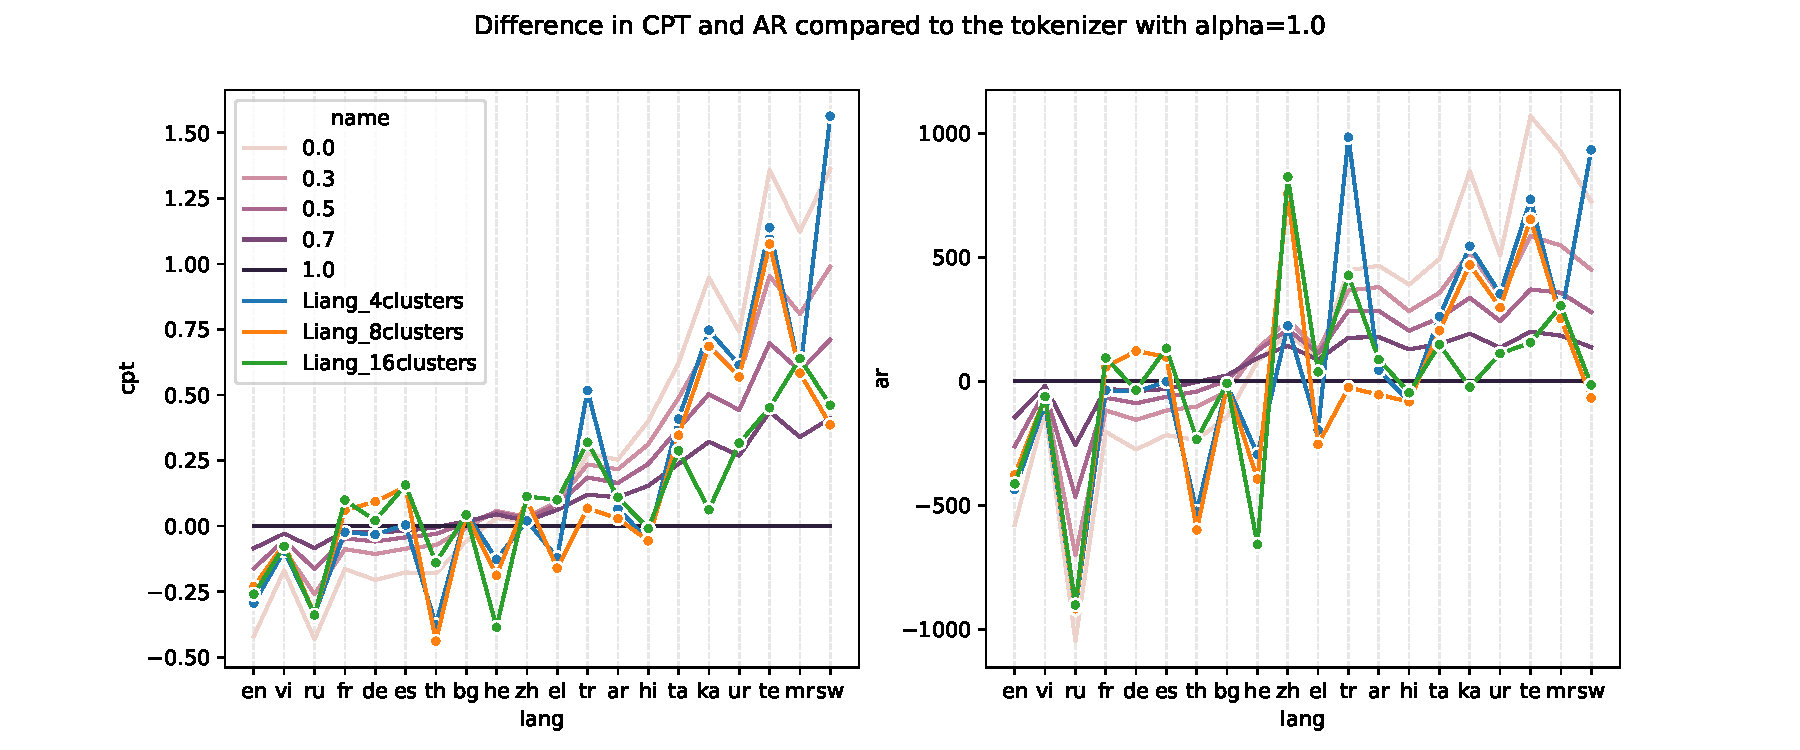
\includegraphics[width=\textwidth]{figures/liang_vs_alphas.pdf}
    \caption{Interestingly, the Liang method seems to yield the most distinct results despite the fact it is trained with balanced data and uses the greedy allocations from the Zheng method. \xxx{TODO: explain why}}
    \label{fig:liang_vs_alphas}
\end{figure}

\subsection{Balancing methods and vocabulary overlap}
\section{Comparison of balancing methods on downstream tasks}


\begin{figure}
    \centering
    \begin{subfigure}{.5\textwidth}
      \centering
      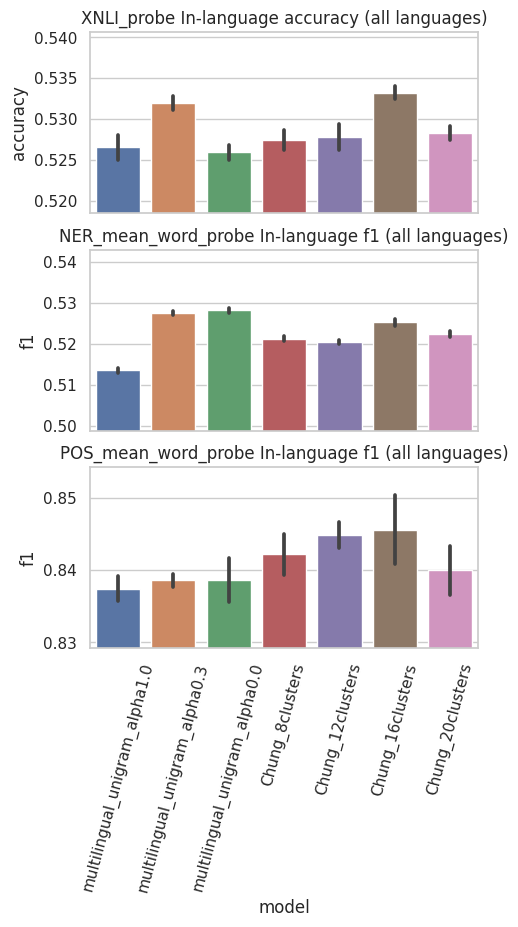
\includegraphics[width=\linewidth]{img/temp/probe_overall_inlanguage.png}
      \caption{In-language results}
      \label{fig:probe_overall_inlanguage}
    \end{subfigure}%
    \begin{subfigure}{.5\textwidth}
      \centering
      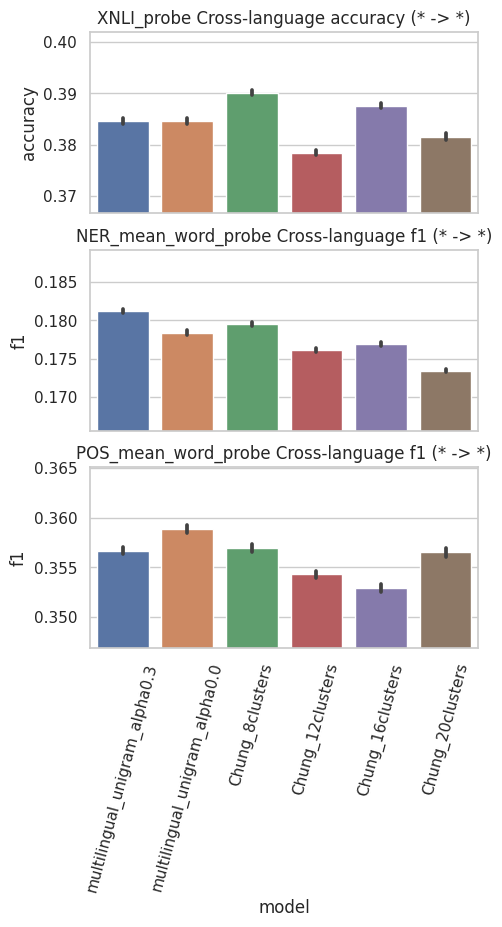
\includegraphics[width=\linewidth]{img/temp/probe_overall_crosslanguage.png}
      \caption{Cross-language results}
      \label{fig:probe_overall_crosslanguage}
    \end{subfigure}
    \caption{We select the best performing balancing method by \citet{chung_improving_2020} from our replications based on our tokenizer metrics and compare it with the vanilla Unigram tokenizers. We choose the unbalanced Unigram tokenizer with $\alpha=1.0$ and then two stronger baselines with $\alpha=0.0$ and $\alpha=0.3$ trained on more balanced data. We then pretrain masked language models that differ only in the tokenizer they use and assess the performance of these models on the downstream tasks using probing. We test two settings --- in-language performance, where the model is trained on each of the available languages and then evaluated on the same language, and cross-language performance, where the model is also trained on each language but evaluated on all \textit{but} the training language. We observe that for word-level tasks all balanced tokenizers (where $\alpha\neq1.0$) perform significantly better than the unbalanced Unigram. Moreover we see that the differences between the individual balancing methods seem to be minimal. For sentence-level NLI, we do not observe any systematic effects as the differences between the runs are quite low (<1\% accuracy).
    The results are a macro average over all the languages (in-language results) or language pairs (cross-language results). For each model and language we do 3 probe training runs with different random seeds. The error bars represent one standard deviation computed with bootstrapping by randomly sampling seeds for each language. Note that even though the probe training is done with three different random seeds, the model pretraining was done only once. The variance between pretraining runs is therefore not measured and the error bars should be interpreted as such.}
    \label{fig:probe_overall}
\end{figure}

% \begin{figure}[H]
%     \centering
%     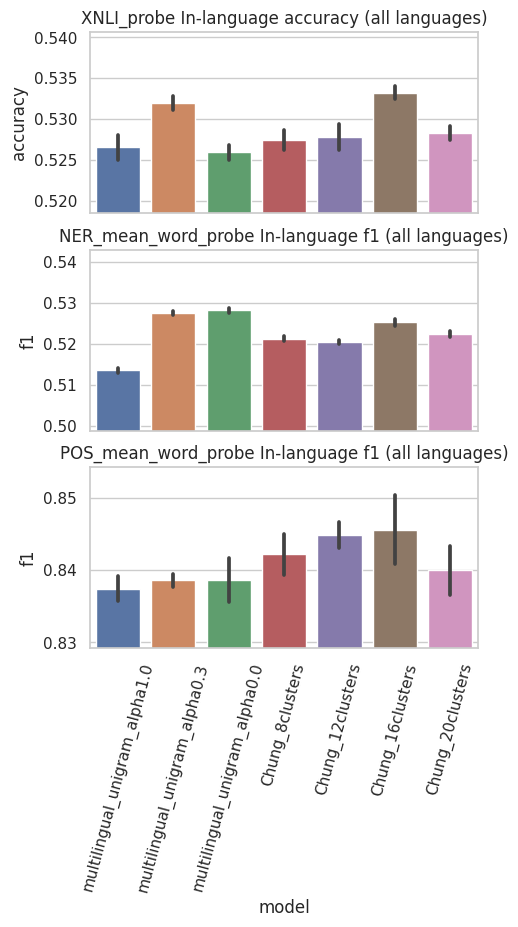
\includegraphics[width=\textwidth]{img/temp/probe_overall_inlanguage.png}
%     \caption{probe overall inlanguage}
%     \label{fig:probe_overall_inlanguage}
% \end{figure}


\begin{figure}[H]
    \centering
    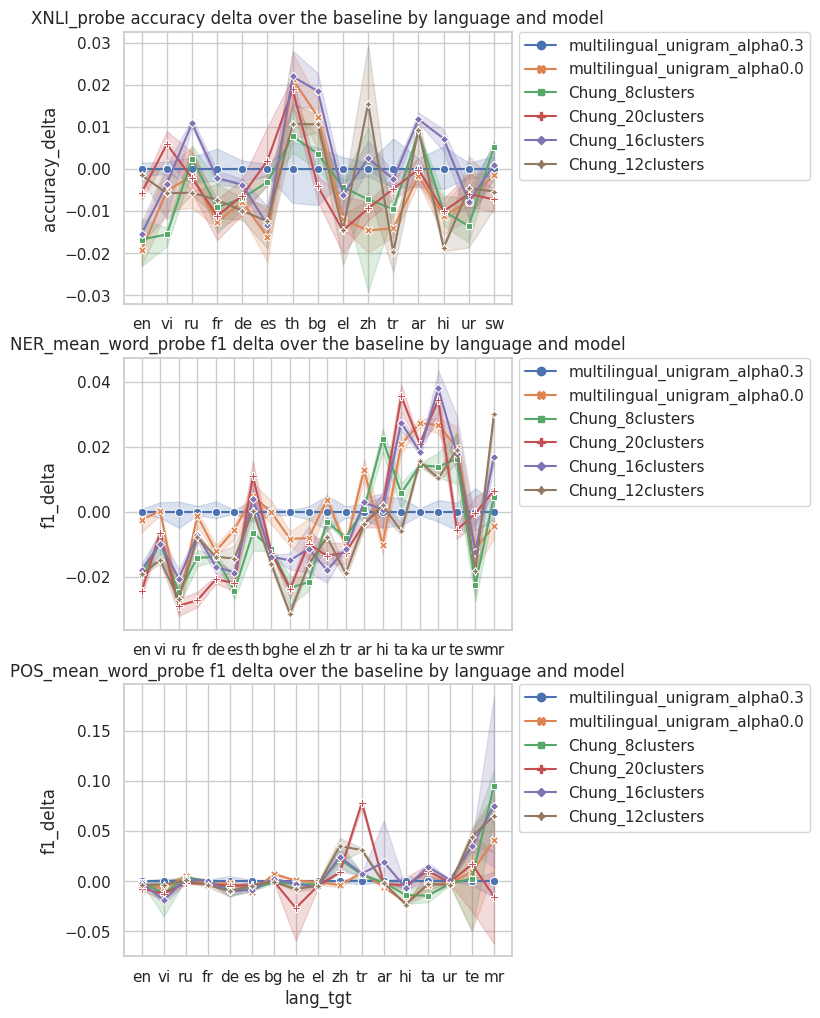
\includegraphics[width=\textwidth]{img/temp/probe_overall_inlanguage_over_baseline.png}
    \caption{We zoom in on the in-language results from Figure \ref{fig:probe_overall_inlanguage} and compare the performance of the balanced tokenizers against the unbalanced Unigram tokenizer with $\alpha=1.0$ over all tested languages for the tasks. In case of the word-level tasks, especially in the case of named entity recognition, we observe a clear trend in line with our tokenizer investigations in \ref{fig:chung_vs_alphas}. The balancing methods improve the language representations for the word-level tasks. For the sentence-level tasks, we do not observe any systematic effects. This might be in part due to the fact that the NLI task does not include 4 of our low-resource languages. The error bands are one standard deviation computed from the three probe training runs with different random seeds.}
    \label{fig:probe_overall_inlanguage_over_baseline}
\end{figure}


\begin{figure}[H]
    \centering
    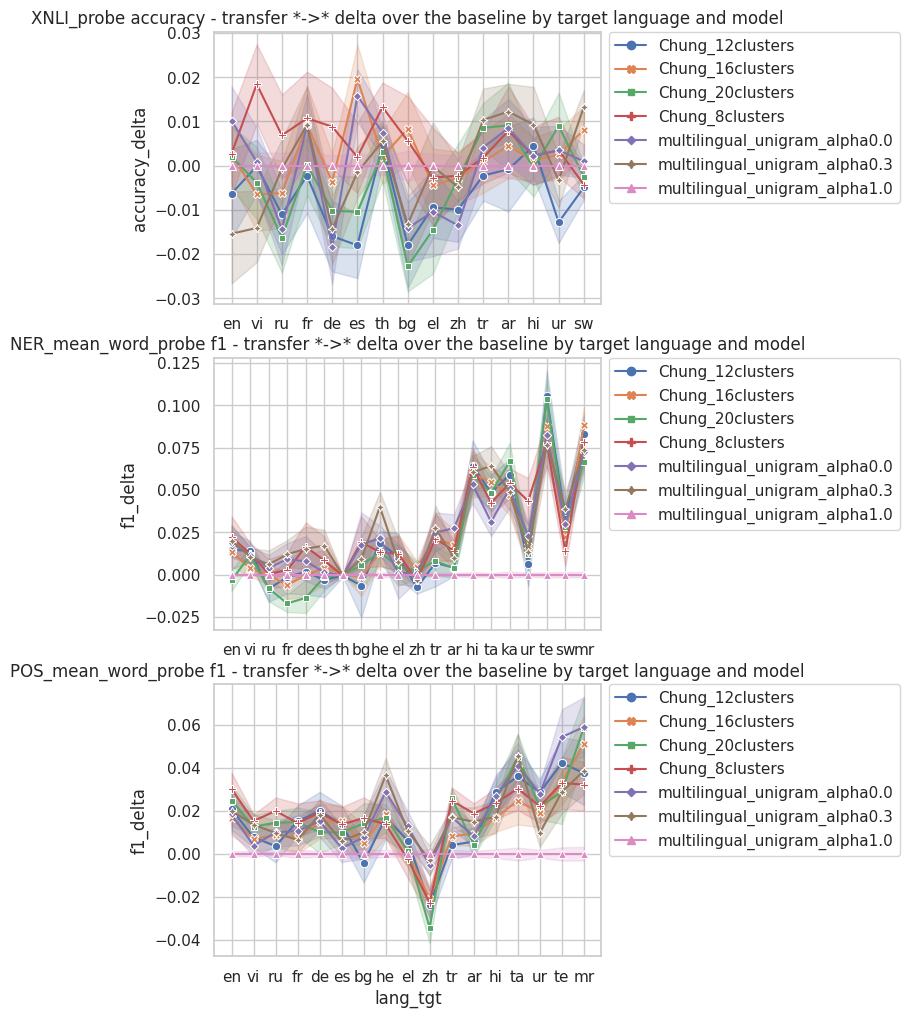
\includegraphics[width=\textwidth]{img/temp/probe_overall_crosslanguage_over_baseline.png}
    \caption{Here we investigate in detail the cross-lingual results from Figure \ref{fig:probe_overall_crosslanguage} with comparison to the unbalanced Unigram tokenizer with $\alpha=1.0$. We observe that word-level task transfers behave in line with the tokenizer investigations in \ref{fig:chung_vs_alphas}. Moreover it seems that both high-resource and low-resource languages benefit from the balancing methods, although the change is most clear at the low-resource side. For the sentence-level tasks, we do not observe any systematic effects.}
    \label{fig:probe_overall_crosslanguage_over_baseline}
\end{figure}



\begin{figure}[H]
    \centering
    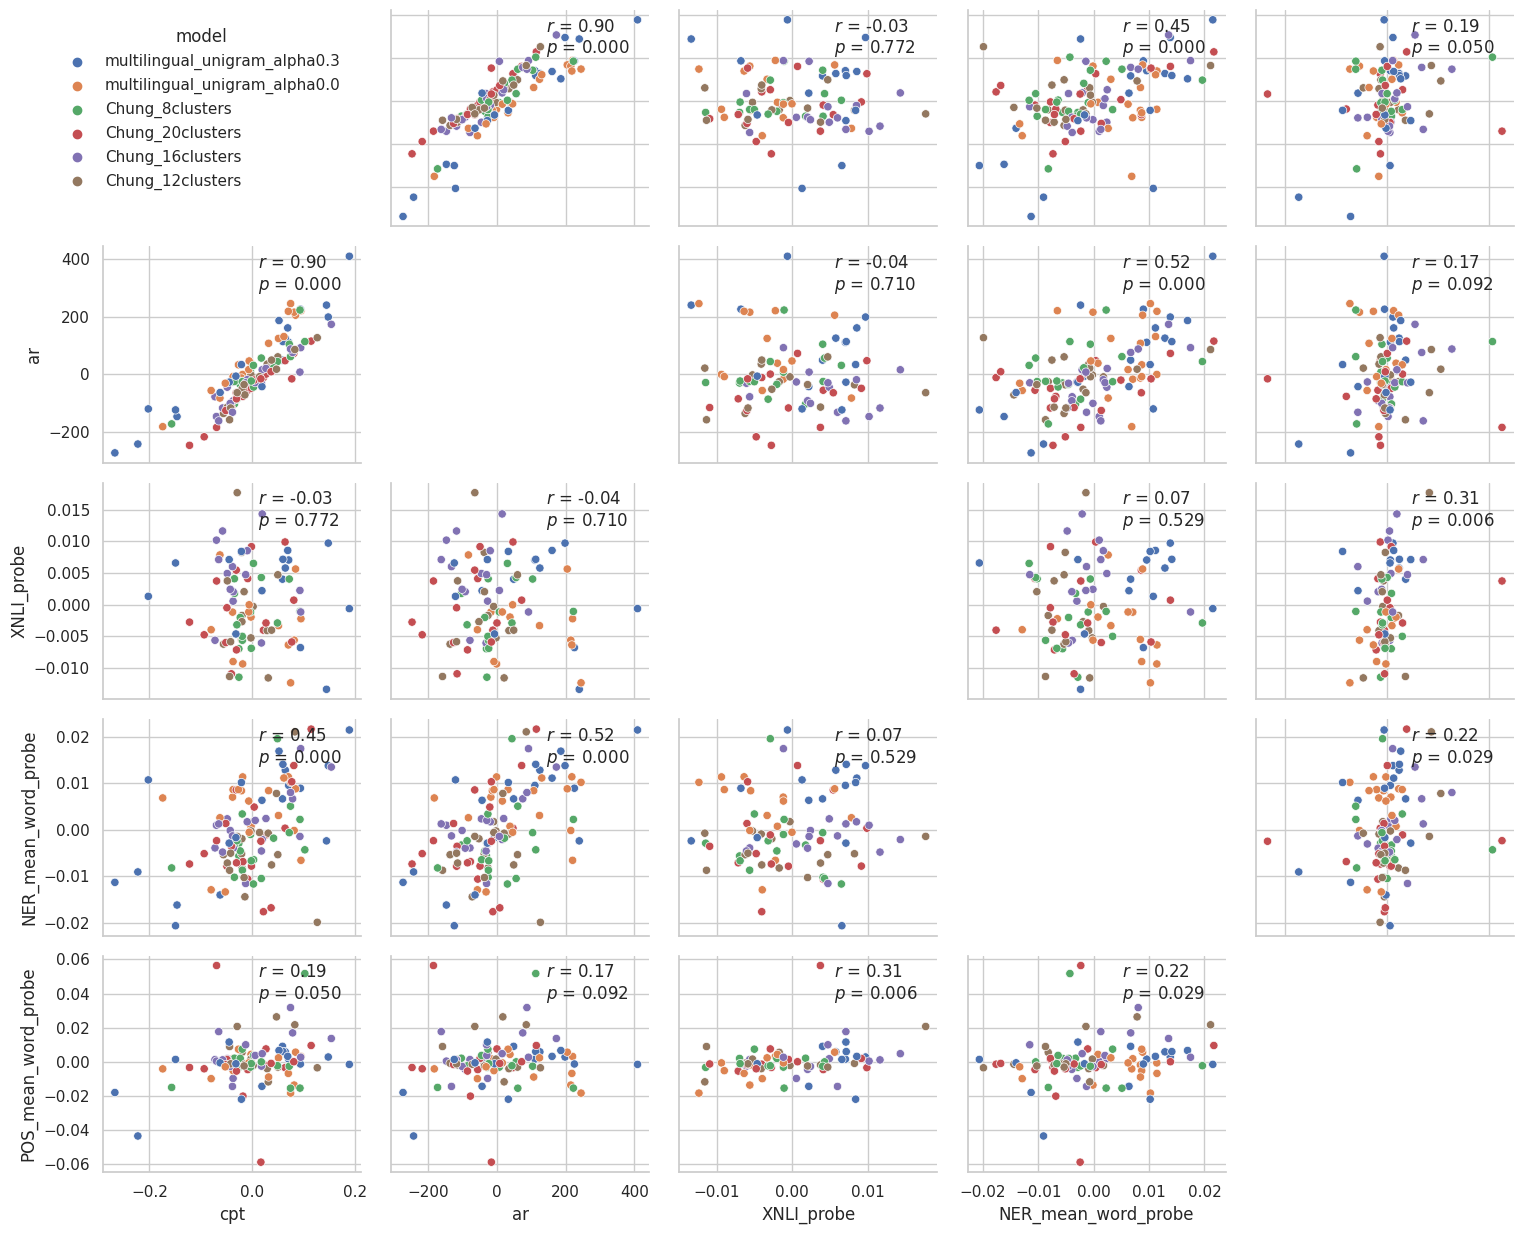
\includegraphics[width=\textwidth]{img/temp/probe_overall_inlanguage_scattermatrix.png}
    \caption{We visualize the in-language results from Figure \ref{fig:probe_overall_inlanguage} in a scatter matrix. We center the results for each language and then plot the differences from mean performance against the differences in our tokenizer metrics. We see significant spearman correlations for the NER and POS tasks, although for POS the correlation is low. For the NLI task, we do not observe any significant correlations.}
    \label{fig:probe_overall_inlanguage_scattermatrix}
\end{figure}


% \begin{figure}[H]
%     \centering
%     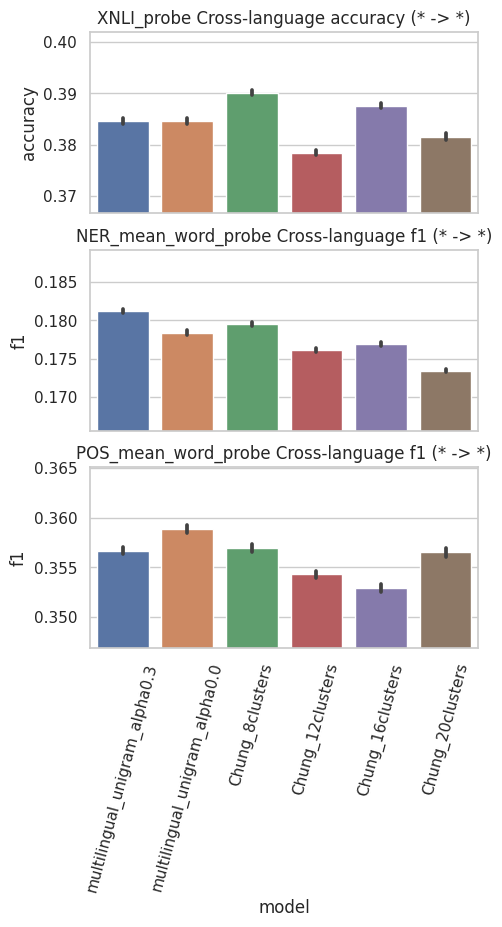
\includegraphics[width=\textwidth]{img/temp/probe_overall_crosslanguage.png}
%     \caption{probe overall crosslanguage}
%     \label{fig:probe_overall_crosslanguage}
% \end{figure}

\begin{figure}[H]
    \centering
    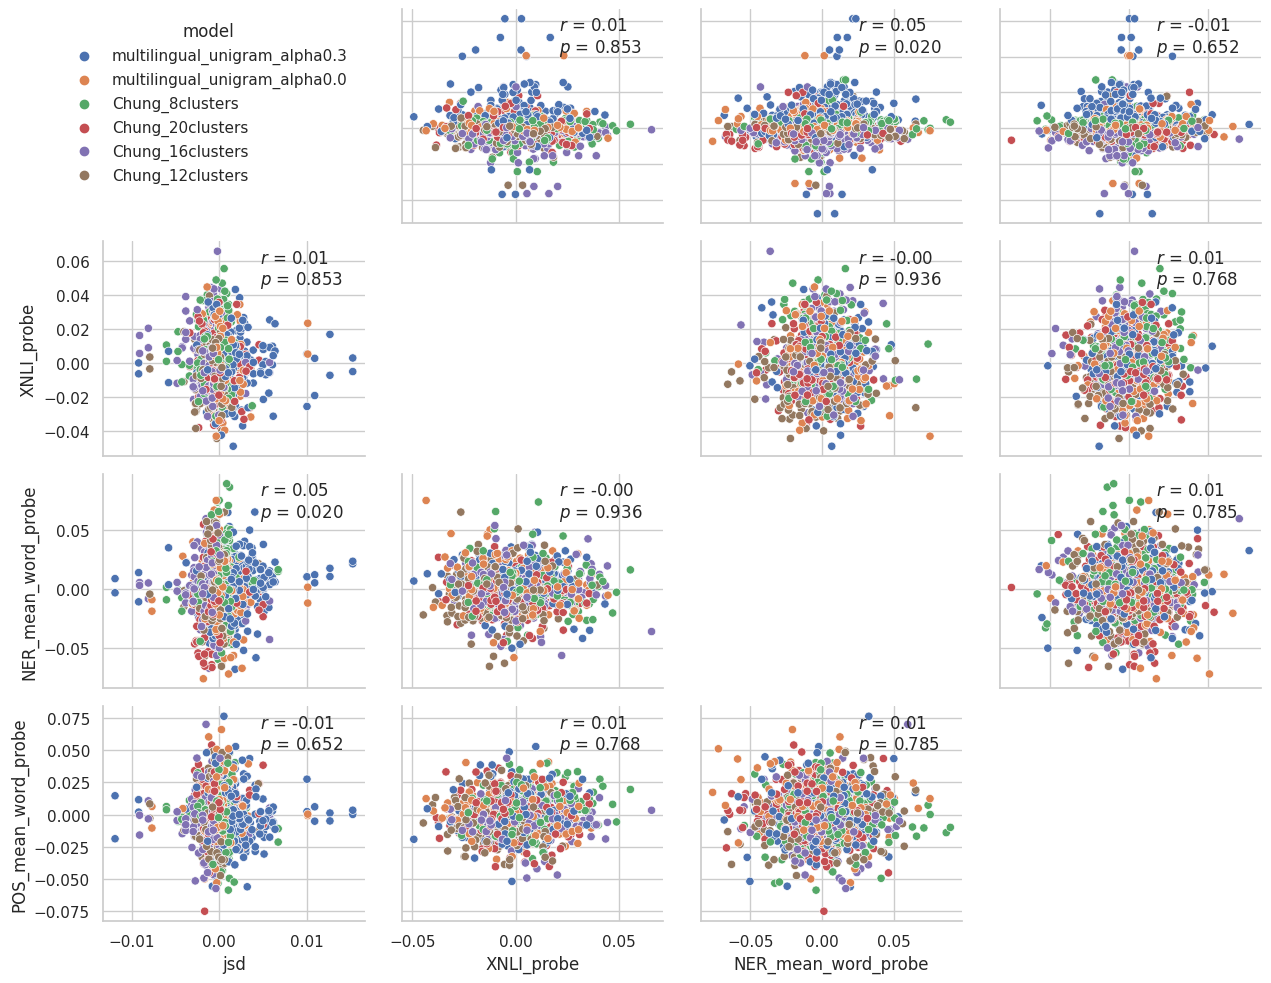
\includegraphics[width=\textwidth]{img/temp/probe_overall_crosslanguage_scattermatrix.png}
    \caption{We visualize the cross-language results from Figure \ref{fig:probe_overall_crosslanguage} in a scatter matrix. We center the results for each language and then plot the differences from mean performance against the differences in the vocabulary overlap metric (JSD). We see significant, very low negative correlation for the NER and POS tasks. This might suggest that the word-level tasks benefit only very slightly from an increase in overlap (decrease in JSD). For the NLI task, we do not observe any significant correlations.}
    \label{fig:probe_overall_crosslanguage_scattermatrix}
\end{figure}

% visualization idea:

% - visualization of tokenizer balance difference is too noisy to see the differences between methods
%     - smoothing num_lines_per_language vs cpt
%     - or fitting a line
%     - something that highlights if one balancing method is better than another

% \section{Preliminary experiments}
% \subsection{The importance of training data size}
% \subsection{Differences in tokenizer implementations}
% \section{Reproduction of baselines}
% \section{Document-level clustering method}
% \section{Extrinsic evaluation}


% - replication of the previous work
%     - Chung
%         - reproductions in Overlap-based Vocabulary Generation Improves Cross-lingual Transfer Among Related Languages

%     - Liang
%         - they use 900k vocab, they compare their model to XLM-R which is not fair!
%             - they discuss it in section 6.4
%         - reproductions: https://github.com/stefan-it/xlm-v-experiments
%             - For XQuAD they did not reproduce the improvements
%             - For MasakhaNER they reproduced the improvements
%             - TODO: could use bootstrapping to show whether the improvements are significant

% replications of Chung, Liang
% https://github.com/stefan-it/xlm-v-experiments

% - our beta experiments point to the randomness of the output - the smooth sweep across the beta values seems to produce quite noisy outpus


\chapter{Discussion}

- our comparison is limited to 20 langs and small models
    - it is not feasible for us to train Sentencepiece on more than 40M lines of text which limits the number of languages we can compare
    - this is a clear advantage of the Zheng method where they can train a separate tokenizer for each language - and thus overcome this liimtation.
- alpha0 assumes that we have enough data for each language
    - this might not be the case for some extremely-low-resource languages
    - it seems that we need atleast 100k lines to get good tokenizer for that language which is available for most languages
    - but this problem cannot be tackled by any method

% \include{intro}
% \chapter{Important first chapter}
\label{chap:refs}

First chapter usually builds the theoretical background necessary for readers to understand the rest of the thesis. You should summarize and reference a lot of existing literature and research.

You should use the standard \emph{citations}\todo{Use \textbackslash{}emph command like this, to highlight the first occurrence of an important word or term. Reader will notice it, and hopefully remember the importance.}.

\begin{description}
\item[Obtaining bibTeX citation] Go to Google Scholar\footnote{\url{https://scholar.google.com}}\todo{This footnote is an acceptable way to `cite' webpages or URLs. Documents without proper titles, authors and publishers generally do not form citations. For this reason, avoid citations of wikipedia pages.}, find the relevant literature, click the tiny double-quote button below the link, and copy the bibTeX entry.
\item[Saving the citation] Insert the bibTeX entry to the file \texttt{refs.bib}. On the first line of the entry you should see the short reference name --- from Scholar, it usually looks like \texttt{author2015title} --- you will use that to refer to the citation.
\item[Using the citation] Use the \verb|\cite| command to typeset the citation number correctly in the text; a long citation description will be automatically added to the bibliography at the end of the thesis. Always use a non-breakable space before the citing parenthesis to avoid unacceptable line breaks:
\begin{Verbatim}
Trees utilize gravity to invade ye
noble sires~\cite{newton1666apple}.
\end{Verbatim}
\item[Why should I bother with citations at all?] For two main reasons:
\begin{itemize}
\item You do not have to explain everything in the thesis; instead you send the reader to refer to details in some other literature. Use citations to simplify the detailed explanations.
\item If you describe something that already exists without using a citation, the reviewer may think that you \emph{claim} to have invented it. Expectably, they will demand academic correctness, and, from your perspective, being accused of plagiarism is not a good starting point for a successful defense. Use citations to identify the people who invented the ideas that you build upon.
\end{itemize}
\item[How many citations should I use?]
Cite any non-trivial building block or assumption that you use, if it is published in the literature. You do not have to cite trivia, such as the basic definitions taught in the introductory courses.

The rule of thumb is that you should read, understand and briefly review at least around 4 scientific papers. A thesis that contains less than 3 sound citations will spark doubt in reviewers.
\end{description}

There are several main commands for inserting citations, used as follows:
\begin{itemize}
\item \citet{knuth1979tex} described a great system for typesetting theses.
\item We are typesetting this thesis with \LaTeX, which is based on \TeX{} and METAFONT~\cite{knuth1979tex}.
\item \TeX{} was expanded to \LaTeX{} by \citet{lamport1994latex}, hence the name.
\item Revered are the authors of these systems!~\cite{knuth1979tex,lamport1994latex}
\end{itemize}

\section{Some extra assorted hints before you start writing English}

\paragraph{Word order}
Strictly adhere to the English word order rules. The sentences follow a fixed structure with a subject followed by a verb and an object (in this order). Exceptions to this rule must be handled specially, and usually separated by commas.

\paragraph{Sentence structure}
Do not write long sentences. One sentence should contain exactly one fact. Multiple facts should be grouped in a paragraph to communicate one coherent idea. Both the sentences and paragraphs should include various hints about their relation to the other ideas and paragraps. These are typically materialized as adverbs or short sentence parts that clarify the cause--outcome and target--method--result relationship of the sentences in a paragraph. Such `word glue' helps the readers to correctly draw the lines that hold their mental images of your thesis together, and ideally see the big picture of what you were trying to convey right from the first read.

Paragraphs are grouped in labeled sections for a sole purpose of making the navigation in the thesis easier. Do not use the headings as `names for paragraphs' --- the text should make perfect sense even if all headings are removed. If a section of your text contains one paragraph per heading, you might have wanted to write an explicit list instead.

Mind the rules for placing commas:
\begin{itemize}
\item Do not use the comma before subordinate clauses that begin with `that' (like this one). English does not use subordinate clauses as often as Slavic languages because the lack of a suitable word inflection method makes them hard to understand. In scientific English, try to avoid them as much as possible. Ask doubtfully whether each `which' and `when' is necessary --- most of these helper conjunctions can be removed by converting the clause to non-subordinate.

As an usual example, \xxx{\textit{`The sentence, which I wrote, seemed ugly.'}} is perfectly bad; slightly improved by \xxx{\textit{`The sentence that I wrote seemed ugly.'}}, which can be easily reduced to \textit{`The sentence I wrote seemed ugly.'}. A final version with added storytelling value could say \textit{`I wrote a sentence but it seemed ugly.'}
\item Use the \emph{Oxford comma} before `and' and `or' at the end of a longer, comma-separated list of items. Certainly use it to disambiguate any possible mixtures of conjunctions: \textit{`The car is available in red, red and green, and green versions.'} Remember that English `or' is typically understood more like `either this or that, but not both,' and the use of `and` is much more appropriate in cases such as possibility overviews and example listings (like in this sentence).
\item Consider placing extra commas around any parts of the sentence that break the usual word order, especially if they are longer than a single word.
\end{itemize}

\paragraph{Nouns}
Every noun needs a determiner (`a', `the', `my', `some', \dots); the exceptions to this rule, such as non-adjectivized names and indeterminate plural, are relatively scarce. Without a determiner, a noun can be easily mistaken for something completely different, such as an adjective or a verb.

Name all things with appropriate nouns to help both the reader and yourself, and do not hesitate to invent good names and labels for anything that you will refer to more than once. Proper naming will save you a lot of writing effort because you will not have to repeat descriptions such as \xxx{\textit{`the third output of the second benchmarked method of the improved set,'}} instead you may introduce a labeling that will allow you to say just something like \textit{`output M2\textsuperscript{+}-3'}. At the same time, this will reduce the risk that the reader will confuse the object with another one --- for illustration, the long version of the previous example might very easily confuse with the second output of the third method. The same also applies to methods descriptions, algorithms, programs, testing datasets, theorems, use-cases, challenges and other things. As an example, \xxx{\textit{`the algorithm that organizes the potatoes into appropriate buckets'}} shortens nicely as \textit{`the potato bucketer'} and may be labeled as a procedure \textsc{BucketPotatoes()}, and \xxx{\textit{`the issue where the robot crashes into a wall and takes significant time to return to the previous task'}} may be called just \textit{`the crash--recovery lag'}.

\paragraph{Verbs}
Although English can express a whopping 65 base verb tenses and their variants, scientific literature often suppresses this complexity and uses only several basic tenses where the meaning is clearly defined. Typically, you state facts in present simple (\textit{`Theorem 1 proves that Gadget B works as intended.'}), talk about previous work and experiments done in past simple (\textit{`We constructed Gadget B from Gizmo C, which was previously prepared by Tinkerer et al.'}), and identify achieved results in present perfect (\textit{`We have constructed Technology T.'}). Avoid using future tense, except for sections that explicitly describe future work --- as a typical mistake, if you state that the thesis \emph{will} describe something in later chapters, you imply that the description is not present there yet.

Do not write sentences in passive voice, unless you explicitly need to highlight that something has passively subjected itself to an action. Active voice is more preferable in the theses because it clearly highlights the actors and their contributions --- typically, \textit{`you did it'} instead of \textit{`it was done'} by a mysterious entity, which the reviewers rarely envision as yourself. Writing in active voice additionally benefits the explanation of complex processes: There, the word order forces you to identify the acting subject as the first word in the sentence, which further disambiguates how the individual process parts are triggered and ordered.

Try to avoid overusing gerunds (verbs that end with `-ing'). It is convenient to write shorter sentences by using gerunds as adjectives, but these are typically quite hard to understand because the readers may easily confuse the intended adjectives with verbs. If your sentence contains two gerunds close to each other, it may need a rewrite.

\paragraph{Scientific writing resources}
Consult the book by \citet{glasman2010science} for more useful details and recommended terminology for writing about the scientific research. Very pragmatically, the book by \citet{sparling1989english} describes many common mistakes that Czech and Slovak (and generally Slavic) writers make when writing English.

% \chapter{More complicated chapter}
\label{chap:math}

After the reader gained sufficient knowledge to understand your problem in \cref{chap:refs}, you can jump to your own advanced material and conclusions.

You will need definitions (see \cref{defn:x} below in \cref{sec:demo}), theorems (\cref{thm:y}), general mathematics, algorithms (\cref{alg:w}), and tables (\cref{tab:z})\todo{See documentation of package \texttt{booktabs} for hints on typesetting tables. As a main rule, \emph{never} draw a vertical line.}. \Cref{fig:f,fig:g} show how to make a nice figure. See \cref{fig:schema} for an example of TikZ-based diagram. Cross-referencing helps to keep the necessary parts of the narrative close --- use references to the previous chapter with theory wherever it seems that the reader could have forgotten the required context. Conversely, it is useful to add a few references to theoretical chapters that point to the sections which use the developed theory, giving the reader easy access to motivating application examples.

\section{Example with some mathematics}
\label{sec:demo}

\begin{defn}[Triplet]\label{defn:x}
Given stuff $X$, $Y$ and $Z$, we will write a \emph{triplet} of the stuff as $(X,Y,Z)$.
\end{defn}

\newcommand{\Col}{\textsc{Colour}}

\begin{thm}[Car coloring]\label{thm:y}
All cars have the same color. More specifically, for any set of cars $C$, we have
$$(\forall c_1, c_2 \in C)\:\Col(c_1) = \Col(c_2).$$
\end{thm}

\begin{proof}
Use induction on sets of cars $C$. The statement holds trivially for $|C|\leq1$. For larger $C$, select 2 overlapping subsets of $C$ smaller than $|C|$ (thus same-colored). Overlapping cars need to have the same color as the cars outside the overlap, thus also the whole $C$ is same-colored.\todo{This is plain wrong though.}
\end{proof}

\begin{table}
% uncomment the following line if you use the fitted top captions for tables
% (see the \floatsetup[table] comments in `macros.tex`.
%\floatbox{table}[\FBwidth]{
\centering\footnotesize\sf
\begin{tabular}{llrl}
\toprule
Column A & Column 2 & Numbers & More \\
\midrule
Asd & QWERTY & 123123 & -- \\
Asd qsd 1sd & \textcolor{red}{BAD} & 234234234 & This line should be helpful. \\
Asd & \textcolor{blue}{INTERESTING} & 123123123 & -- \\
Asd qsd 1sd & \textcolor{violet!50}{PLAIN WEIRD} & 234234234 & -- \\
Asd & QWERTY & 123123 & -- \\
\addlinespace % a nice non-intrusive separator of data groups (or final table sums)
Asd qsd 1sd & \textcolor{green!80!black}{GOOD} & 234234299 & -- \\
Asd & NUMBER & \textbf{123123} & -- \\
Asd qsd 1sd & \textcolor{orange}{DANGEROUS} & 234234234 & (no data) \\
\bottomrule
\end{tabular}
%}{  % uncomment if you use the \floatbox (as above), erase otherwise
\caption{An example table.  Table caption should clearly explain how to interpret the data in the table. Use some visual guide, such as boldface or color coding, to highlight the most important results (e.g., comparison winners).}
%}  % uncomment if you use the \floatbox
\label{tab:z}
\end{table}

\begin{figure}
\centering
\includegraphics[width=.6\linewidth]{img/ukazka-obr02.pdf}
\caption{A figure with a plot, not entirely related to anything. If you copy the figures from anywhere, always refer to the original author, ideally by citation (if possible). In particular, this picture --- and many others, also a lot of surrounding code --- was taken from the example bachelor thesis of MFF, originally created by Martin Mareš and others.}
\label{fig:g}
\end{figure}

\begin{figure}
\centering
\tikzstyle{box}=[rectangle,draw,rounded corners=0.5ex,fill=green!10]
\begin{tikzpicture}[thick,font=\sf\scriptsize]
\node[box,rotate=45] (a) {A test.};
\node[] (b) at (4,0) {Node with no border!};
\node[circle,draw,dashed,fill=yellow!20, text width=6em, align=center] (c) at (0,4) {Ugly yellow node.\\Is this the Sun?};
\node[box, right=1cm of c] (d) {Math: $X=\sqrt{\frac{y}{z}}$};
\draw[->](a) to (b);
\draw[->](a) to[bend left=30] node[midway,sloped,anchor=north] {flow flows} (c);
\draw[->>>,dotted](b) to[bend right=30] (d);
\draw[ultra thick](c) to (d);

\end{tikzpicture}
\caption{An example diagram typeset with TikZ. It is a good idea to write diagram captions in a way that guides the reader through the diagram. Explicitly name the object where the diagram viewing should ``start''. Preferably, briefly summarize the connection to the parts of the text and other diagrams or figures. (In this case, would the tenative yellow Sun be described closer in some section of the thesis? Or, would there be a figure to detail the dotted pattern of the line?)}
\label{fig:schema}
\end{figure}

\begin{algorithm}
\begin{algorithmic}
\Function{ExecuteWithHighProbability}{$A$}
	\State $r \gets$ a random number between $0$ and $1$
	\State $\varepsilon \gets 0.0000000000000000000000000000000000000042$
	\If{$r\geq\varepsilon$}
		\State execute $A$ \Comment{We discard the return value}
	\Else
		\State print: \texttt{Not today, sorry.}
	\EndIf
\EndFunction
\end{algorithmic}
\caption{Algorithm that executes an action with high probability. Do not care about formal semantics in the pseudocode --- semicolons, types, correct function call parameters and similar nonsense from `realistic' languages can be safely omitted. Instead make sure that the intuition behind (and perhaps some hints about its correctness or various corner cases) can be seen as easily as possible.}
\label{alg:w}
\end{algorithm}

\section{Extra typesetting hints}

Do not overuse text formatting for highlighting various important parts of your sentences. If an idea cannot be communicated without formatting, the sentence probably needs rewriting anyway. Imagine the thesis being read aloud as a podcast --- the storytellers are generally unable to speak in boldface font.

Most importantly, do \underline{not} overuse bold text, which is designed to literally \textbf{shine from the page} to be the first thing that catches the eye of the reader. More precisely, use bold text only for `navigation' elements that need to be seen and located first, such as headings, list item leads, and figure numbers.

Use underline only in dire necessity, such as in the previous paragraph where it was inevitable to ensure that the reader remembers to never typeset boldface text manually again.

Use \emph{emphasis} to highlight the first occurrences of important terms that the reader should notice. The feeling the emphasis produces is, roughly, ``Oh my --- what a nicely slanted word! Surely I expect it be important for the rest of the thesis!''

Finally, never draw a vertical line, not even in a table or around figures, ever. Vertical lines outside of the figures are ugly.

% \chapter{Results and discussion}

You should have a separate chapter for presenting your results (generated by the stuff described previously, in our case in \cref{chap:math}). Remember that your work needs to be validated rigorously, and no one will believe you if you just say that `it worked well for you'.

Instead, try some of the following:
\begin{itemize}
\item State a hypothesis and prove it statistically
\item Show plots with measurements that you did to prove your results (e.g. speedup). Use either \texttt{R} and \texttt{ggplot}, or Python with \texttt{matplotlib} to generate the plots.\footnote{Honestly, the plots from \texttt{ggplot} look \underline{much} better.} Save them as PDF to avoid printing pixels (as in \cref{fig:f}).
\item Compare with other similar software/theses/authors/results, if possible
\item Show example source code (e.g. for demonstrating how easily your results can be used)
\item Include a `toy problem' for demonstrating the basic functionality of your approach and detail all important properties and results on that
\item Include clear pictures of `inputs' and `outputs' of all your algorithms, if applicable
\end{itemize}

\begin{figure}
\centering
\includegraphics[width=.6\linewidth]{img/ukazka-obr01.pdf}
\caption{This caption is a friendly reminder to never insert figures ``in text,'' without a floating environment, unless explicitly needed for maintaining the text flow (e.g., the figure is small and developing with the text, like some of the centered equations, as in \cref{thm:y}). All figures \emph{must} be referenced by number from the text (so that the readers can find them when they read the text) and properly captioned (so that the readers can interpret the figure even if they look at it before reading the text --- reviewers love to do that).}
\label{fig:f}
\end{figure}

It is sometimes convenient (even recommended by some journals, including Cell) to name the results sub-sections so that they state what exactly has been achieved. Examples follow.

\section{SuperProgram is faster than OldAlgorithm}
\subsection{Scalability estimation}
\subsection{Precision of the results}
\section{Weird theorem is proven by induction}
\section{Amount of code reduced by CodeRedTool}
\subsection{Example}
\subsection{Performance on real codebases}
\section{\sloppy NeuroticHelper improves neural network learning}

\section{Graphics and figure quality}

No matter how great the text content of your thesis is, the pictures will always catch the attention first. This creates the very important first impression of the thesis contents and general quality. Crucially, that also decides whether the thesis is later read with joy, or carefully examined with suspicion.

Preparing your thesis in a way such that this first impression gets communicated smoothly and precisely helps both the reviewer and you: the reviewer will not have a hard time understanding what exactly you wanted to convey, and you will get a better grade.

Making the graphics `work for you' involves doing some extra work that is often unexpected. At the same time, you will need to fit into graphics quality constraints and guidelines that are rarely understood before you actually see a bad example. As a rule of thumb, you should allocate at least the same amount of time and effort for making the figures look good as you would for writing, editing and correcting the same page area of paragraph text.

\subsection{Visualize all important ideas}
The set of figures in your thesis should be comprehensive and complete. For all important ideas, constructions, complicated setups and results there should be a visualization that the reader can refer to in case the text does not paint the `mental image' sufficiently well. At the bare minimum, you should have at least 3 figures (roughly corresponding to the 3 chapters) that clearly and unambiguously show:
\begin{enumerate}
\item the context of the problem you are solving, optionally with e.g.~question marks and exclamation marks placed to highlight the problems and research questions
\item the overall architecture of your solution (usually as a diagram with arrows, such as in \cref{fig:schema}, ideally with tiny toy examples of the inputs and outputs of each box),
\item the advancement or the distinctive property of your solution, usually in a benchmark plot, or as a clear demonstration and comparison of your results.
\end{enumerate}

\subsection{Make the figures comprehensible}
The figures should be easily comprehensible. Surprisingly, that requires you to follow some common ``standards'' in figure design and processing. People are often used to a certain form of the visualizations, and (unless you have a very good reason) deviating from the standard is going to make the comprehension much more complicated. The common standards include the following:
\begin{itemize}
  \item caption everything correctly, place the caption at an expectable position
  \item systematically label the plots with `main' titles (usually in boldface, above the plot), plot axes, axis units and ticks, and legends
  \item lay out the diagrams systematically, ideally follow a structure of a bottom-up tree, a left-to-right pipeline, a top-down layered architecture, or a center-to-borders mindmap
  \item {use colors that convey the required information correctly \par\footnotesize Although many people carry some intuition for color use, achieving a really correct utilization of colors is often very hard without previous experience in color science and typesetting. Always remember that everyone perceives color hues differently, therefore the best distinction between the colors is done by varying lightness of the graphics elements (i.e., separating the data by dark vs.~light) rather than by using hues (i.e., forcing people to guess which one of salmon and olive colors means ``better''). Almost 10\% of the population have their vision impaired by some form of color vision deficiency, most frequently by deuteranomaly that prevents interpretation of even the most `obvious' hue differences, such as green vs.~red. Finally, printed colors look surprisingly different from the on-screen colors. You can prevent much of these problems by using standardized palettes and well-tested color gradients, such as the ones from ColorBrewer\footnote{\url{https://colorbrewer2.org}} and ViridisLite\footnote{\url{https://sjmgarnier.github.io/viridisLite/}}. Check if your pictures still look good if converted to greyscale, and use a color deficiency simulator to check how the colors are perceived with deuteranomaly.}
\end{itemize}

Avoid large areas of over-saturated and dark colors:
\begin{itemize}
  \item under no circumstances use dark backgrounds for any graphical elements, such as diagram boxes and tables --- use very light, slightly desaturated colors instead
  \item avoid using figures that contain lots of dark color (as a common example, heatmaps rendered with the `magma' color palette often look like huge black slabs that are visible even through the paper sheet, thus making a dark smudge on the neighboring page)
  \item increase the brightness of any photos to match the average brightness of the text around the figure
\end{itemize}

Remember to test your figures on other people --- usually, just asking `What do you think the figure should show?' can help you debug many mistakes in your graphics. If they think that the figure says something different than what you planned, then most likely it is your figure what is wrong, not the understanding of others.

Finally, there are many magnificent resources that help you arrange your graphics correctly. The two books by Tufte~\cite{tufte1990envisioning,tufte1983visual} are arguably classics in the area. Additionally, you may find many interesting resources to help you with technical aspects of plotting, such as the \texttt{ggplot}-style `Fundamentals' book by~\citet{wilke2019fundamentals}, and a wonderful manual for the TikZ/PGF graphics system by~\citet{tantau2015tikz} that will help you draw high-quality diagrams (like the one in~\cref{fig:schema}).

\section{What is a discussion?}
After you present the results and show that your contributions work, it is important to \emph{interpret} them, showing what they mean in the wider context of the thesis topic, for the researchers who work in the area, and for the more general public, such as for the users.

Separate discussion sections are therefore common in life sciences where some ambiguity in result interpretation is common, and the carefully developed intuition about the wider context is sometimes the only thing that the authors have. Exact sciences and mathematicians do not need to use the discussion sections as often. Despite of that, it is nice to position your output into the previously existing environment, answering:
\begin{itemize}
\item What is the potential application of the result?
\item Does the result solve a problem that other people encountered?
\item Did the results point to any new (surprising) facts?
\item How (and why) is the approach you chose different from what the others have done previously?
\item Why is the result important for your future work (or work of anyone other)?
\item Can the results be used to replace (and improve) anything that is used currently?
\end{itemize}

If you do not know the answers, you may want to ask the supervisor. Also, do not worry if the discussion section is half-empty or thoroughly pointless; you may remove it completely without much consequence. It is just a bachelor thesis, not a world-saving avenger thesis.

% 
\chapter{Conclusion}
\label{chap:conclusion}

% In the conclusion, you should summarize what was achieved by the thesis. In a few paragraphs, try to answer the following:
% \begin{itemize}
% \item Was the problem stated in the introduction solved? (Ideally include a list of successfully achieved goals.)
% \item What is the quality of the result? Is the problem solved for good and the mankind does not need to ever think about it again, or just partially improved upon? (Is the incompleteness caused by overwhelming problem complexity that would be out of thesis scope\todo{This is quite common.}, or any theoretical reasons, such as computational hardness?)
% \item Does the result have any practical applications that improve upon something realistic?
% \item Is there any good future development or research direction that could further improve the results of this thesis? (This is often summarized in a separate subsection called `Future work'.)
% \end{itemize}

% Introduction

% In this thesis, we ask what makes a good tokenization method for multilingual models, how to measure it and what factors influence it \tomasz{isn't it also a research question?}. Moreover, our focus is achieving better tokenization for all languages, especially the ones that have been shown to be underrepresented in the previous multilingual models \cite{rust_how_2021}. We fill a methodological gap by proposing a robust set of metrics for measuring the quality of tokenization methods in the multilingual setting. Our metrics measure whether tokenizers effectively represent meaningful language-specific tokens in the vocabulary (\textit{vocabulary allocation}) and whether the units they learn are shared across languages (\textit{vocabulary overlap}). The questions we address are: \textbf{Q1:} How do subword tokenizers differ in overlap and allocation of learned vocabularies? And \textbf{Q2:} Which properties of multilingual tokenizers affect the language model representation quality?

% After we establish our metrics, we address the underresearched question of \textbf{Q3:} What is the reason that the standard tokenizer training method does not work well in the multilingual setting? To this end, we examine the effect of the training data size, character coverage, and most importantly, the data imbalance between high-resource and low-resource languages present in the tokenizer training data. We find that the data imbalance has a significant effect on the resulting tokenizer and by balancing the training data, we can achieve better tokenization for all languages.

% With our new analytical tools for the standard tokenization methods and their properties, we turn to the three existing works by \citet{chung_improving_2020,zheng_allocating_2021,liang_xlm-v_2023} which we collectively address to as "balancing methods" proposed for improving tokenization for all training languages. We find that the three works report empirical improvements of their methods but compare themselves to highly unbalanced baselines. We therefore ask \textbf{Q4:} What is the effect of using the vocabulary balancing methods on the representation of low-resource languages? And
% \textbf{Q5:} How do the vocabulary balancing methods compare to the standard method of training the tokenizer on balanced and unbalanced joint corpus?

% Through in-depth analysis, we find that the three methods we reproduce \cite{chung_improving_2020,zheng_allocating_2021,liang_xlm-v_2023} improve tokenization by balancing the \textit{vocabulary allocation} between the languages. We further show, that in our setting, similar results can be achieved by a simpler method of uniform sampling of languages during the tokenizer training. 

% Findings of Experimental chapter 1

% \textbf{Q1:} How do subword tokenizers differ in overlap and allocation of learned vocabularies?
% \textbf{Q2:} Which properties of multilingual tokenizers affect the language model representation quality?

% We find that the choice of the tokenization method largely influences the vocabulary allocation and overlap metrics (\textbf{Q1}). We see that Huggingface BPE better allocates the vocabulary overall and has a lower overlap between languages. On the other hand, the Huggingface Unigram tokenizer segments the text into shorter tokens and the average vocabulary overlap between all languages is much higher.

% We find that the differences between tokenizers are reflected in the representation quality (\textbf{Q2}). High vocabulary allocation metrics are correlated with better probe performance, especially on the word-level tasks. Moreover, the cross-lingual performance is correlated with higher vocabulary allocation and lower overlap.

% Findings of Experimental chapter 2

% In this chapter, we have investigated \textbf{Q3:} What is the reason that the standard tokenizer training method does not work well in the multilingual setting? To this end, we explore how different design choices affect the quality of the tokenizers. 

% We find that the implementation of the Unigram algorithm in the Huggingface library is subpar and that the Sentencepiece implementation yields better results.

% We observe that we need around 100k-1M lines per language to train a good, multilingual tokenizer. 

% The alphabet size affects the number of UNK tokens but does not have a significant influence on the rest of the metrics if we stay in the range of 1000-5000 alphabet size. 

% Most importantly, we observe that tokenizer training data imbalance influences the per-language metrics heavily and that it lowers the tokenization quality for the low-resource languages more than it improves it for the high-resource.

% Findings of Experimental chapter 3


% \textbf{Q4:} What is the effect of using the reproduced methods on the representation of low-resource languages? And
% \textbf{Q5:} How do the reproduced methods compare to the standard method of training the tokenizer on balanced and unbalanced joint corpus?

% We find that the balancing methods of \citet{chung_improving_2020,zheng_allocating_2021,liang_xlm-v_2023} improve the representation of low-resource languages by increasing the \textit{vocabulary allocation} for these languages at the cost of lowering the \textit{vocabulary allocation} for the high-resource ones. 

% We also find that the Unigram tokenizer trained with a balanced dataset ($\alpha=0.0$) achieves a similar effect as the replicated methods. 

% We find a striking similarity between the Unigram tokenizer trained on a balanced dataset and the Zheng method. We find that by maximizing the ALP across languages, Zheng method achieves a similar effect to running an Unigram tokenizer training on a balanced dataset.

% We find that the clustering methods with a high number of clusters behave similarly to the Unigram tokenizer trained on a balanced dataset. We assume that the reason is that the clustering methods with a high $k$ are similar to the Zheng method in that they train separate tokenizers for the majority of languages and only a few languages are grouped together.

% On the other hand, we find that the clustering methods with lower number of clusters are susceptible to a decrease in performance when high-resource and low-resource languages are assigned to the same cluster.

% By running the extrinsic evaluation, we validate the observations we made using the intrinsic evaluation. We find that the balancing methods improve the word-level tasks for low-resource languages while having no impact on the sentence-level task. 

% Interestingly, we find that the balancing has a net-positive effect for cross-lingual transfer across all languages.

% Our findings suggest that in our scaled-down setting of 20 languages and 120k vocabulary size, the simpler method of training a standard Unigram tokenizer on a joint, balanced corpus is sufficient to create a good multilingual vocabulary that represents all languages well.


% \textbf{Q1:} How do subword tokenizers differ in overlap and allocation of learned vocabularies?
% \textbf{Q2:} Which properties of multilingual tokenizers affect the language model representation quality?
% \textbf{Q3:} What is the reason that the standard tokenizer training method does not work well in the multilingual setting? 
% \textbf{Q4:} What is the effect of using the reproduced methods on the representation of low-resource languages? And
% \textbf{Q5:} How do the reproduced methods compare to the standard method of training the tokenizer on balanced and unbalanced joint corpus?

In this thesis, our main focus was to explore the characteristics of tokenization methods for multilingual models and investigate their impact on language model representation quality. 

To this end, we proposed a set of metrics for measuring the vocabulary allocation and overlap of tokenizer vocabularies. We compared our metrics to existing ones and we proposed a set of experiments to validate the usefulness of our metrics and investigate the properties of tokenization methods. 

We found that our metrics are useful for assessing the differences between tokenization methods and that vocabulary allocation and overlap are good predictors of language model performance for word-level tasks. Especially when considering word-level downstream tasks, the learned contextualized representations are better when the tokenizer segments the text into longer tokens (high characters per token), when the tokenizer allocates tokens more uniformly (high average rank), and when there is less overlap between the languages (high Jensen-Shannon divergence).
% ADD? Especially when considering word-level downstream tasks, the learned contextualized representations are better when the tokenizer segments the text into longer tokens (high characters per token), when the tokenizer allocates tokens more uniformly (high average rank), and when there is less overlap between the languages (high Jensen-Shannon divergence).

% We found that the choice between Unigram and BPE algorithms implemented in the Huggingface library significantly influences vocabulary allocation and overlap metrics. We also discovered that high vocabulary allocation correlated with improved representation quality, particularly on word-level tasks and cross-lingual performance.

With our established methodological framework, we then investigated the reasons for the subpar performance of standard tokenization methods in the multilingual setting. We demonstrated that to train a satisfactory tokenizer, we need around 100k to 1M lines of text per language. We also showed that the alphabet size does not largely affect our proposed metrics and that the default setting of covering 99.95\% of Unicode characters leads to a well performing tokenizer. 

We found that the main factors impacting the tokenization quality are the choice of implementation and data imbalance. We found that the Huggingface library yields subpar Unigram tokenizers and using the original Sentencepiece library mitigates a large gap in vocabulary allocation metrics we observed. More importantly, our research highlighted the strong impact of the data imbalance between high-resource and low-resource languages on the resulting tokenizer. 

Our experiments indicate, that the standard tokenizer training method is susceptible to training data imbalance which leads to a decrease in tokenization quality for the low-resource languages. Sampling data uniformly from each language during the tokenizer training mitigates this effect and leads to a better tokenization for the underresourced languages at a smaller cost on the high-resource.

After investigating the standard tokenization scheme, we turned our attention to three existing works by \citet{chung_improving_2020,zheng_allocating_2021,liang_xlm-v_2023} proposed for improving tokenization for low-resource languages. We identified that these vocabulary balancing methods use a highly unbalanced baseline to report their empirical improvements. We therefore investigated, how exactly these methods improve the tokenization quality for low-resource languages and how they compare to the standard method of training the tokenizer on a balanced and unbalanced joint corpus.

We found a surprising correspondence between the balancing methods and the Unigram tokenizer trained on a uniformly sampled dataset. We found that the balancing methods improve the tokenization quality for low-resource languages by increasing the vocabulary allocation for these languages at the cost of lowering the vocabulary allocation for the high-resource ones, similar to the standard method trained on uniformly sampled languages. Moreover, we found that the methods based on clustering are susceptible to a decrease in performance when high-resource and low-resource languages are assigned to the same cluster.

Our findings show that for all methods, the improvements on low-resource representation translate to improvement in word-level tasks in both in-language setting as well as cross-lingual transfer. 

Overall, our findings contribute to understanding tokenization methods for multilingual models. We propose a methodology for assessing the differences between tokenizers, emphasize the importance of selecting appropriate implementation, training parameters and data balance, and we show that with proper care, the simpler tokenization method of training a tokenizer on joint, multilingual corpus can achieve similar results to the balancing methods in our experimental setting.

\section{Limitations and future work}
% - our comparison is limited to 20 langs and small models
%     - it is not feasible for us to train Sentencepiece on more than 40M lines of text which limits the number of languages we can compare
%     - this is a clear advantage of the Zheng method where they can train a separate tokenizer for each language - and thus overcome this liimtation.
%     - we still believe that our methodology is a contribution in itself and following it we could compare the methods on a larger scale, if we had access to more computational resources
%         - for example we could pose the question after how many languages does the Zheng method become better than Sentencepiece Unigram. Then we could investigate which parameters could influence this possible detriment in performance (number of init sentencepieces, pruning steps etc.)
% - we also focus heavily on Sentencepiece Unigram as it is the most popular method. From our experiments it seems that Huggingface BPE is a good alternative to Sentencepiece Unigram and it would be interesting to compare it to the other methods
% - limitation - we didnt investigate BPE more in depth

Lastly, we acknowledge that due to computational limitations, we were not able to compare tokenizers on a larger scale. The language models were scaled down, the training data subsampled, vocabulary size reduced, and the number of languages limited to 20. We believe that our methodology is a contribution in itself and following it leads to a better understanding of the reasons for the differences between tokenizers. On the other hand, we are aware that the findings of our experiments are limited to the experimental setting we used. 

For future work, we would like to explore our research questions on a larger scale. Moreover, it would be interesting to investigate deeper the Huggingface BPE tokenizer as we found it to have the best overall performance in our experiments.

% For example, we could pose the question after how many languages does the Zheng method become better than Sentencepiece Unigram. Then we could investigate which parameters could influence this possible detriment in performance (number of init sentencepieces, pruning steps etc.).


\include{bibliography}

\appendix
% \include{howto}

% if your attachments are complicated, describe them in a separate appendix
%\include{attachments}

\openright
\end{document}
